\documentclass[12pt,a4paper]{article}
\usepackage{lastpage}
\usepackage{fancyhdr}
\pagestyle{fancy}
\usepackage{ dsfont }
\usepackage{hyperref}
\usepackage{graphicx}
\usepackage{subcaption}
\usepackage{float}
\usepackage{multirow}
\usepackage{array}
\usepackage{geometry}
\geometry{
    left=2cm,
    right=2cm,
    top=2cm,
    bottom=2cm
}
\usepackage{setspace}
\onehalfspacing
\usepackage{listings}
\bibliographystyle{IEEEtran}
\usepackage{xcolor}
\lstset{
    language=C++,                  % Set your language (you can change it as needed)
    basicstyle=\ttfamily\small,     % The basic style of your code
    keywordstyle=\color{blue},      % Keyword style
    stringstyle=\color{red},        % String literal style
    commentstyle=\color{gray},     % Comment style
    morecomment=[l][\color{magenta}]{\#},  % Directive style (like #include)
    numbers=left,                   % Line numbers on left
    numberstyle=\tiny\color{gray},  % Line number style
    stepnumber=1,                   % Line number step
    numbersep=5pt,                  % How far the line numbers are from the code
    backgroundcolor=\color{white},  % Background color for code block
    tabsize=2,                      % Tab size
    showspaces=false,               % Show spaces adding particular underscores
    showstringspaces=false,         % Underline spaces within strings only
    showtabs=false,                 % Show tabs within strings adding particular underscores
    frame=single,                   % Adds a frame around the code
    captionpos=b,                   % Sets the caption-position to bottom
    breaklines=true,                % Sets automatic line breaking
    breakatwhitespace=false,        % Sets if automatic breaks should only happen at whitespace
    escapeinside={\%*}{*)},         % If you want to add LaTeX within your code
}

\rhead{2131917, Page~\thepage~of~\pageref{LastPage}}
\newcolumntype{M}[1]{>{\centering\arraybackslash}p{#1}}
\begin{document}
\begin{center}
    \section*{HumanMade: A Platform for Verified Human Creations}
    \textbf{Author:} Luca Sarif-Kattan\\
    \textbf{Supervisor:} Ligang He\\
    \textbf{Year of study:} 2024\\
    \textbf{Keywords:} AI, Generative AI, Human, Creations, Blockchain, Web App, Node.js, Neural Network
\end{center}

\newpage

\noindent \textbf{Abstract:} With the dawn of generative AI, the landscape of human creativity and ingenuity is increasingly encroached upon. It is clear to most experts that this trend will continue in some fashion \cite{aiimpacts}, and there is a high chance that the entire creative space will be heavily dominated by AI in the near future. Due to the anthropocentric worldviews many of us hold \cite{anthropocentric} and to retain the pride of the human identity, having a platform which supports and incentivises human creation seems like it will be an in-demand product, and a beneficial necessity. HumanMade seeks to do this whilst avoiding the flawed approach of directly detecting AI-generated content, by:
\begin{itemize}
    \item Giving humans an easy way to document and upload their Creations
    \item Ensuring Creations are tamper-proof and traceable to the original creator
    \item Enabling and empowering the community of users to decide what they think is human-made and deserves their attention
\end{itemize}

\vspace{10pt}
\noindent \textbf{Acknowledgements:} I would like to thank myself for my amazing ideas, skilled programming and genius-level problem solving. I would like to thank Ligang He for a frictionless and enjoyable supervisor experience.

\newpage
\tableofcontents
\newpage

\section{Motivators}
\subsection{The Generative AI Explosion}
We are currently (March of 2024) in the midst of a generative AI (GAI) arms race. ChatGPT managed to reach 100 million users in 2 months \cite{gptstatistics}. Incredible advancements are being made weekly. More broadly, experts are predicting High-Level Machine Intelligence by 2059 \cite{aiimpacts}, and this is an exponentially decaying timeline, down 8 years from the previous time the survey was given. Here are some of the main reasons for this current AI explosion:
\begin{itemize}
    \item \textbf{Advancements in hardware.} The architectures which a lot of these models are based off of were discovered a while ago, (for example, the seminal Attention Is All You Need paper which introduced the highly popular transformer architecture was released in 2017 \cite{attention}), but recently we have witnessed huge improvements in the AI accelerated hardware needed to scale these models. Examples include Google's development of the TPU \cite{tpu}, and Nvidia's development of the Ampere architecture line of GPUs. GAI models require large-scale compute for the training phase. 
    \begin{figure}[H]
        \centering
        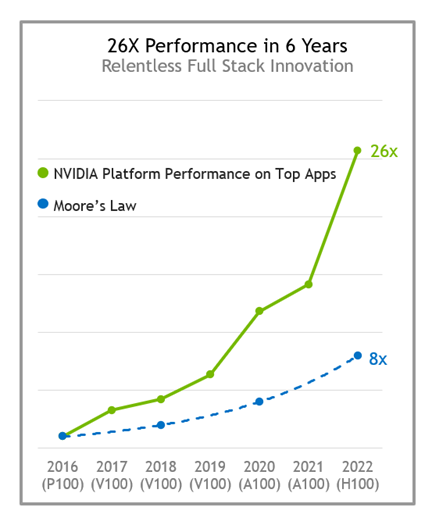
\includegraphics[scale=0.6]{nvidiaGraph.png}
        \cite{nvidia}
        \caption{A comparison of Nvidia hardware progress compared to Moore's law. The A100 GPU was used to train OpenAI's GPT-4. \cite{gpt4}}
    \end{figure}

    \item \textbf{Lack of regulations and restrictions.} There are currently no restrictions on the development of such technologies in the US, and the EU has introduced limited restrictions in the new AI act \cite{aiact}. There are obvious geopolitical incentives to allow the acceleration of GAI technologies, and open letters calling to pause giant AI experiments have failed to bring action \cite{fol}.
    \item \textbf{Profit incentives.} Such technologies are applicable across a huge spectrum of high-level tasks. There was 14 billion dollars in funding in 2023 towards GAI technologies \cite{genfunding}.
\end{itemize}
\subsection{A Look at the SOTA}
 A big part of the motivation for such a project comes from the unbelievable progress and ability of current GAI models, and how we might attempt to improve their detection. Therefore, in this section we take a brief look into the current state-of-the-art in GAI. At the moment there are two dominant model types:
\begin{itemize}
    \item Transformer models, used for text generation
    \item Diffusion models, used for image and video generation
\end{itemize}
Transformers were initially designed for NLP tasks, but have proven to be incredibly versatile and scalable \cite{scaling}. Performance has increased linearly with model size, even as model sizes have increased to trillions of parameters. 
\begin{figure}[H]
    \centering
    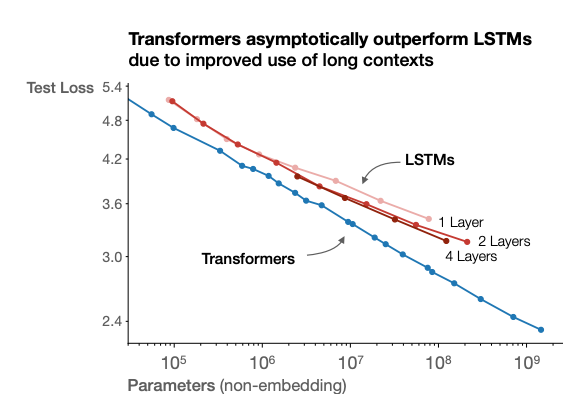
\includegraphics[scale=1]{linearScaling.png}
    \caption{Test loss (performance) against size (parameter count) of a model}
\end{figure}
\noindent SOTA for Transformers is currently Claude Opus, recently released by Anthropic. A few stats include Opus achieving 86.8\% on the MMLU (Undergraduate level multiple choice test) and 84.9\% on the HumanEval code benchmark \cite{opus}.
\\\\
Diffusion models gradually transform noise into a coherent image, based on learned data distributions. The SOTA is inherently more subjective in this area, but Midjourney version 5 is widely regarded as a front-runner in image generation. Midjourney can generate extremely detailed images from highly specific prompts.
\begin{figure}[H]
    \centering
    
\includegraphics[scale=0.4]{turtle.png}
    \caption{Generated using Midjourney with the prompt: `A scholarly turtle wearing glasses and a graduation cap, sitting in front of a stack of books. He has a wise and contemplative expression, as if lost in philosophical thought'}
\end{figure}
\noindent SOTA in video generation is clearly Sora, a recently released model from OpenAI which took the industry by surprise. Essentially working by diffusion but on multiple frames, Sora can also take in highly specific prompts and output detailed and realistic videos. 
\begin{figure}[H]
    \centering
    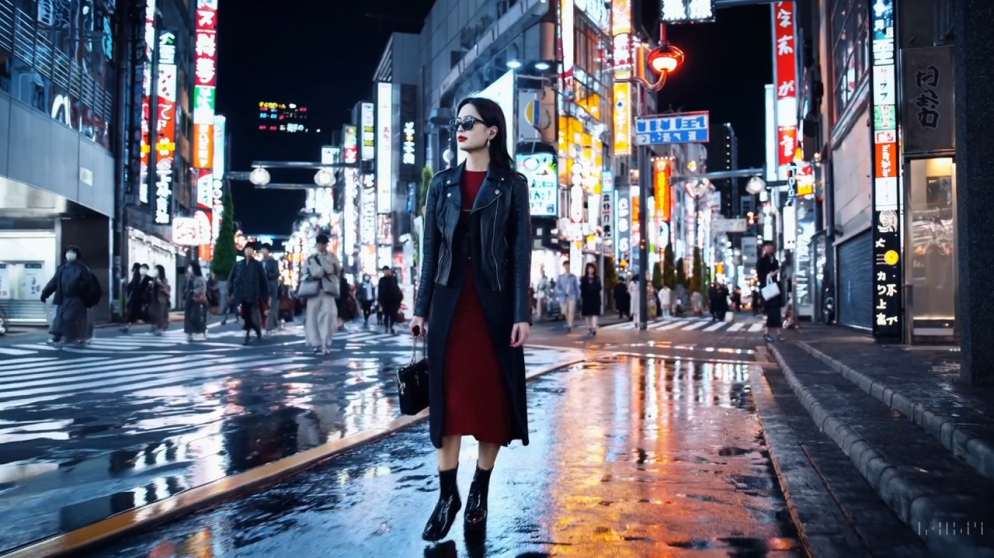
\includegraphics[scale=0.4]{sora.jpg}
    \caption{A frame from a Sora video, generated with the prompt: `A stylish woman walks down a Tokyo street filled with warm glowing neon and animated city signage. She wears a black leather jacket, a long red dress, and black boots, and carries a black purse. She wears sunglasses and red lipstick. She walks confidently and casually. The street is damp and reflective, creating a mirror effect of the colorful lights. Many pedestrians walk about.'}
\end{figure}
\subsection{The Need to Preserve Human Creativity}
The implication is that soon, we will be inundated with synthetic media and art. Whilst it is important to preserve human creations for philosophical reasons like maintaining the human identity, creative spirit and pride, there are two clearer motivators for building HumanMade:
\begin{enumerate}
    \item There will be free-market demand for authentic, human made creativity
    \item There is demand for general GAI detection and tracking
\end{enumerate}
Expanding on the first - recent research (perhaps unsurprisingly) shows a clear bias in humans towards human made art \cite{anthropocentric}. In this study, participants in different groups were presented with the same piece of art, but labelled as either human made or AI made. These labels directly affected a participants' preference to buy the art, via biased perceptions of the creativity and awe they felt towards it.
\begin{figure}[H]
    \centering
    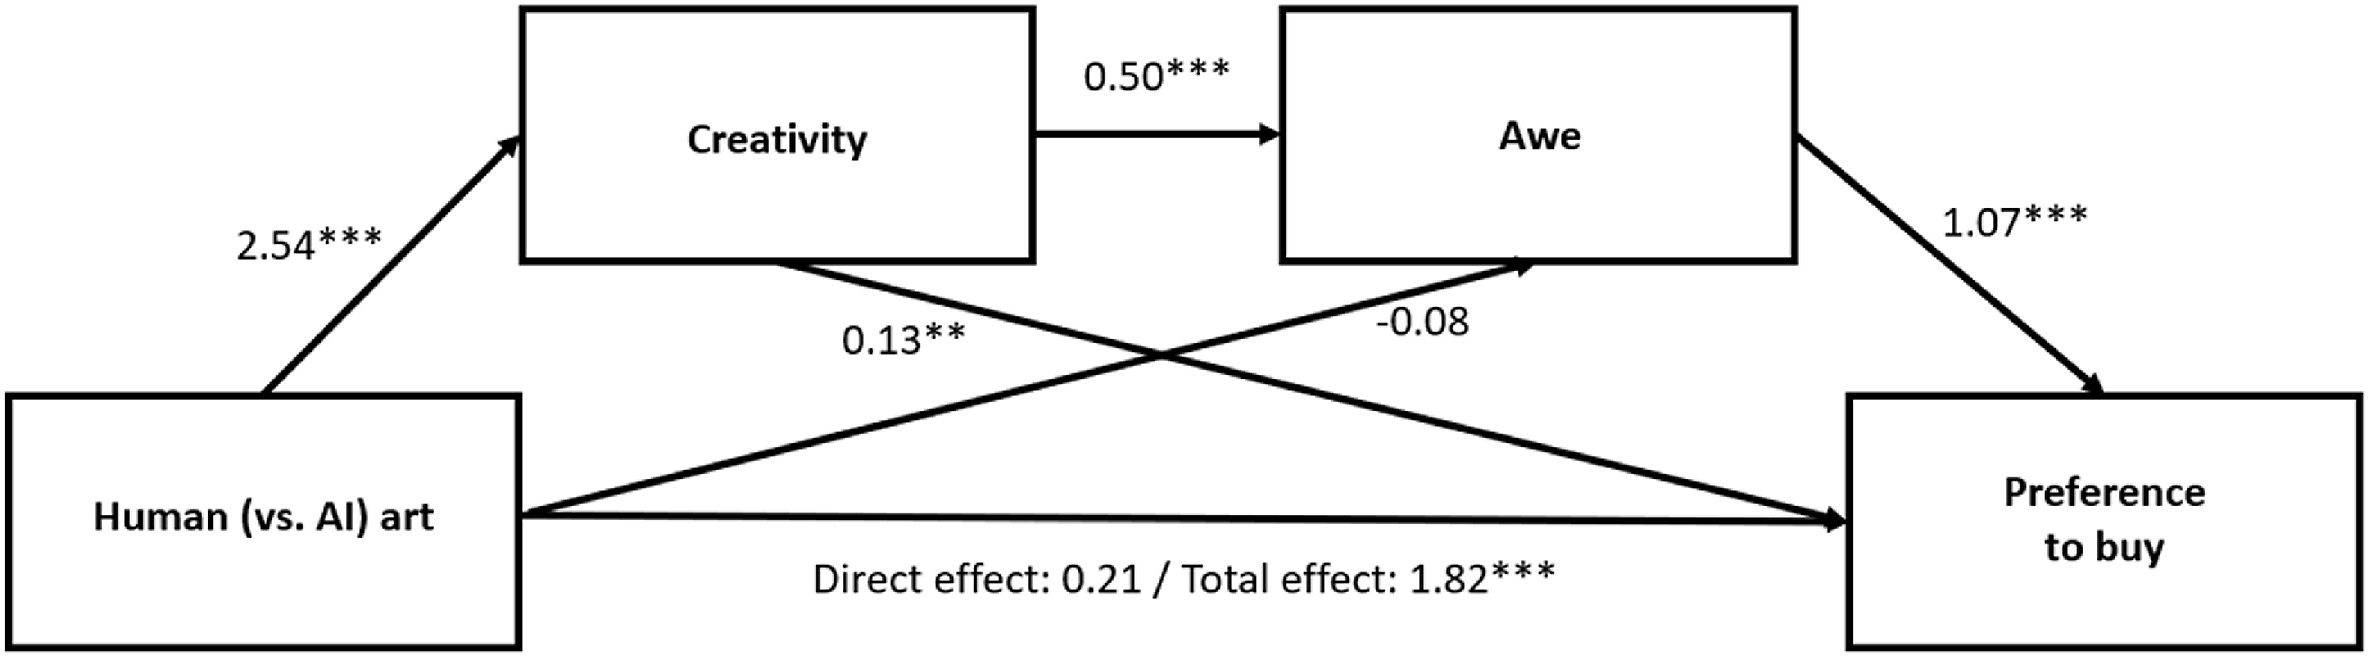
\includegraphics[scale=1]{biasDiagram.jpg}
    \caption{Indirect effect of human (vs. AI) art on preference to buy via perceived creativity and experienced awe.}
\end{figure}

\noindent Expanding on the second point - tools which attempt to detect GAI are extremely popular (and for obvious reasons). For example GPTZero, a tool which attempts to detect AI generated text, has over 2.5 million users and partnerships with more than 100 organizations \cite{gptzero}. Industry-leading creative software developers Adobe have recently released Content Credentials, which is closer in spirit to what HumanMade is attempting. Both of these tools and more related systems will be further looked into subsequently.
\section{Background}
\subsection{Related systems}
We now look to analyse related systems and rate them out of 5 in three different categories - claimed capabilities, accuracy, and ease of use. This will give insight into what the best way to approach the development of HumanMade could be. In general, findings re-iterated the demand for a platform which does more than just attempt direct detection of AI. Note, there are currently no holistic products with the aim of promoting human creativity, aside from the somewhat goal-adjacent Content Credentials.
\begin{table}[h]
    \centering
    \begin{tabular}{|M{3cm}|M{3cm}|M{3cm}|M{3cm}|}
    \hline
    System & Capabilities & Accuracy & Ease of Use \\ \hline 
    Adobe Content Credentials & 3 & 2 & 5\\
                           
\end{tabular}
\end{table}

\noindent Content Credentials works by embedding tamper-proof metadata into a creator's work when exporting from an Adobe application. It is advertised as, first and foremost, a way for creators to attach credit and usage details to their work, and second as a way to be transparent with AI generation \cite{adobe} . At the former it succeeds, however with the latter, content credentials only indicates the use of generation with regard to Adobe Firefly and other proprietary apps. This does not solve the issue of verifying any piece of AI generated content as specifically human made. Additionally, accuracy is poor as the system can easily be cheated - someone could screenshot a piece of digital work and then export it themselves in an Adobe Suite tool, embedding the work with their own Content Credentials metadata. Ease of use is high as the feature is built right into industry leading apps used for content creation.

\begin{table}[h]
    \centering
    \begin{tabular}{|M{3cm}|M{3cm}|M{3cm}|M{3cm}|}
    GPTZero & 1 & 4 & 5\\
                           
\end{tabular}
\end{table}
\noindent GPTZero is a web interface that detects whether your pasted in text is AI generated or not. From testing by pasting in GPT-4 (another current state of the art chatbot according to the widely used Huggingface arena leaderboard \cite{huggingface}) generated text, GPTZero performs fairly accurately, predicting 6/7 samples overwhelmingly correctly. However, GPTZero is a paid service beyond 7 free scans, and does not support any other types of content. Other systems adjacent to GPTZero that were tested perform at the same level or worse.
\begin{table}[h]
    \centering
    \begin{tabular}{|M{3cm}|M{3cm}|M{3cm}|M{3cm}|}
    Sensity & 4 & 4 & 5\\
    \hline
\end{tabular}
\end{table}
\\\noindent Sensity is a leader in deepfake detection and has a high accuracy according to a recent study \cite{sensityStudy}. It has API, SDK and UI offerings.
\subsection{Issues with Direct Detection}
Despite accuracy scores for related systems initially looking positive, research shored up bigger picture concerns when considering a direct detection approach. GAI systems are improving at such a rapid pace that it will likely be impossible to keep up with them. 
\\\\Sensity mentions on their site, `As AI technology advances, new and more sophisticated techniques for generating realistic images emerge. Keeping up with these developments requires constant innovation and vigilance.' \cite{sensityBlog}. Sensity uses mainly ML techniques to identify GAI content \cite{sensityBlog}, and so of course the detection model is only as up-to-date as the data used to train it. When a cutting edge GAI model like Sora drops, this content remains undetectable until detection techniques catch up again (assuming it is even possible for them to do so).

Further, during the course of this third year project, Humbot was released \cite{humbot}. Humbot `humanizes' AI text to avoid detection by tools like GPTZero and Turnitin. Upon initial testing (\ref{fig:humbotFig}), Humbot works very well, and there are many examples and reviews of functionality on their site.  
\begin{figure}[H]
    \centering
    \begin{minipage}{0.45\textwidth}
        \centering
        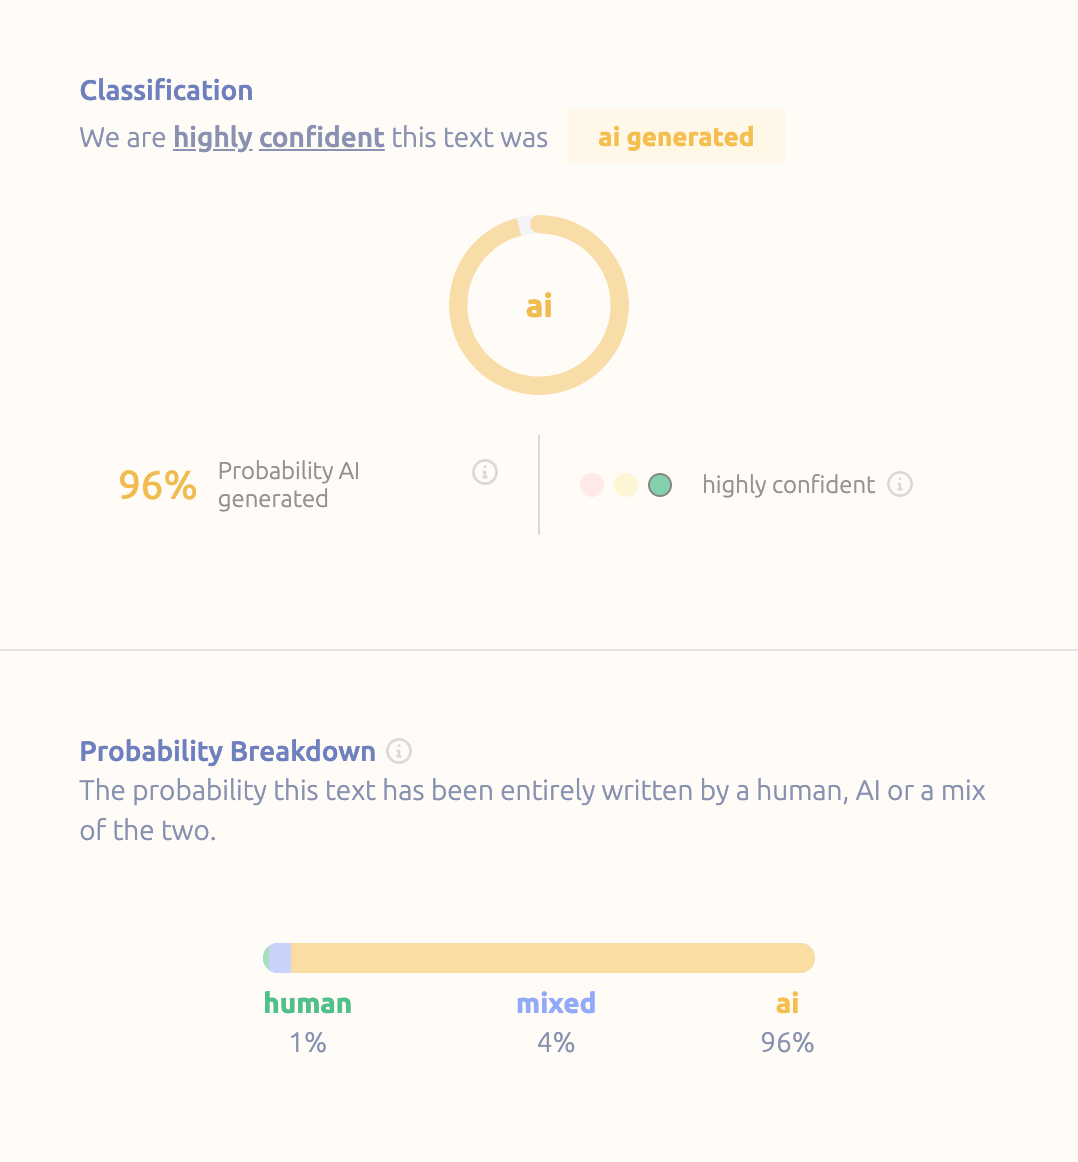
\includegraphics[width=\textwidth]{humbot2.png}
        \caption{GPTZero classification before using Humbot}
    \end{minipage}\hfill
    \begin{minipage}{0.45\textwidth}
        \centering
        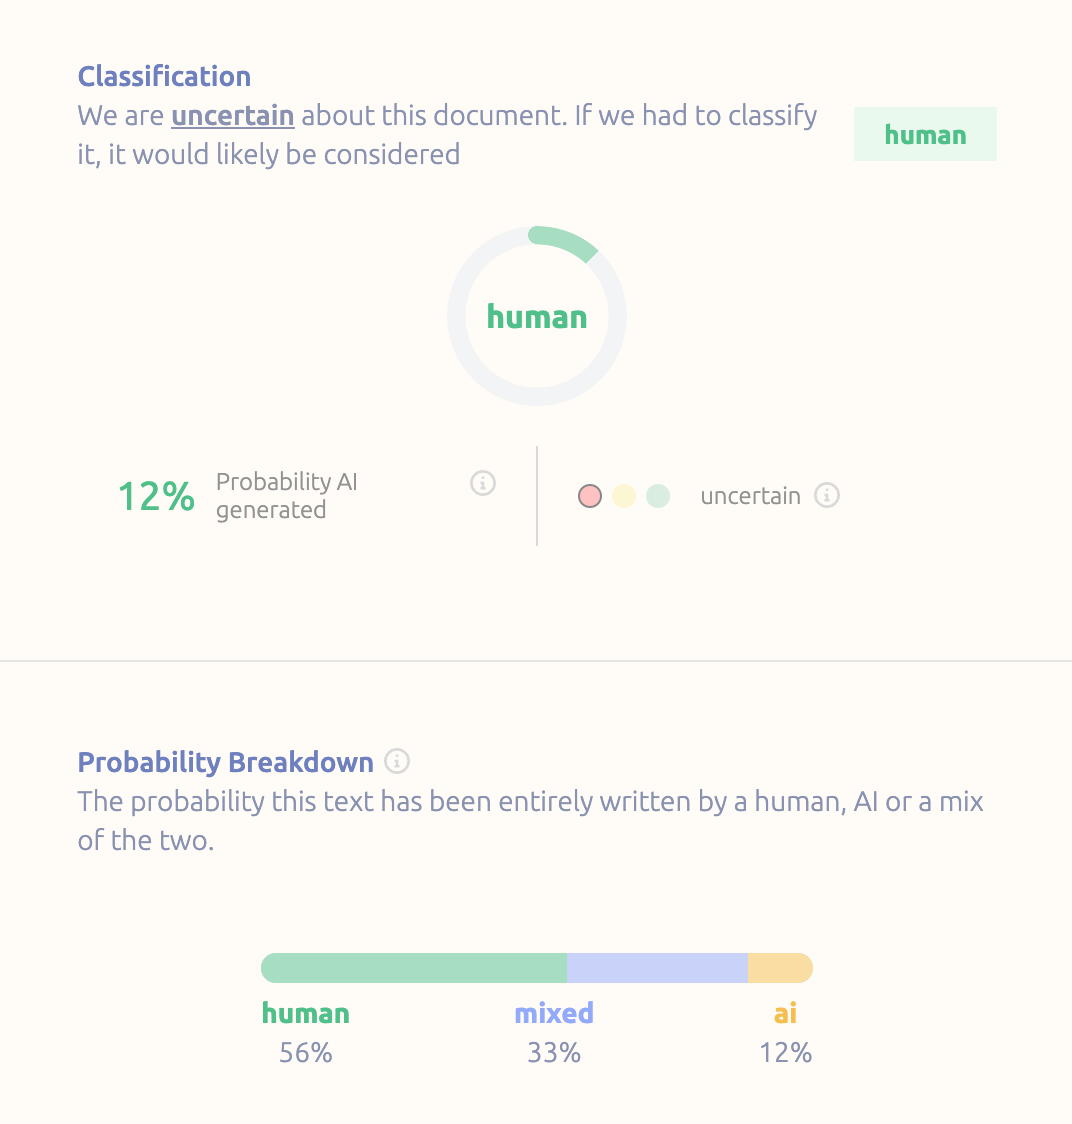
\includegraphics[width=\textwidth]{humbot1.png}
        \caption{Classification after using Humbot}
        \label{fig:humbotFig}
    \end{minipage}
\end{figure}

In the end, what we are seeing is an unsustainable arms race between ML GAI methods and ML detection methods, with GAI always one step ahead. ML detection methods will always be using old training data, and is working off the assumption that all GAI content will contain the same underlying patterns and giveaways. This is clearly an extremely bold claim to make, and even moreso is the assumption that there will always be some level of underlying pattern to detect.

\section{Objectives \& Design}
\subsection{Initial Design Ideas}
Initially, to circumvent the extensive issues with direct detection detailed previously, but to still allow for seamless and automatic verification, HumanMade was to work on an `evidence collection' basis. Evidence relating to the creative process itself would be collected, with the hope that this would give enough of a holistic input to whatever (likely ML) model was being used to decide whether a creation was human or AI generated. Upon starting the project, there were some large caveats with this approach:
\subsubsection{Issues}
\begin{itemize}
    \item Data collection for training would be long \& an unproductive use of time. There were no existing datasets for my purpose.
    \item Data collected would be messy, with few consistent patterns. `Evidence' could have included screen recordings, screenshots, timelapses, etc. There would not have been many consistent underlying features or patterns to learn to make a fully automated ML approach work well.
    \item Not actually avoiding the fundamental issues stemming from direct detection. At some point, GAI technologies would probably get so good that they would be able to generate the evidence being used to identify human made creations. This leads to a further philosophical point detailed later.
\end{itemize}
It was clear a more holistic approach would be required, one that speaks to the subjectivity and philosophical nature of the problem. We want an approach that focuses on helping a consumer themselves decide if a creation has had enough human involvement to warrant supporting, and one that gives human creators a thriving community and the tooling to effectively share their work. Instead of trying to crack the problem head on, which research and analysis of the industry indicated is probably futile anyway, we try instead to provide a platform which makes it cumbersome and infeasible to share and pass off purely AI generated works as human creations in the first place.
\subsection{Final Design}
After adequate research and analysis of the industry, the final design for HumanMade revolves around the idea of a progress timeline for each creation, consisting of `commits' representing chunks of progress.
\begin{itemize}
    \item Each creator-defined commit will consist of files, a description, a percentage of completion, and an icon to denote whether an AI tool was used.
    \item Each of these commits will have the option to be tamper-proofed and traceable to the original creator. In a world inundated with synthetic art, it could be the case that authentic human made art becomes a scarce or highly valued commodity, in which case there are incentives to ensure creations remain verifiable to a particular user and origin date. 
    \item The progress timeline will be tested for continuity and progression that makes `sense' for a human creator, helping human creators prove the legitimacy of their creations to consumers.
    \item Each creation, once completed, can be added to a Marketplace to be viewed by everyone.
\end{itemize}

\subsubsection{Advantages}
This final design lends itself well to avoiding the issues we discussed in Initial Design Ideas, and aligns with the final point made in the Issues section about the importance of a holistic approach.
\begin{itemize}
    \item Generative AI has a very obvious `diffusion' progression. An image of pure noise is slowly transformed into the final output. This would be easy to spot on a progress timeline, and be picked up by our image similarity techniques.
    \item The approach allows the community to decide the level of AI involvement that they are comfortable with in a creation, as this is clearly a gray area. Certain AI tools which simply help a human creator be more effective in translating their creative ideas may not be inherently negative.
    \item The approach sidesteps the `arms race' between AI detectors and AI generators by allowing the community to decide for themselves what they think constitutes a human made creation. At a philosophical level, the best `neural network' one can use to achieve the aims of human made is the human brain.
    \begin{figure}[H]
        \centering
        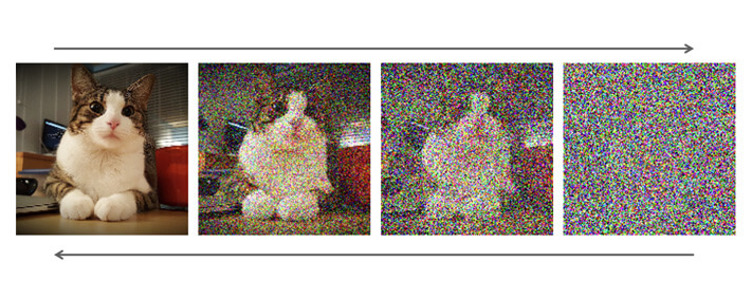
\includegraphics[scale=0.3]{catDiffusion.jpg}
        \caption{An example of the diffusion progression when generating a photo of a cat \cite{cat}.}
    \end{figure}
\end{itemize}




\noindent Now that we have specified the general design for HumanMade, we look into Objectives of the project. We start with the core, fixed objectives. These consist of `Must' and `Should' have priority objectives.
\subsection{Fixed objectives}
\subsubsection{Functional objectives}
\begin{itemize}
        \item There must be a simple login/signup page, where a user can authenticate themselves securely with the application via email.
        \item There must be Creations page, which allows a user to view their existing creations once authenticated, and to add a new creation. A user should be able to specify a title, a type and a description for the creation.
        \item There must be custom page for each creation, containing the progress timeline of the creation. A user should be able to add commits to the timeline via an intuitive UI, and there should be an option to complete the creation.
        \item There must be a Marketplace page, which allows a user to view, like and filter finished creations from other creators. Once a user completes a creation, it will be listed to the Marketplace.
        \item The app should make use of machine learning techniques to analyze the continuity of a progress timeline.
        \item The app should provide a way to make a commit tamper-proof and traceable to a specific user.
\end{itemize}
\subsubsection{Nonfunctional objectives}
These are quality attributes that the system should have:
\begin{itemize}
    \item Every page should load within under a second. The probability of bounce (a user leaving the page before interacting) increases 32\% as load times go from 1 to 3 seconds \cite{googleload}.
    \item The web app must be user-friendly, intuitive, and conform to WCAG accessibility guidelines. It must be reactive and take advantage of modern web development technologies which improve performance and maintain correctness. 
    \item All services used in HumanMade, third-party or self-developed, should make use of scalable and performant technologies, and if third-party they should be reliable and fault-tolerant.
    \item The entire HumanMade system should stress modularity. This can be achieved through the use of a microservices architecture, and communication between disparate services should take place with well-defined REST (or another popular standard) APIs. 
    \item The HumanMade system should stress portability. Since the main interface users will use to communicate with HumanMade will be a web application, any internet enabled device with a modern browser will support the platform. However we should ensure that extra features like tamper-proofing and traceability, or the command line interface, are accessible from all popular operating systems and enivronments.
\end{itemize}

\noindent Flexible objectives are non-essential to the success of the platform as a proof-of-concept, but would add to the user experience and improve the service. These are `Could have' priority objectives.
\subsection{Flexible objectives}
\begin{itemize}
    \item The login/signup Homepage could be fleshed out further to involve user profiles
    \item We could implement a command line interface for easy publishing to the progress timeline for creatives, instead of having to go through the web app UI.
\end{itemize}
Finally, we touch on objectives which could be part of the platform but are to be avoided as a way of managing the scope of the project. 
\subsection{Avoidable objectives}
\begin{itemize}
    \item We will avoid implementing following/follower functionality. This would allow for creators to build a loyal audience and brand and for consumers to stay up-to-date with a creators latest creations, however this would greatly increase the scope of the project and would likely not be contributing any new concepts in terms of implementation details.
    \item We will avoid implementing the ability to purchase the artwork associated with a creation on the Marketplace. Again, this would greatly increase the scope of the project without being exploratory in any way.
\end{itemize}

\section{Functionality}
There are then four main areas of development:
\begin{enumerate}
    \item \textbf{Web App} \\This involves giving users the ability to make new creations, commit to and view their progress timeline for each creation, and a marketplace for finished creations. This is the main interface that creatives and consumers will be using to interact with HumanMade.
    \item \textbf{Machine Learning Microservice} \\This is a key component for implementing the continuity testing alluded to in the Final Design chapter. A metric for the continuity and progression across commits is computed using ML techniques, and then displayed on the progress timeline in the web app UI.
    \item \textbf{Blockchain Interface} \\This provides a simple interface to make any commit tamper-proof and traceable by allowing users to record their commits to the blockchain. Specifically, files contained in a commit and the user's ID are hashed together and recorded on the chain. Now, trivially the commit is traceable to the original user, and is tamper-proof as if the files in the commit are changed at all, the hashes can be checked and will no longer line up with the ones stored on the chain. The blockchain interface is a separate, large area of development, but is tightly integrated within the web app.
    \item \textbf{Command Line Interface} \\This is a tool that allows creators to easily add commits to their progress timelines, hopefully reducing the effort it takes and avoiding interruption of the creative process.
\end{enumerate}
We will look at the completed functionality of each before delving into implementation details.
\subsection{Web App}
\subsubsection{Homepage}
\begin{figure}[H]
    \centering
    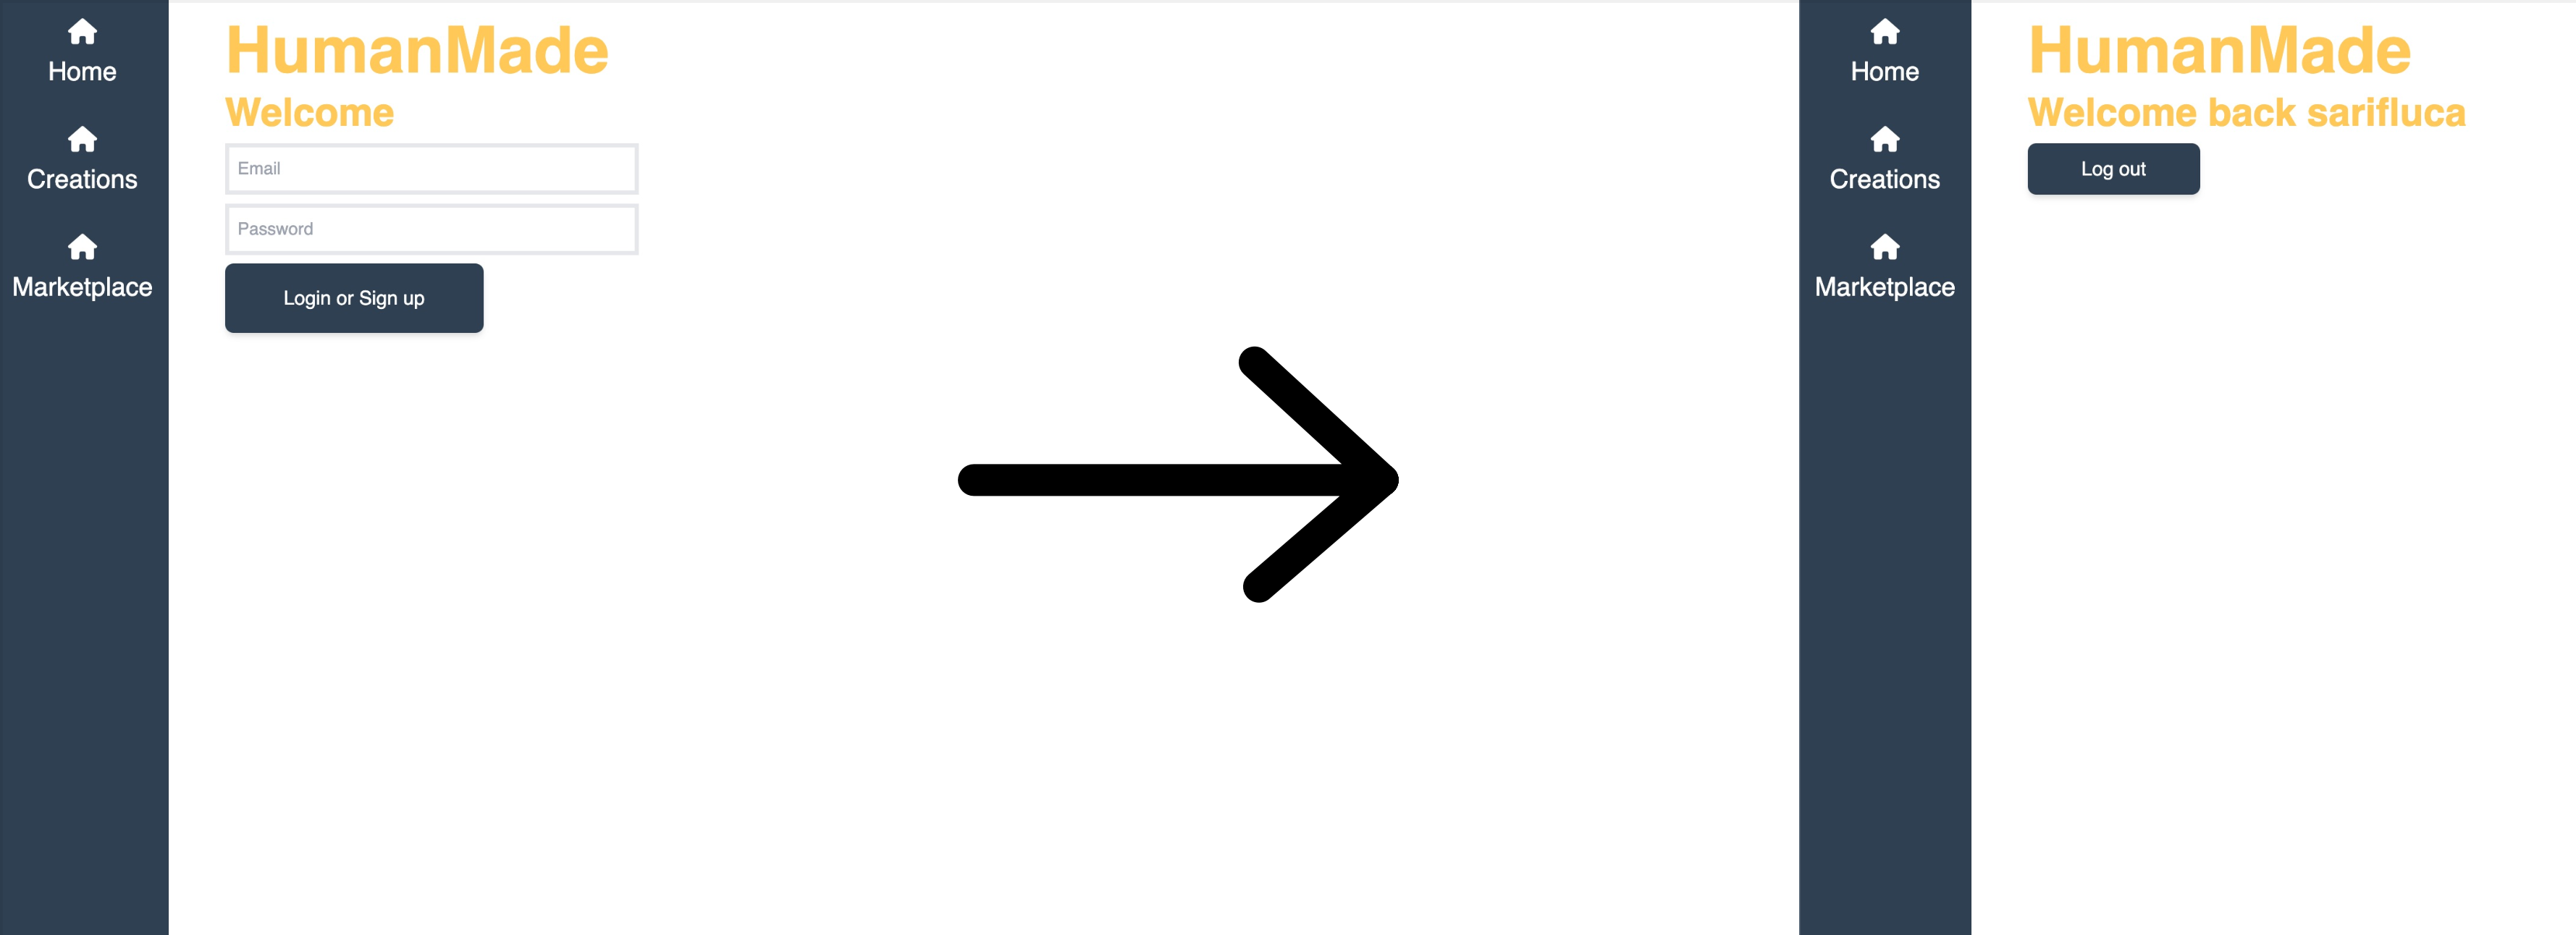
\includegraphics[scale=0.2]{login.png}
\end{figure}
There is a basic homepage, currently only serving login/sign up functionality. A user must sign up or login using their email, and the same interface is used for both for simplicity.
\subsubsection{Creations}
This is the tab of main importance in the application. Once a user is logged in, they will be greeted with any existing creations, and can create new creations.
\begin{figure}[H]
    \centering
    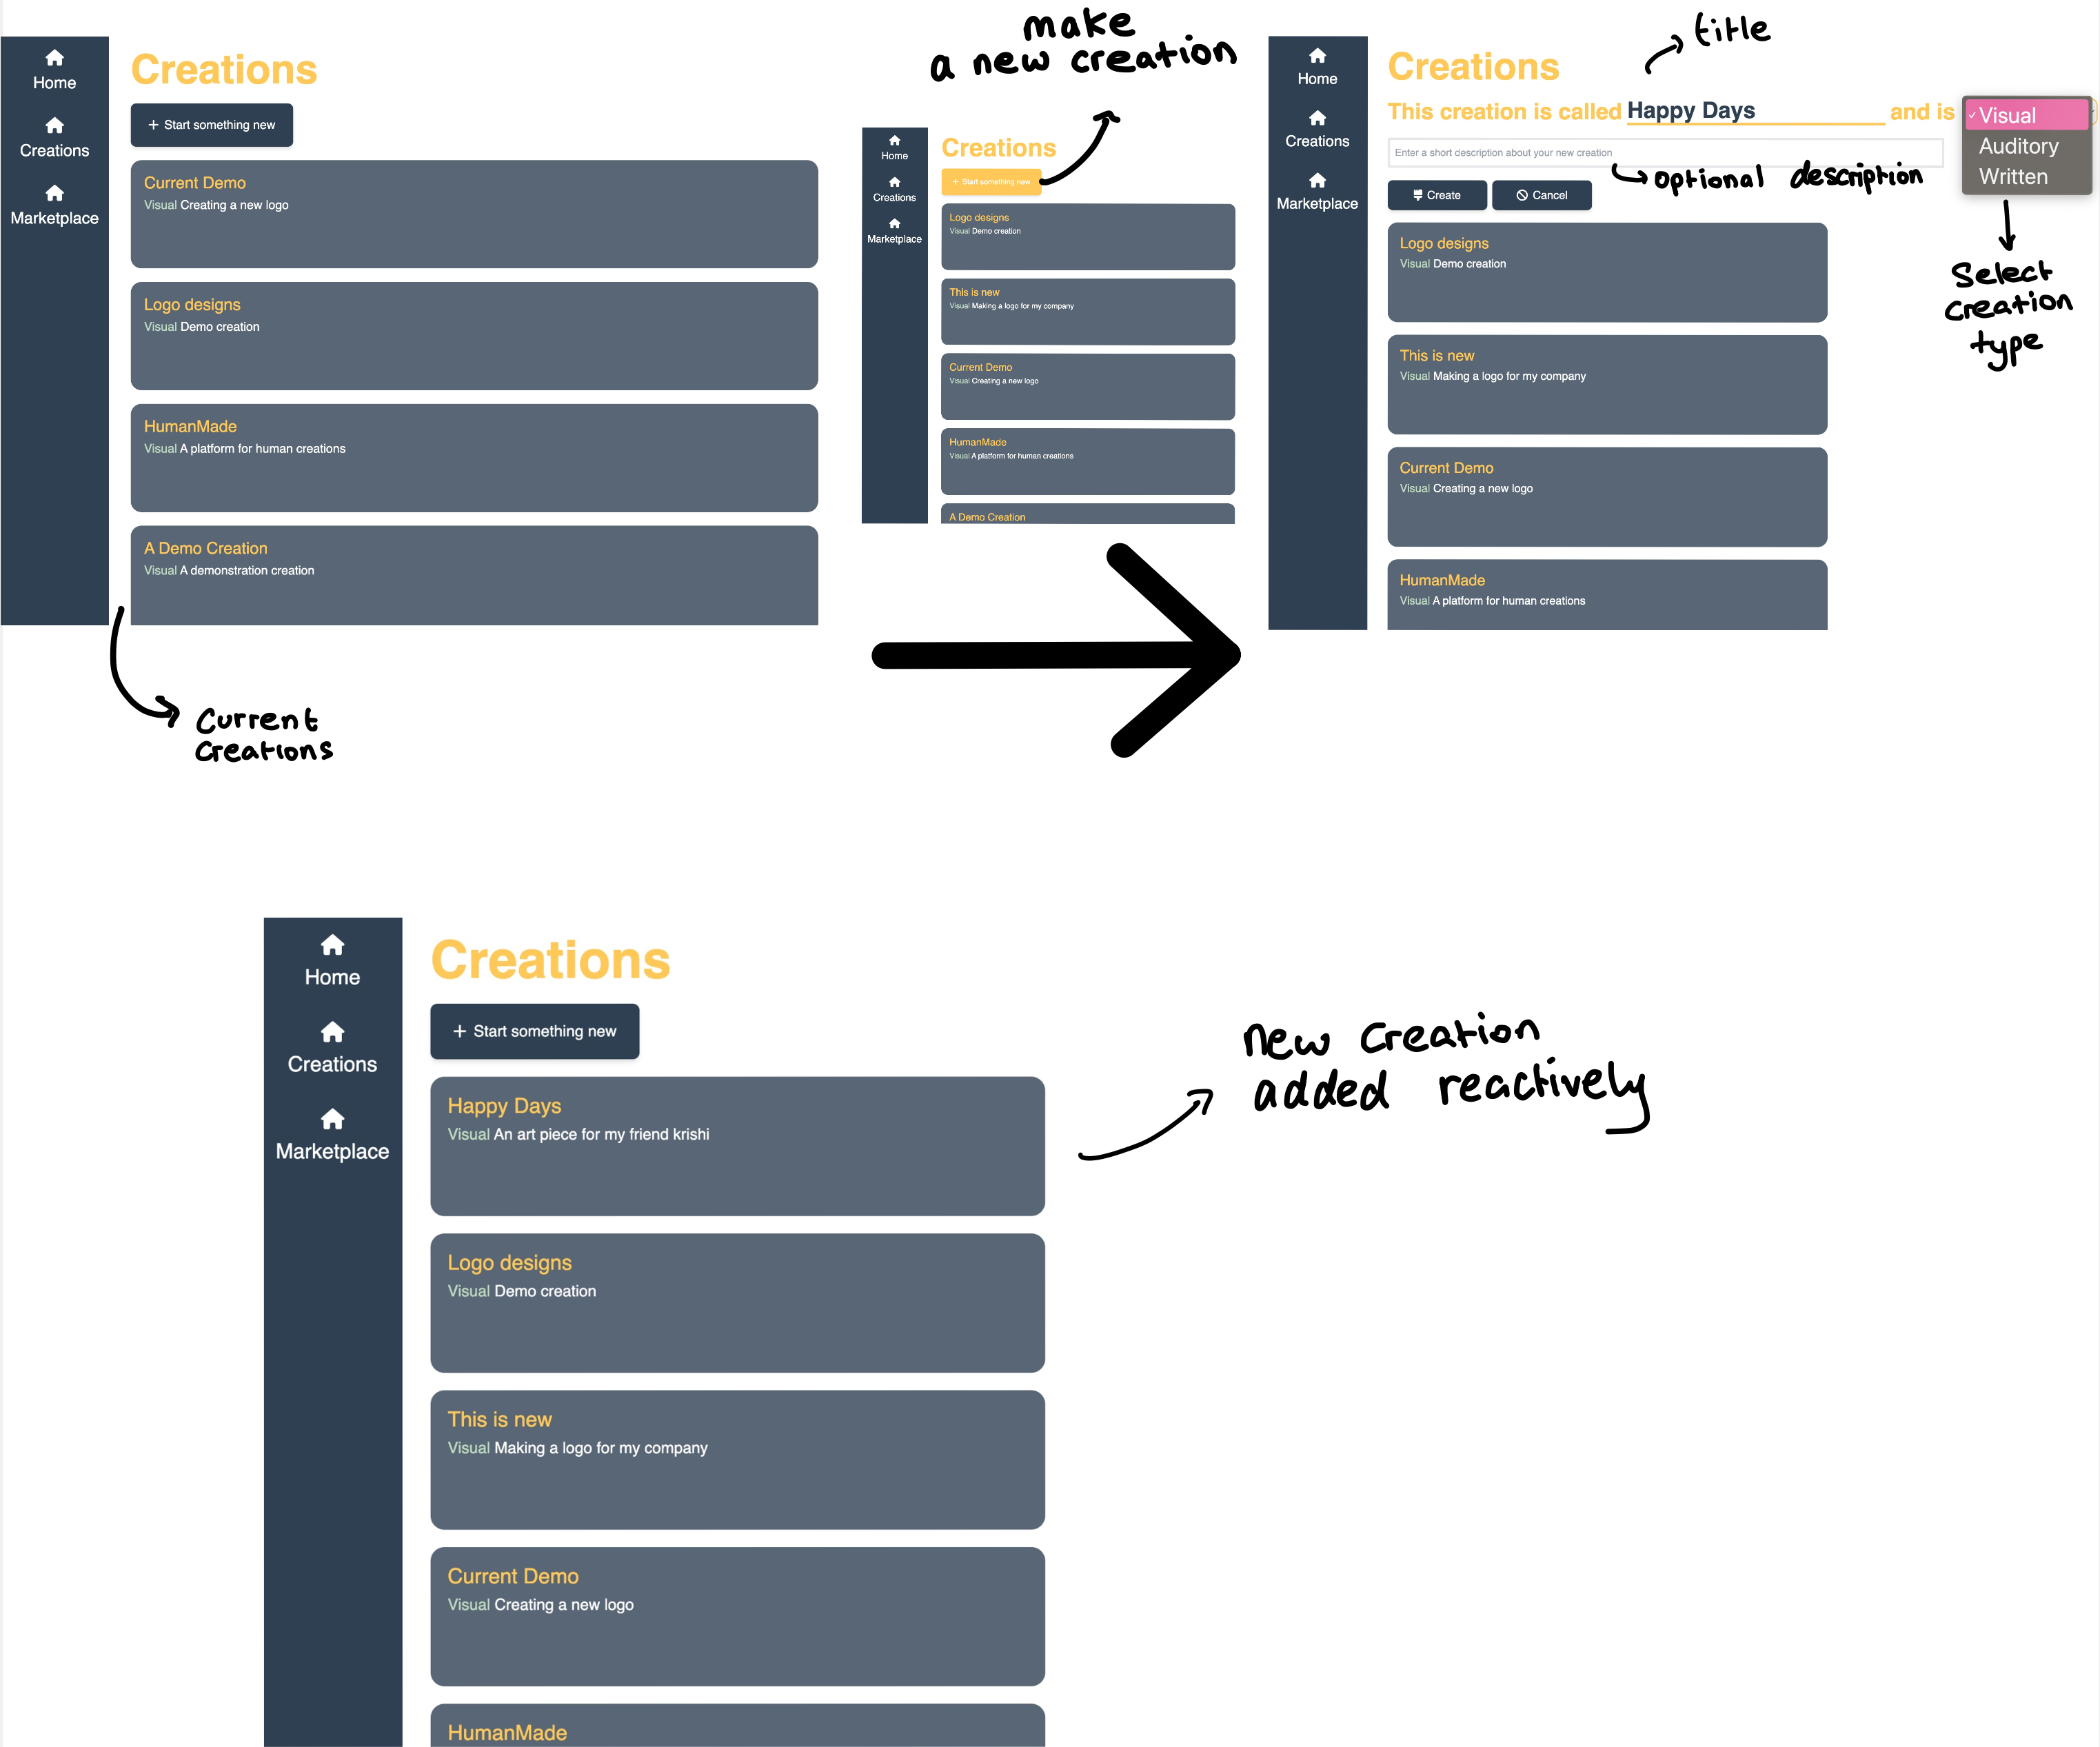
\includegraphics[scale=0.35]{creations.png}
\end{figure}
\noindent Here a new creation entitled `Happy Days' is being created, specified as a `Visual' creation. Once created, the creation will automatically reactively show up at the top of the existing creations list, which is always ordered by most recently visited creation. 

\begin{figure}[H]
    \centering
    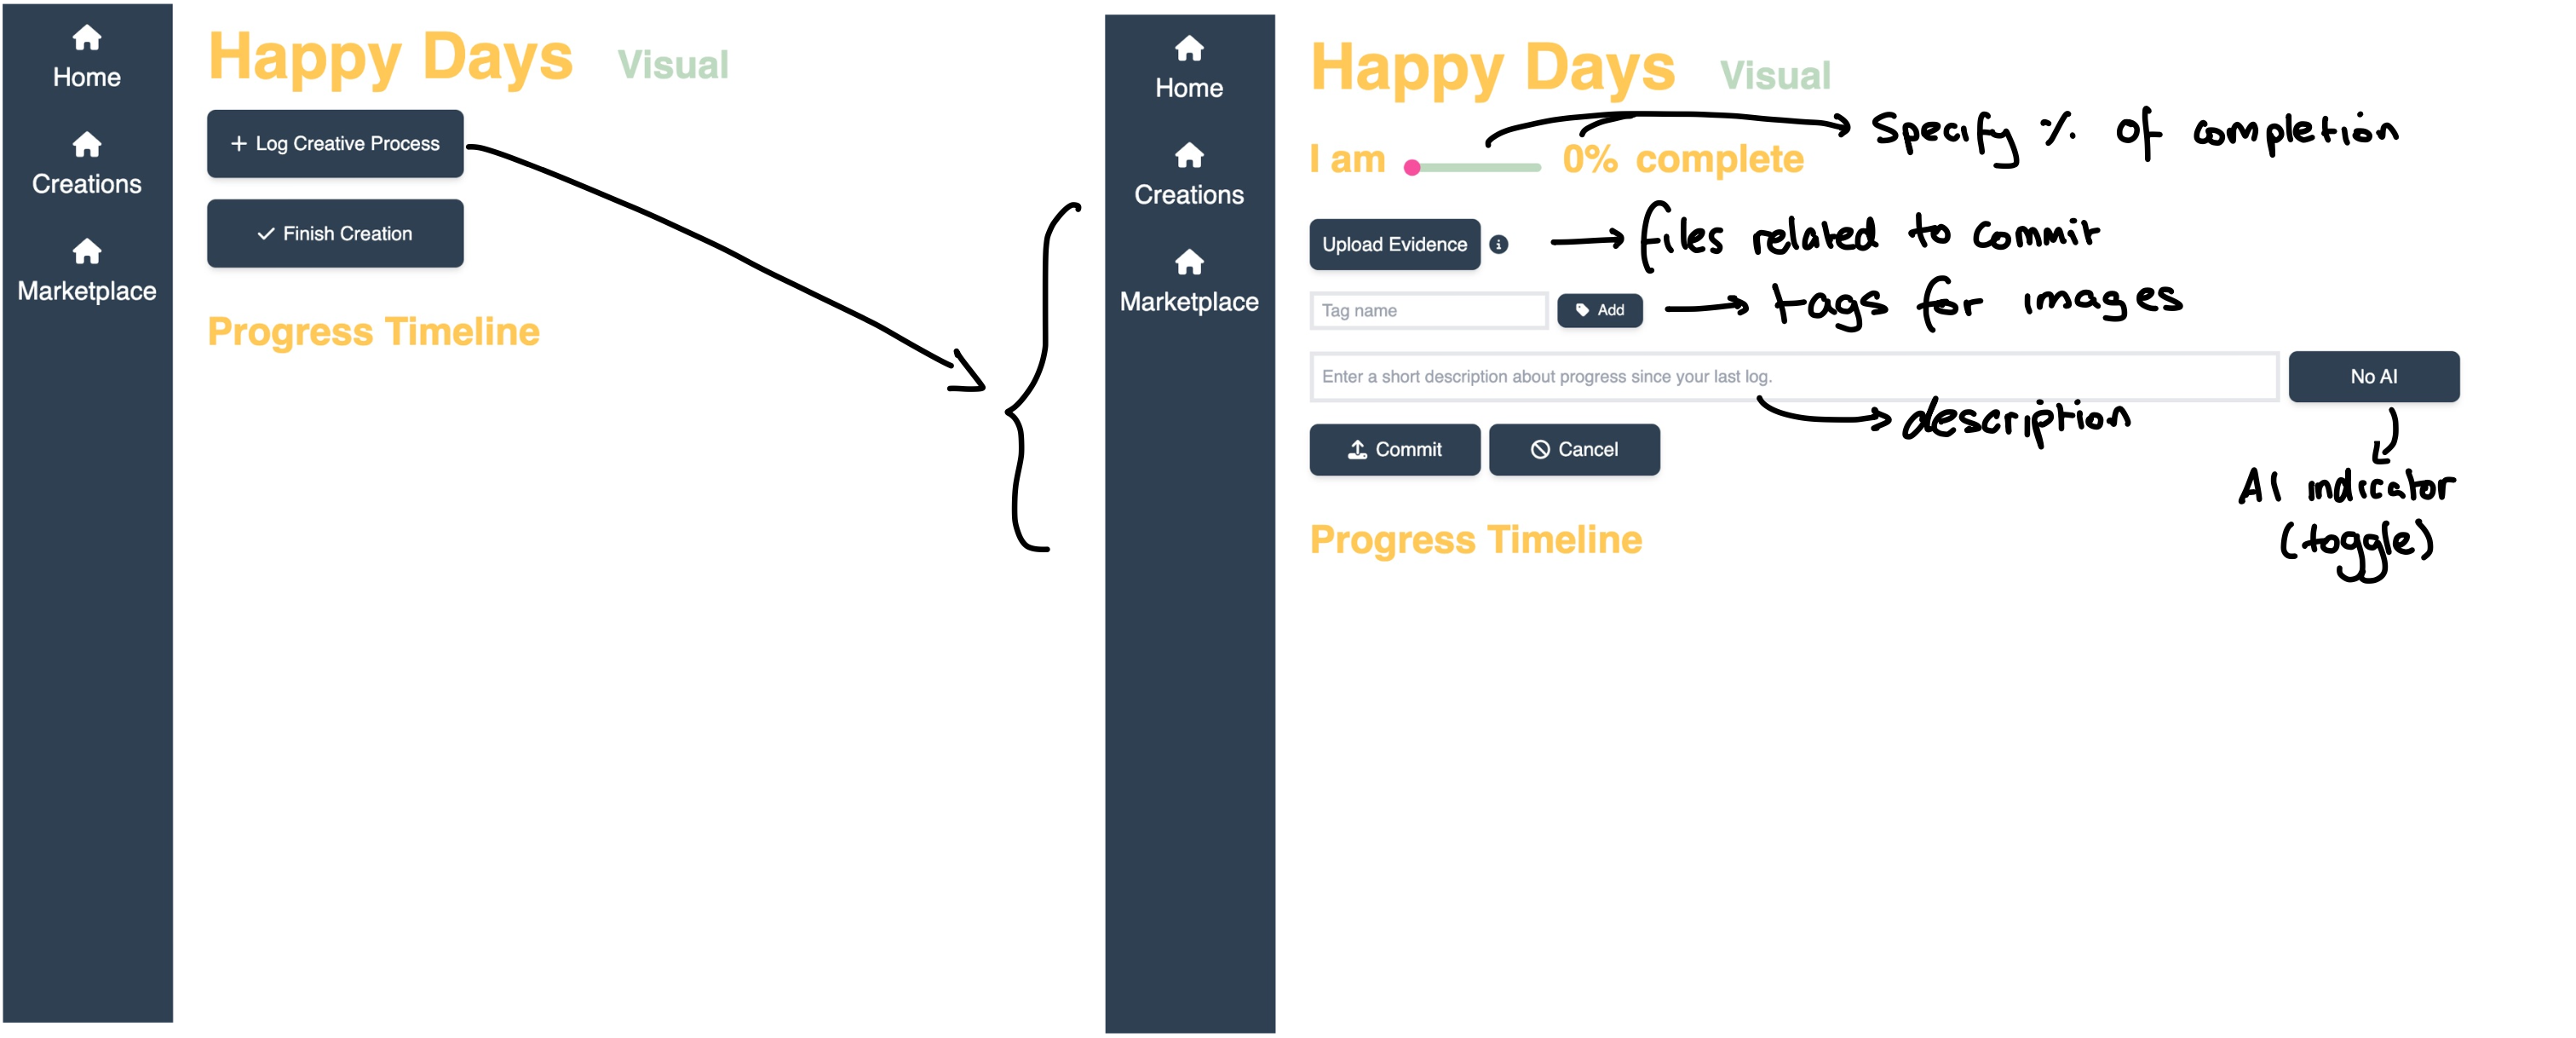
\includegraphics[scale=0.35]{creation.png}
\end{figure}

\noindent Clicking on the creation, we are greeted with it's progress timeline. Currently empty, we can commit to the progress timeline by clicking `Log Creative Process'. This opens up a slew of inputs to create the commit.


\begin{figure}[H]
    \centering
    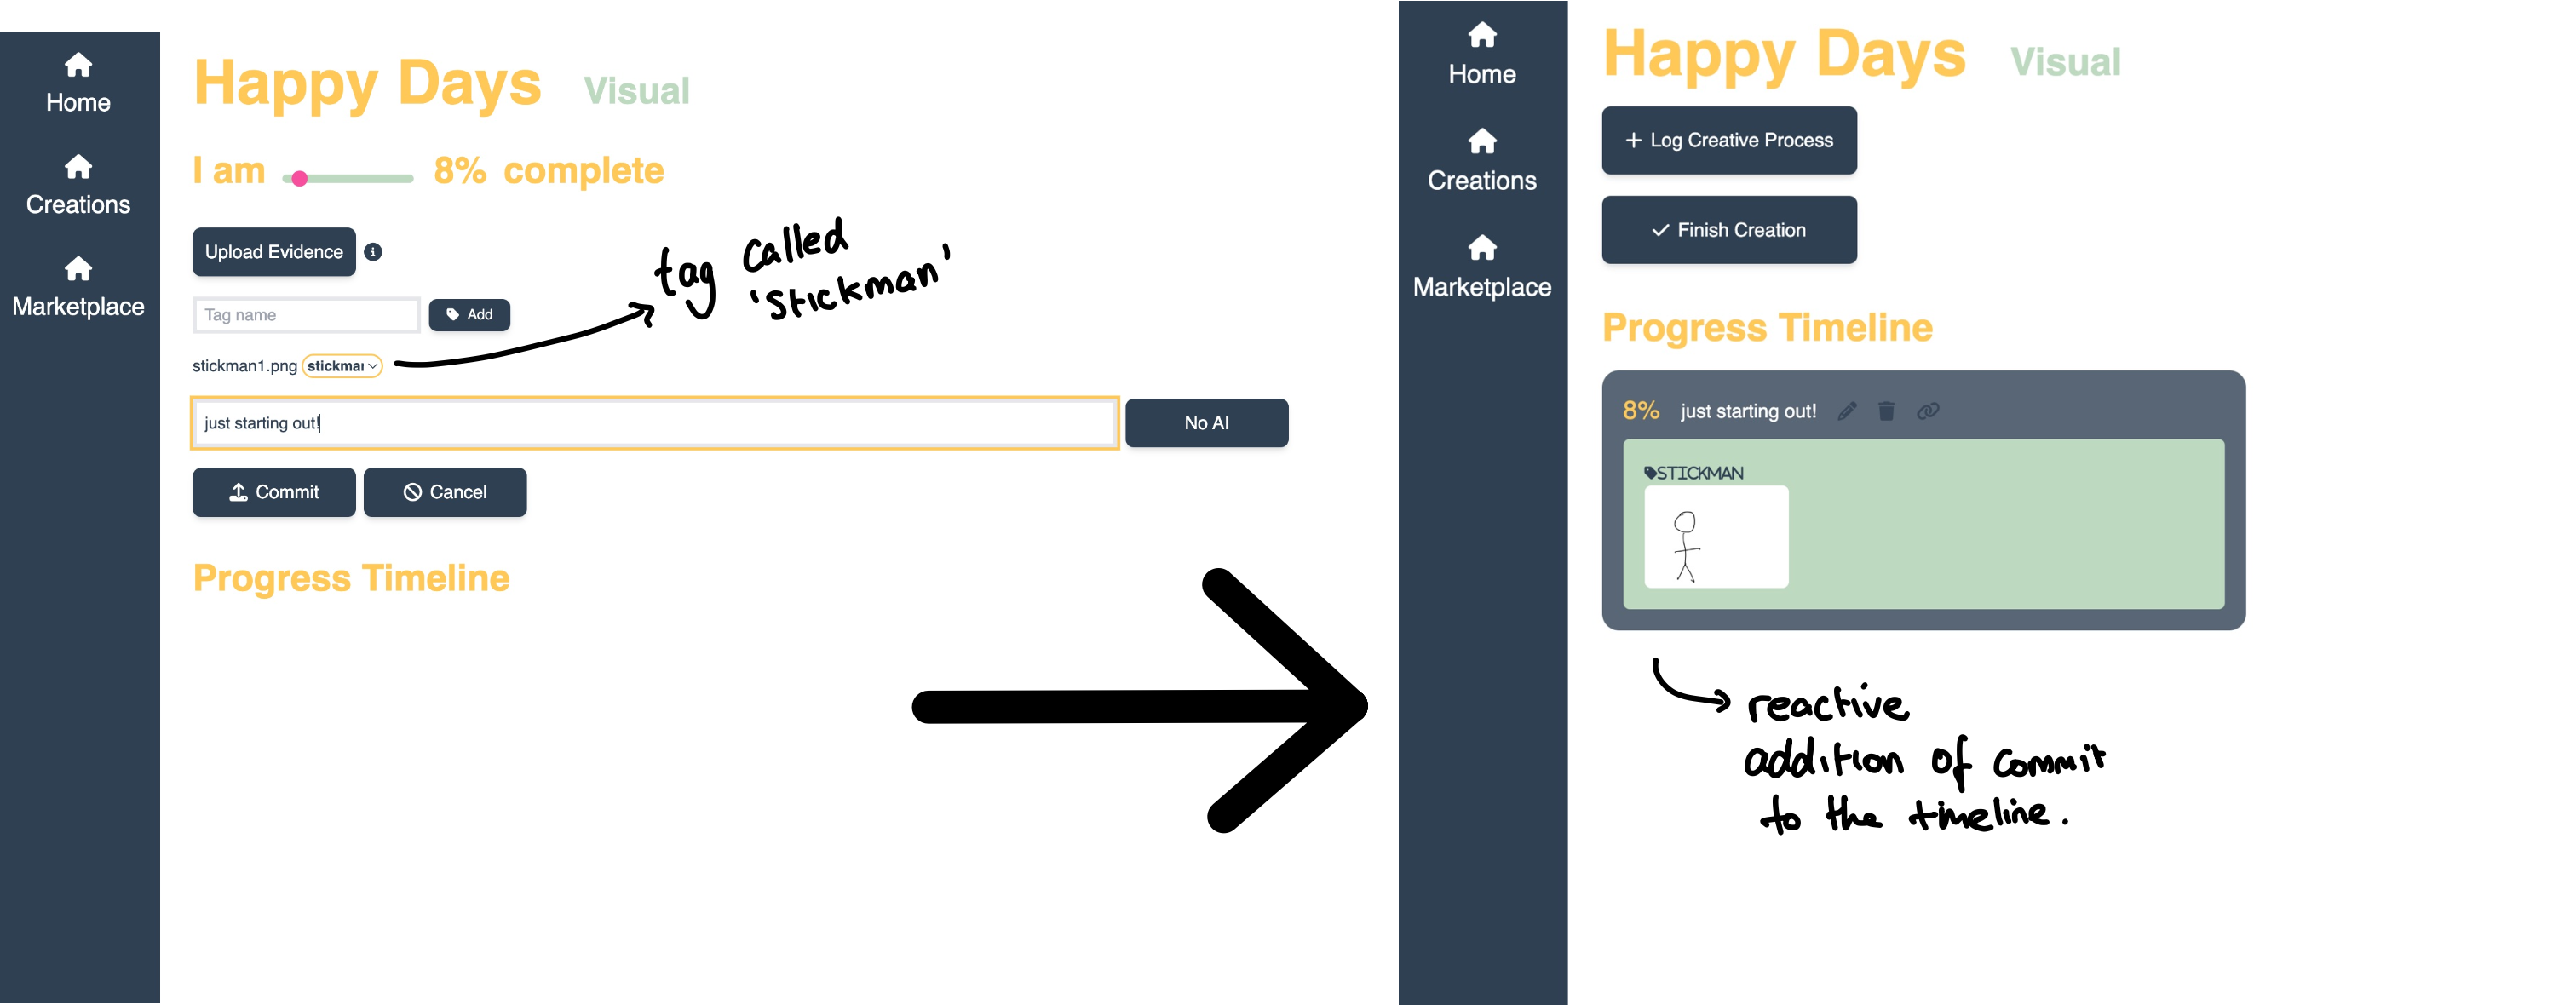
\includegraphics[scale=0.35]{tagging1.png}
\end{figure}
\noindent\textbf{Tagging:} A user can add tags to images in a commit. When the same tag is used for images across commits, the images are compared and a `similarity score' is computed. If the images do not correspond to a reasonable progression then this is marked on the progress timeline. This is how the ML microservice tests the continuity of a timeline, and we will go into further detail in the implementation chapter.\\\\Above, we add a new tag `stickman', and label the one image in our first commit with it. The commit reactively shows up on the progress timeline as soon as the commit goes through to the database. 

\begin{figure}[H]
    \centering
    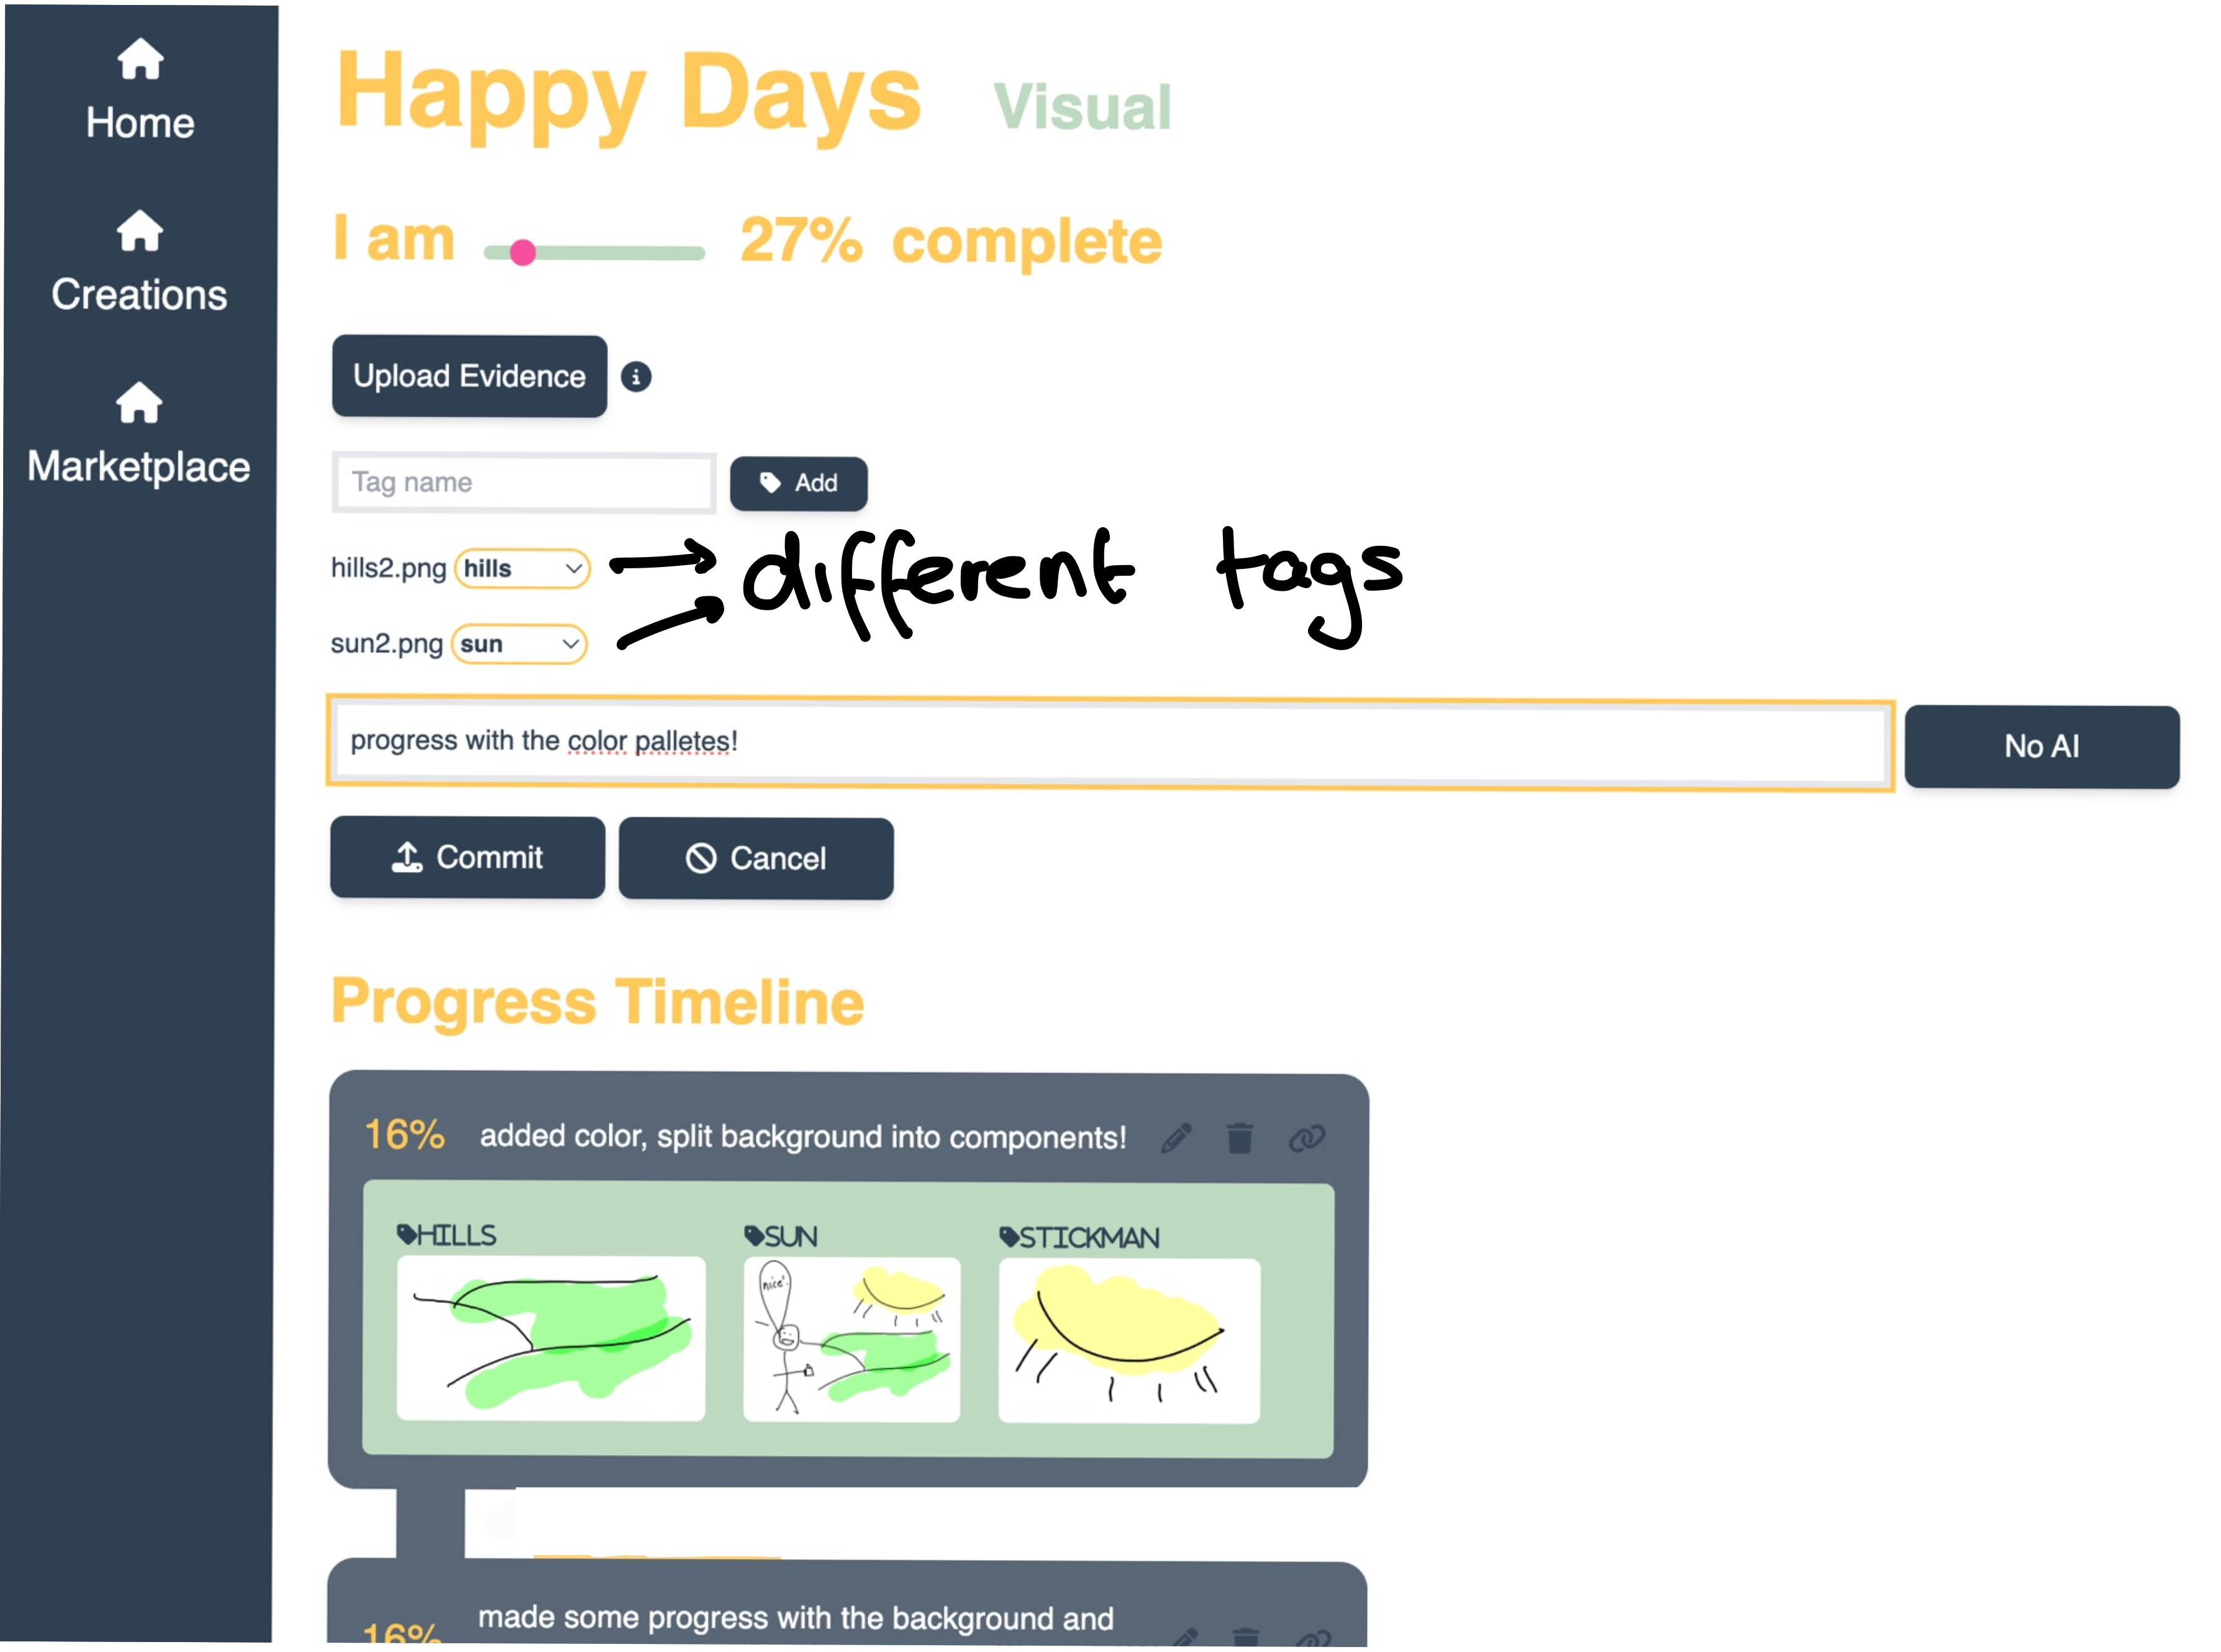
\includegraphics[scale=0.24]{tagging2.png}
\end{figure}
\noindent Further commits can be made with different tags, or the same tags to signal progression of an image across commits. A commit can of course contain multiple files of any kind. 

\begin{figure}[H]
    \centering
    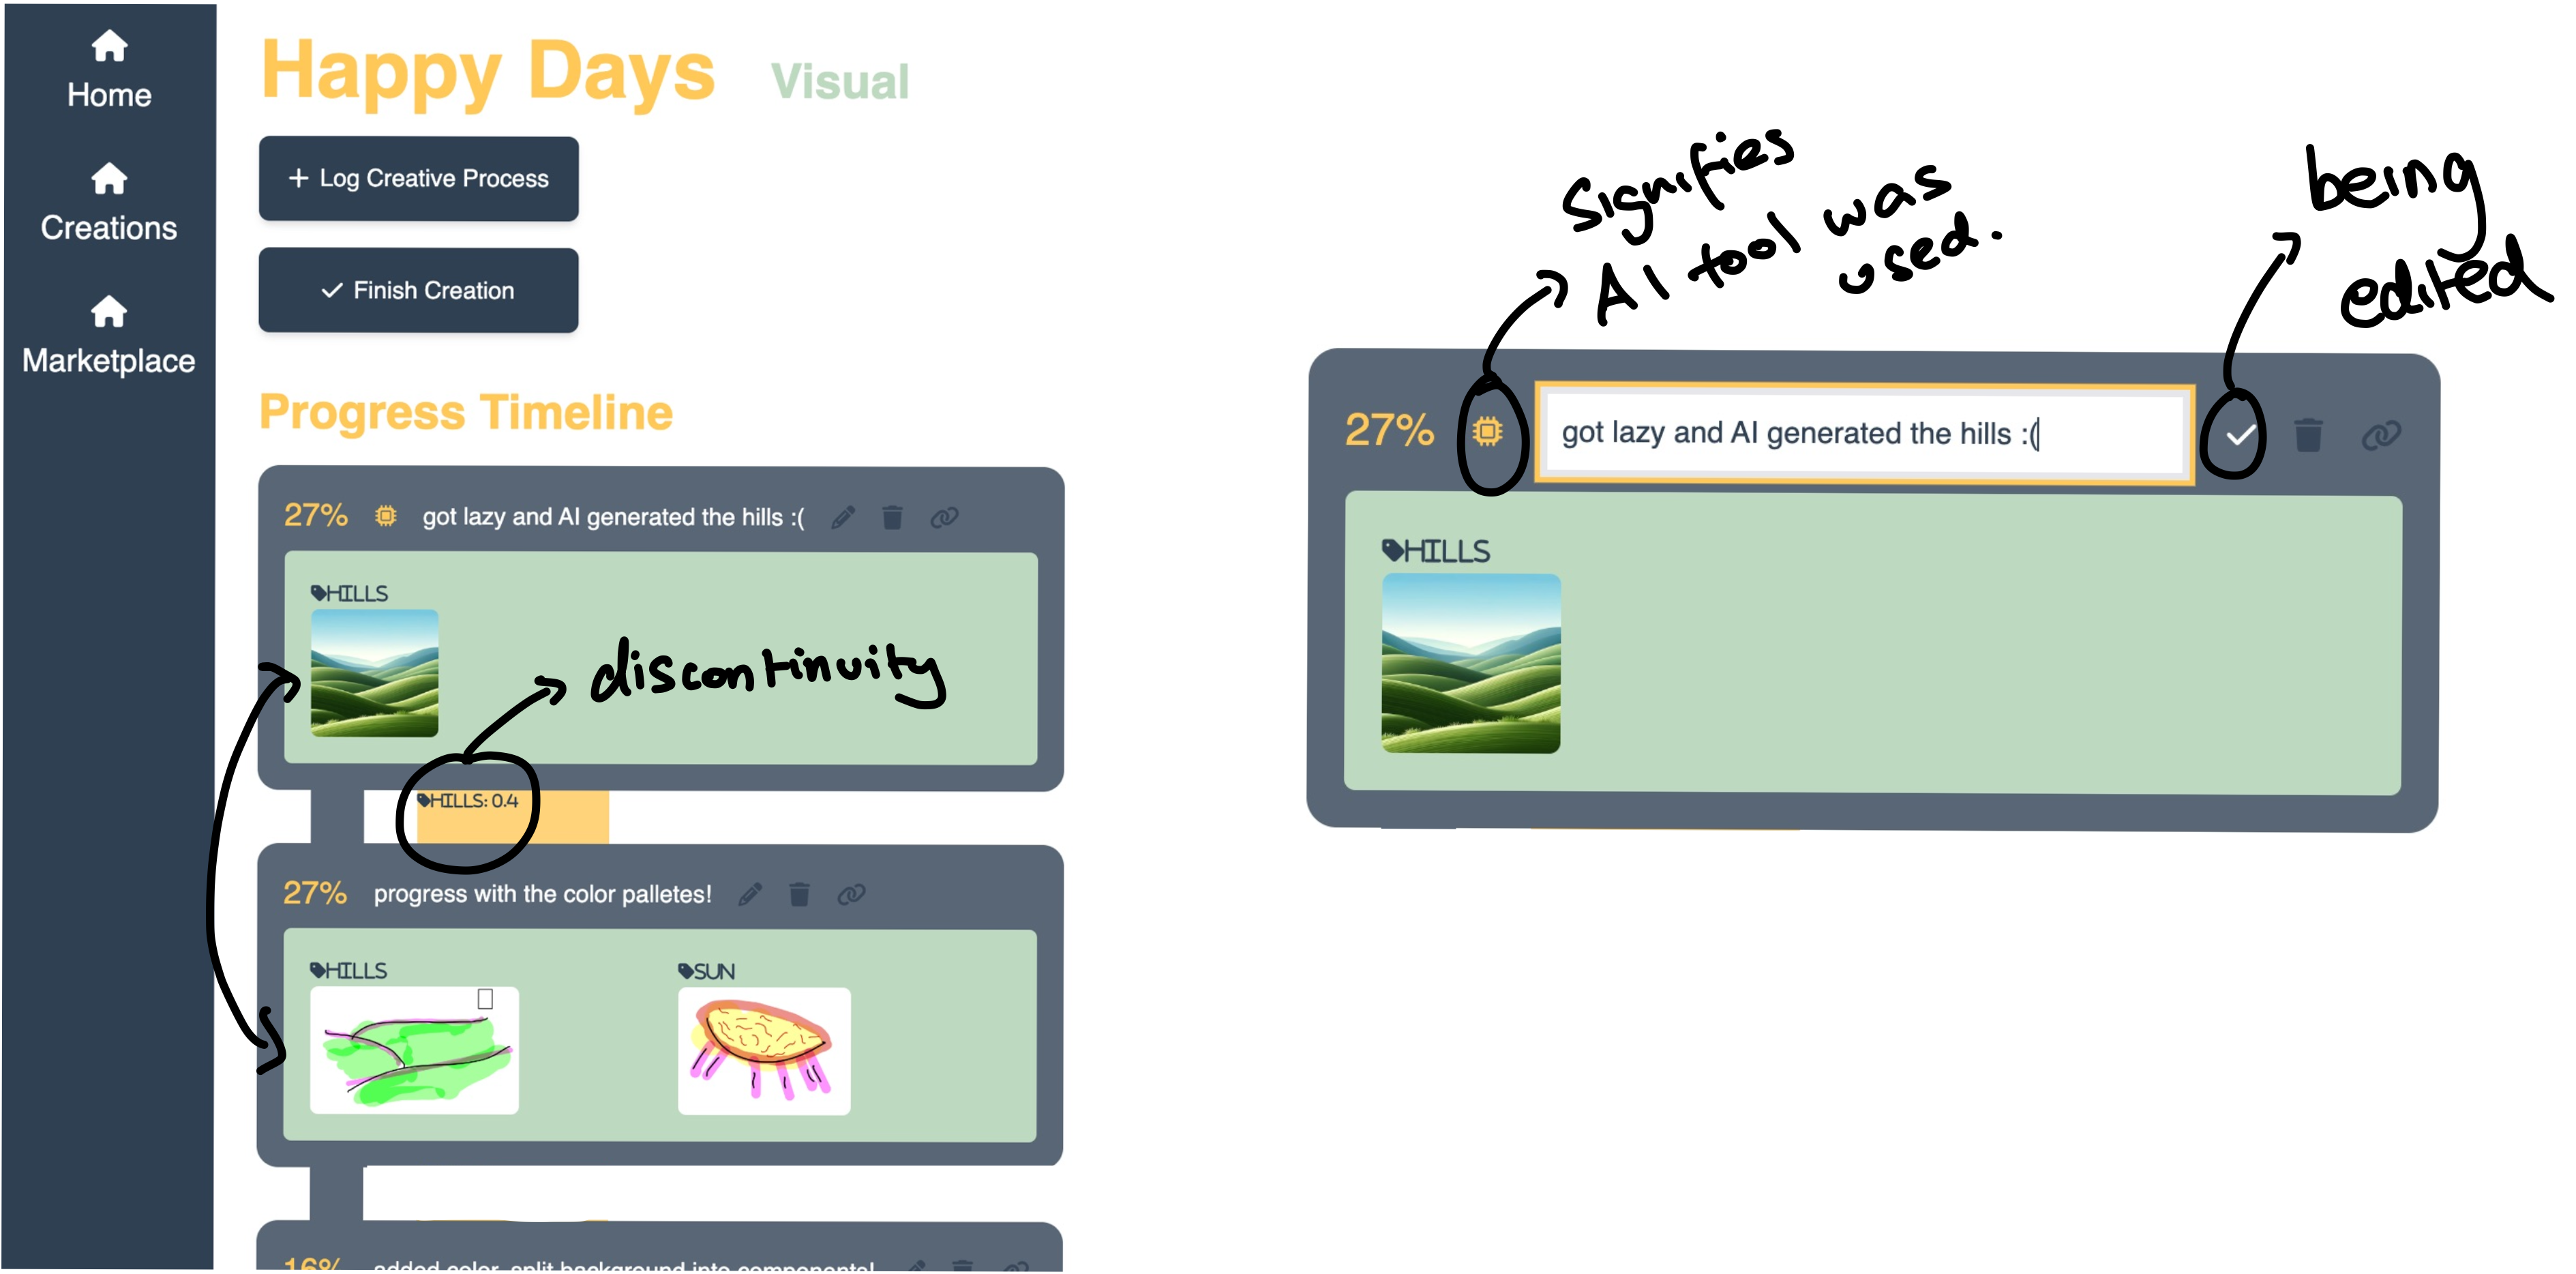
\includegraphics[scale=0.27]{tagging3.png}
\end{figure}
\noindent At one point we decide to AI generate our image of `hills', choosing to be transparent about the use of AI shown by the processor icon. However, our method for computing progression between commits alerts us (and later on any consumers who will be viewing this progress timeline when the creation is finished) that there is indeed an issue with the continuity between these two commits. It tells us that the two images marked `HILLS' only have a similarity score of 0.4. Also shown is ability to edit a commit description, synced reactively.
\begin{figure}[H]
    \centering
    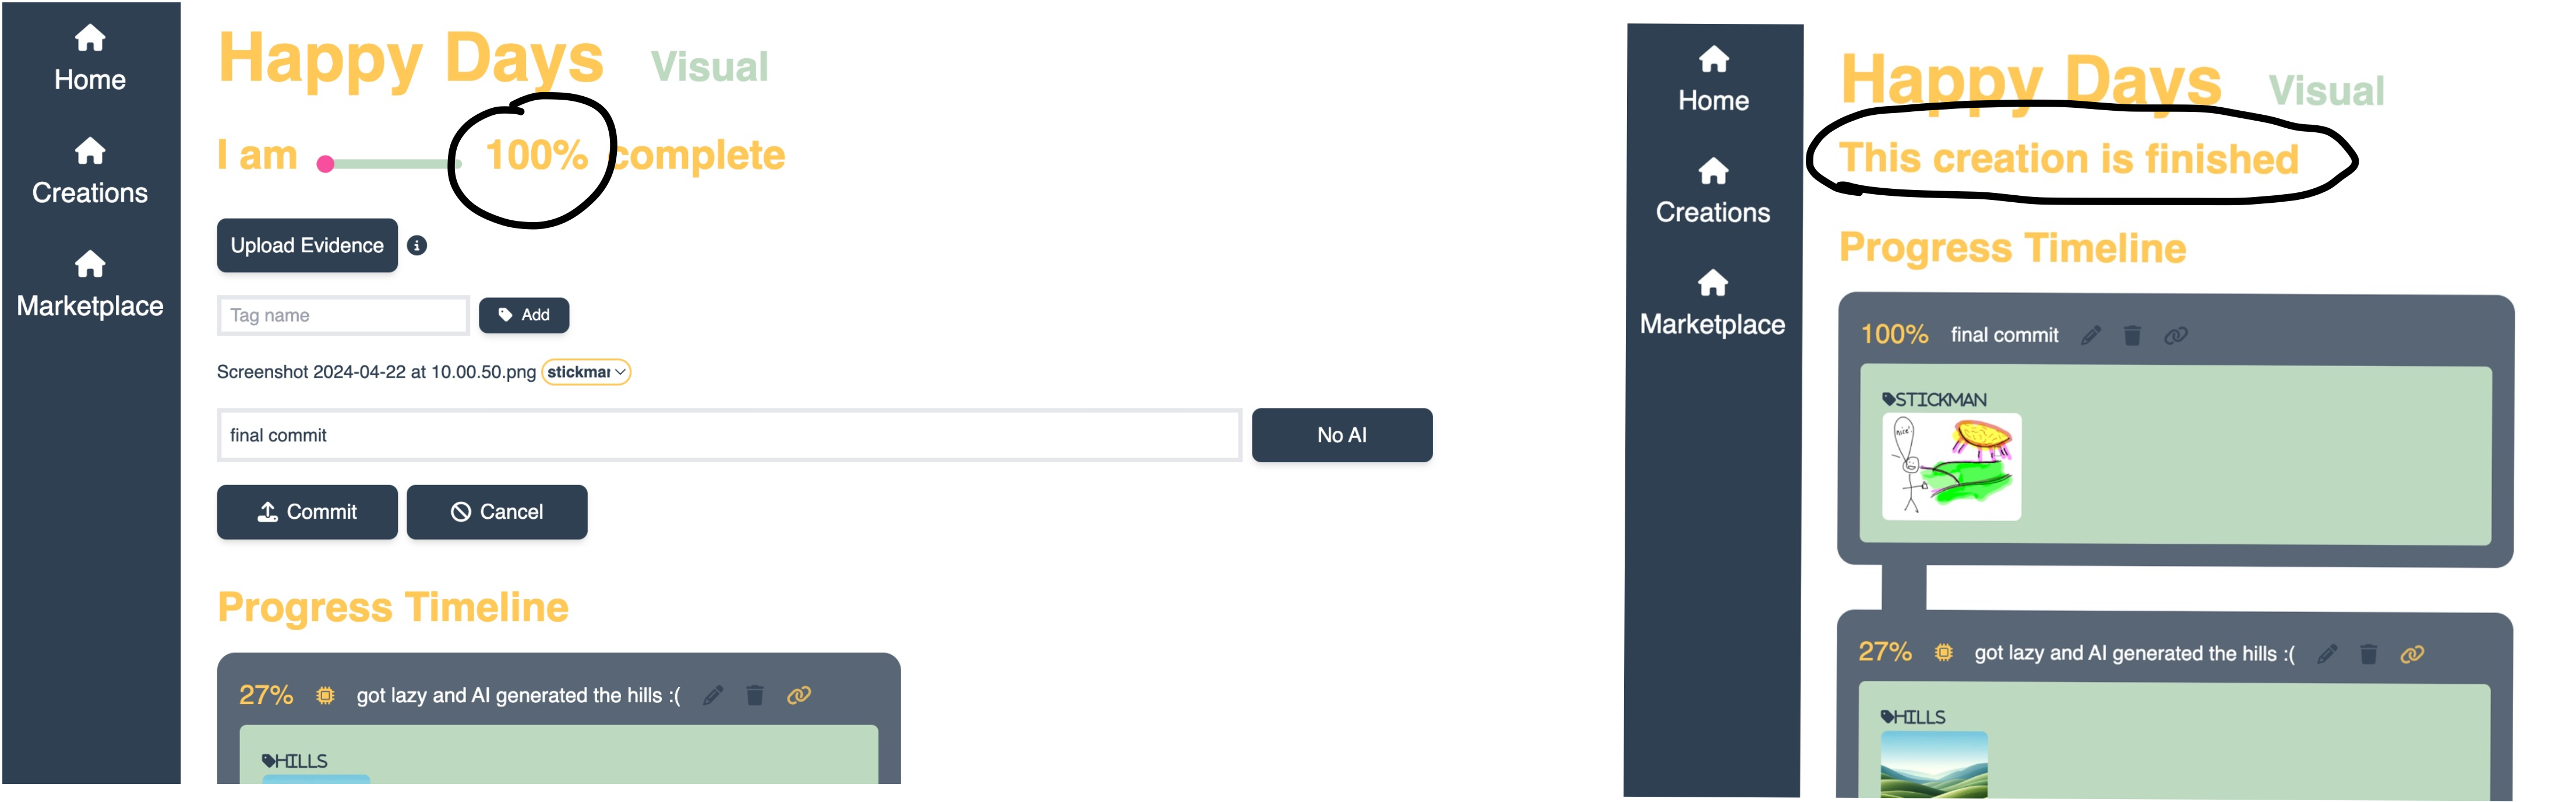
\includegraphics[scale=0.23]{finished.png}
\end{figure}
\noindent We finish by clicking `Finish Creation', which will bring up an option to submit a final commit of 100\% completion. Once this commit has been added, the creation is finished and the progress timeline can no longer be edited. The creation is then added to the Marketplace.


\subsubsection{Marketplace}
\begin{figure}[H]
    \centering
    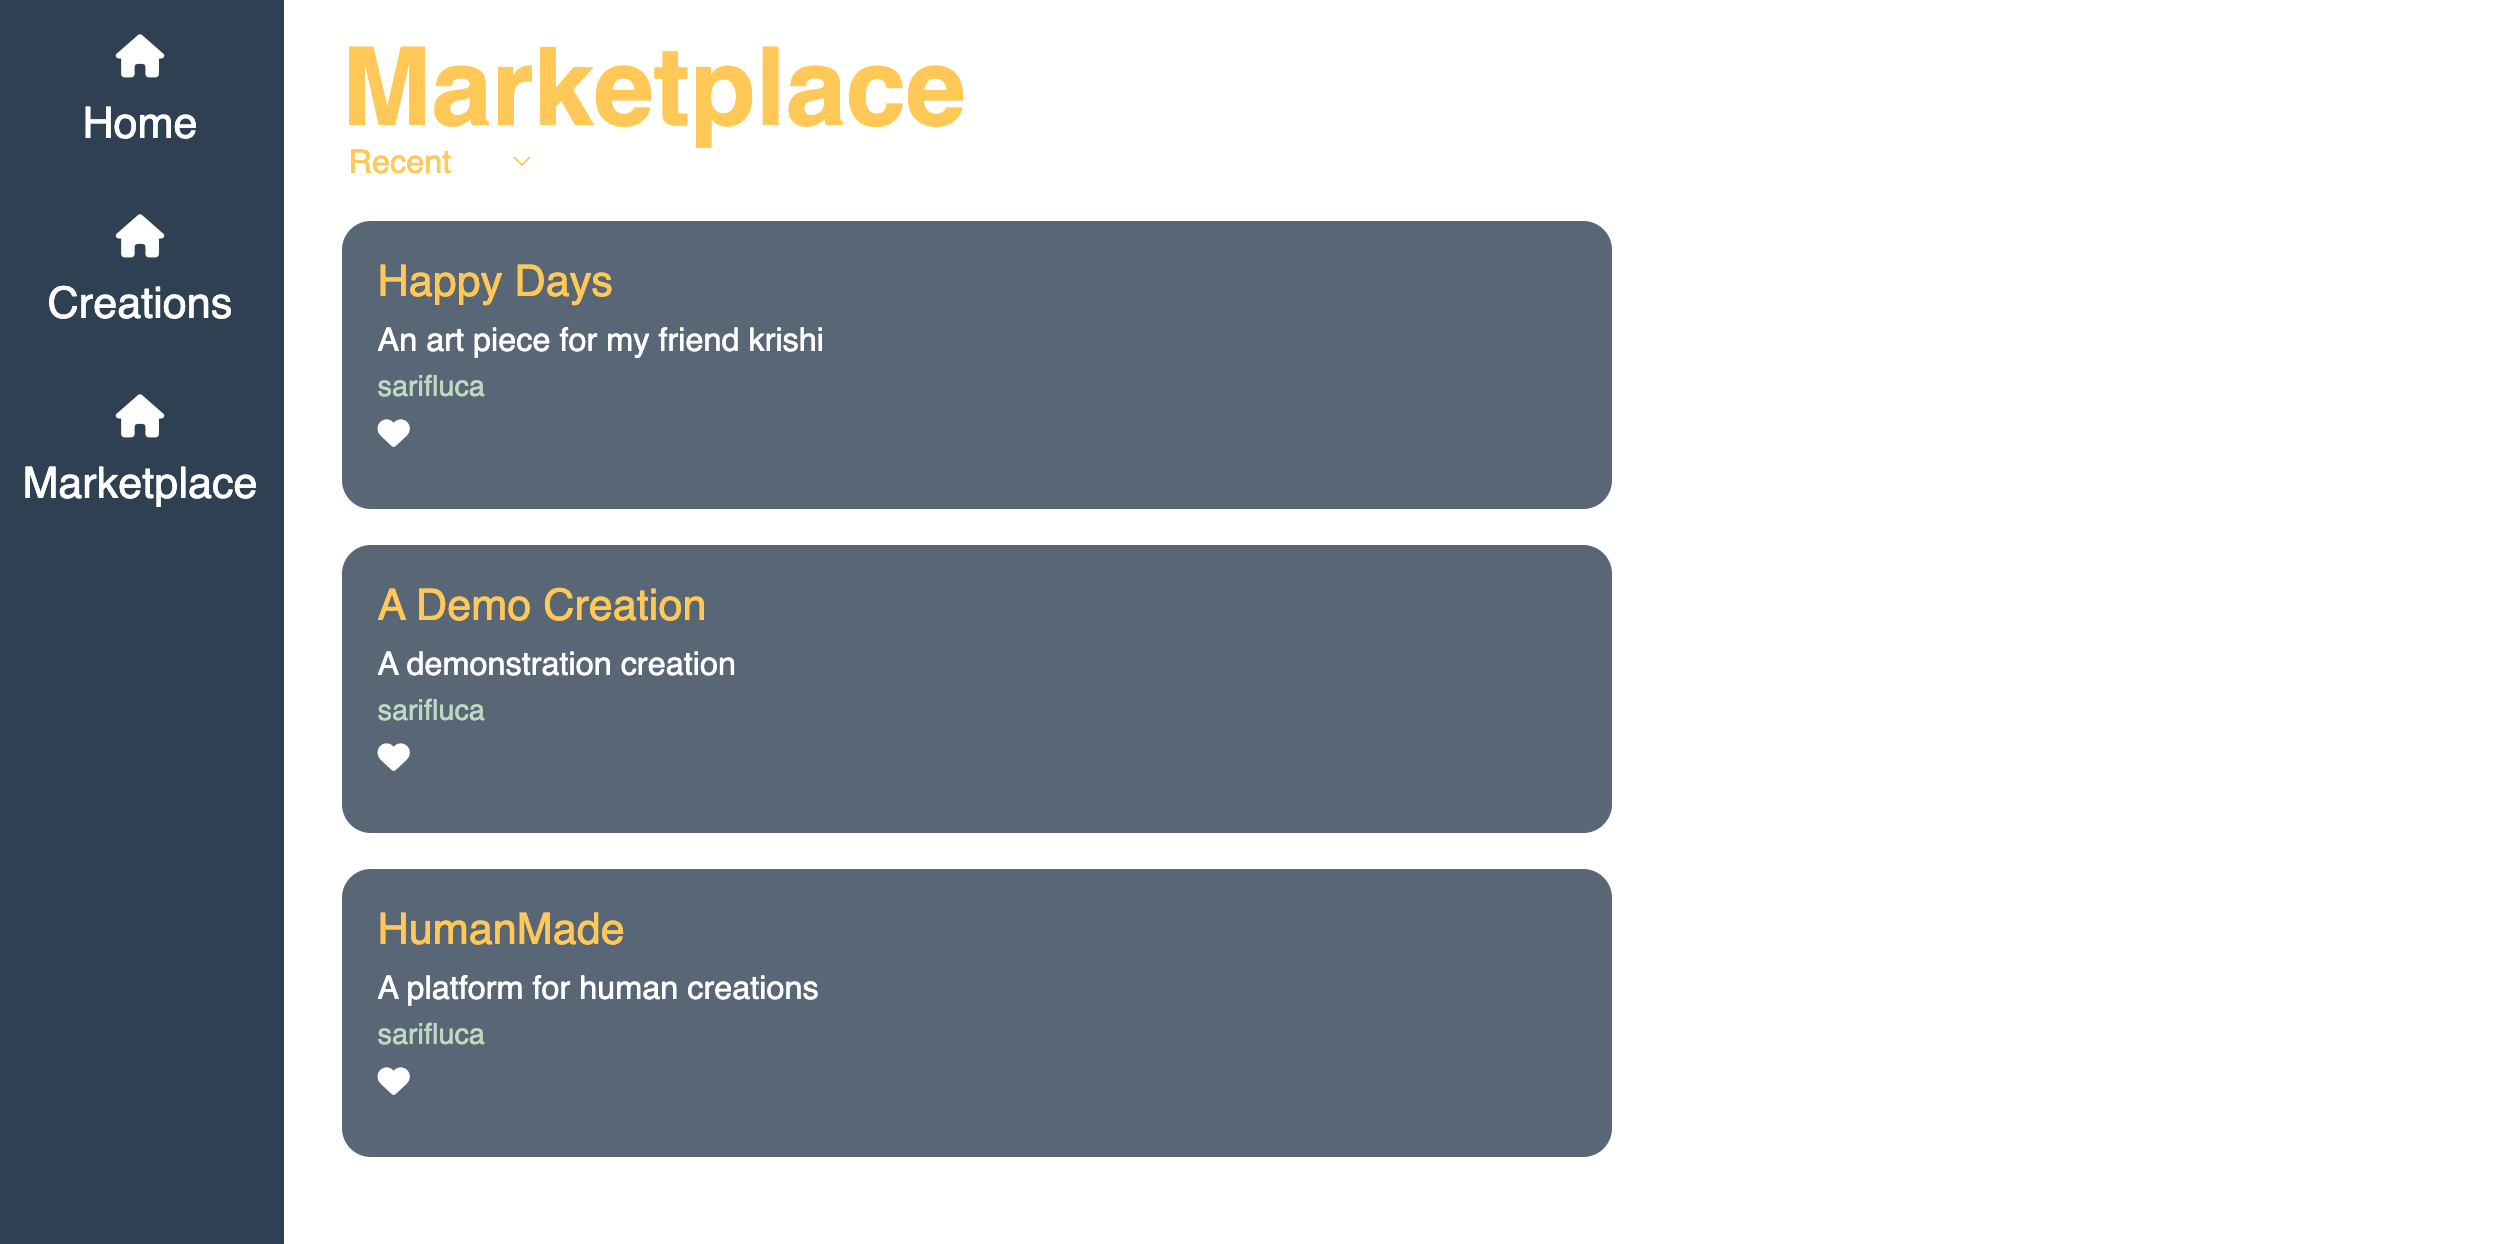
\includegraphics[scale=0.4]{marketplace.png}
\end{figure}
This allows consumers to view finished creations, including the progress timeline associated with it, from any creator. Consumers can also `like' marketplace creations by clicking the heart icon, which will turn yellow. Finished creations can be filtered by most recent or most liked, giving HumanMade it's community aspect.
\subsection{Blockchain Interface}
\begin{figure}[H]
    \centering
    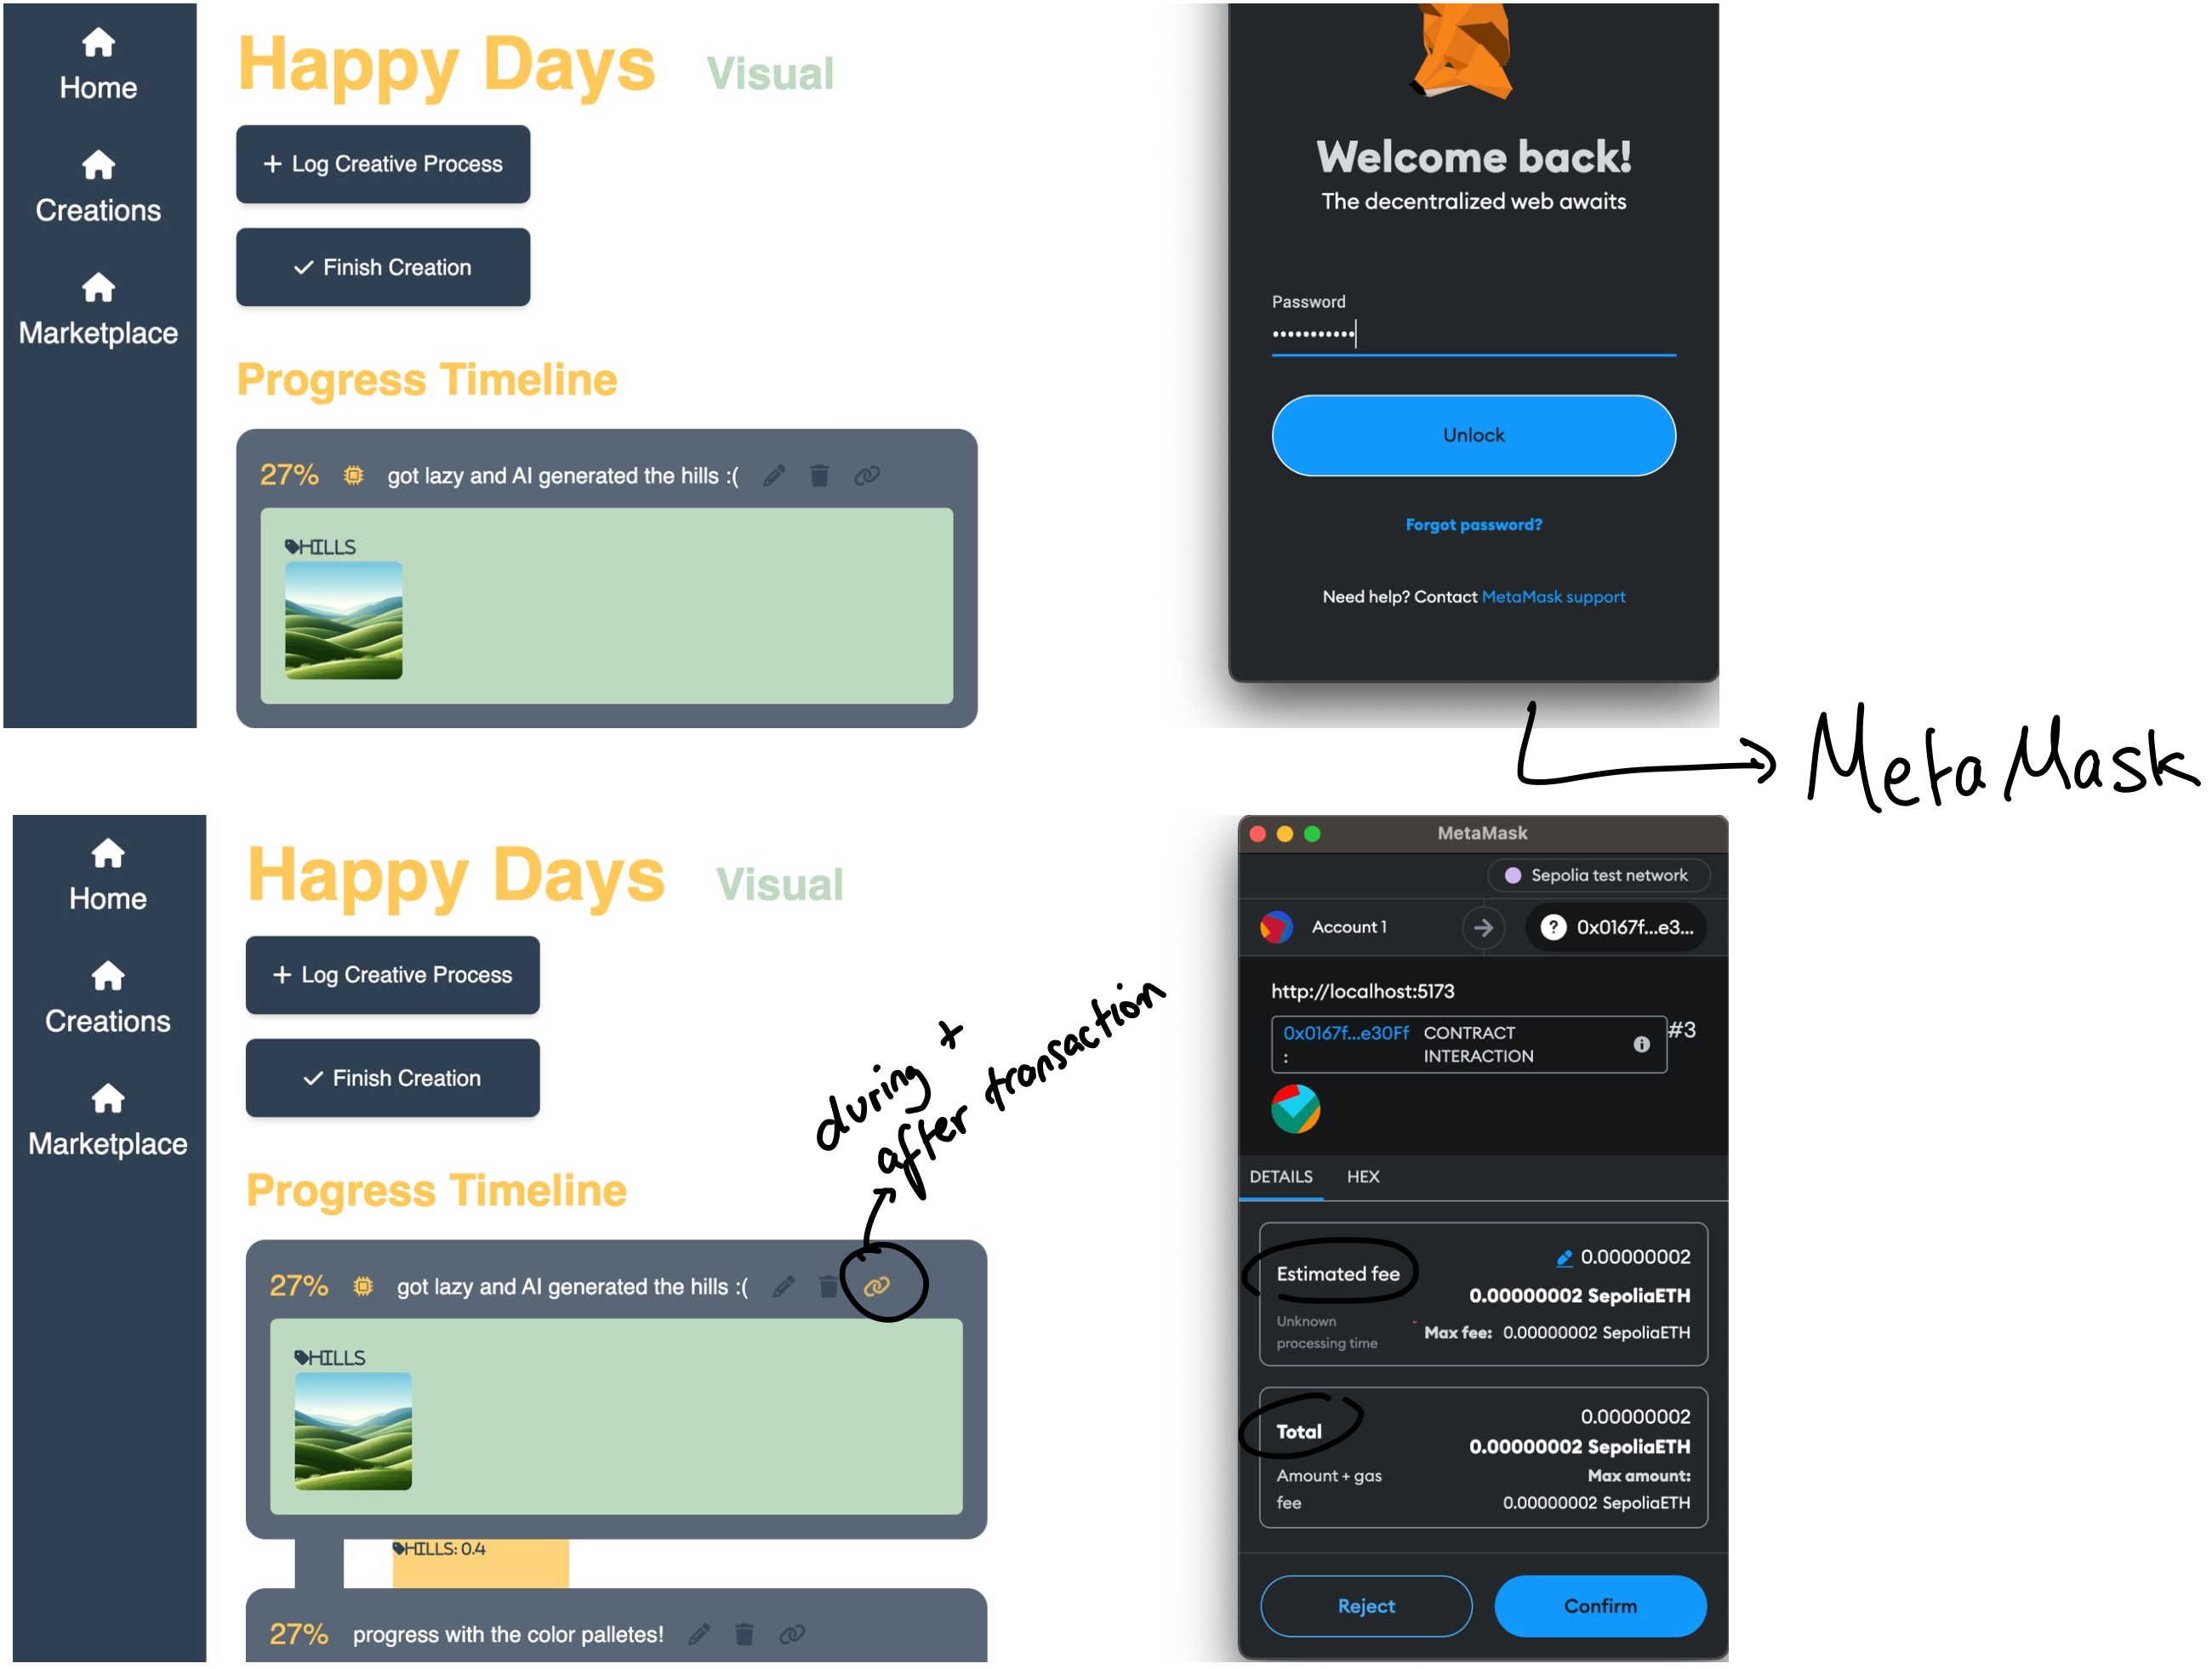
\includegraphics[scale=0.4]{metamask.png}
\end{figure}
When a user clicks on the link icon in the top right of any commit on the progress timeline, a MetaMask window will pop up. (If the user has not yet installed MetaMask, they will be prompted to do so). 
The user is then prompted to login to their wallet, and the details of the transaction are displayed. If the user chooses to confirm the transaction, the file data in the commit and the user's ID will be hashed together and recorded on the blockchain via a smart contract function. The link will then be highlighted yellow from then on if the transaction was successful.
\subsection{Command Line Interface}
The command line tool consists of 3 commands:
\begin{itemize}
    \item \textbf{login}, where the user specifies their email and later password in a hidden input
    \item \textbf{commit}, which takes arguments for the files, tags, description, percentage, and the creation ID to commit to
    \item \textbf{creations}, which lists all the creation ID's of the logged in user's creations.
\end{itemize}
The tool is written in Node.js and is run by using the \textbf{node} command, followed by the script path and required arguments.
\begin{lstlisting}
node dist/humanmade.js login --email="sarifluca@gmail.com"
node dist/humanmade.js creations
node dist/humanmade.js commit --files="me.jpg" --inputTags="me" --description="A photo of me" --usedAI=false --percentage=50 --creationID=HGbyrdJjJSjwxXoKh9wO
\end{lstlisting}
\section{Implementation}
\subsection{Architecture}
\begin{figure}[H]
    \centering
    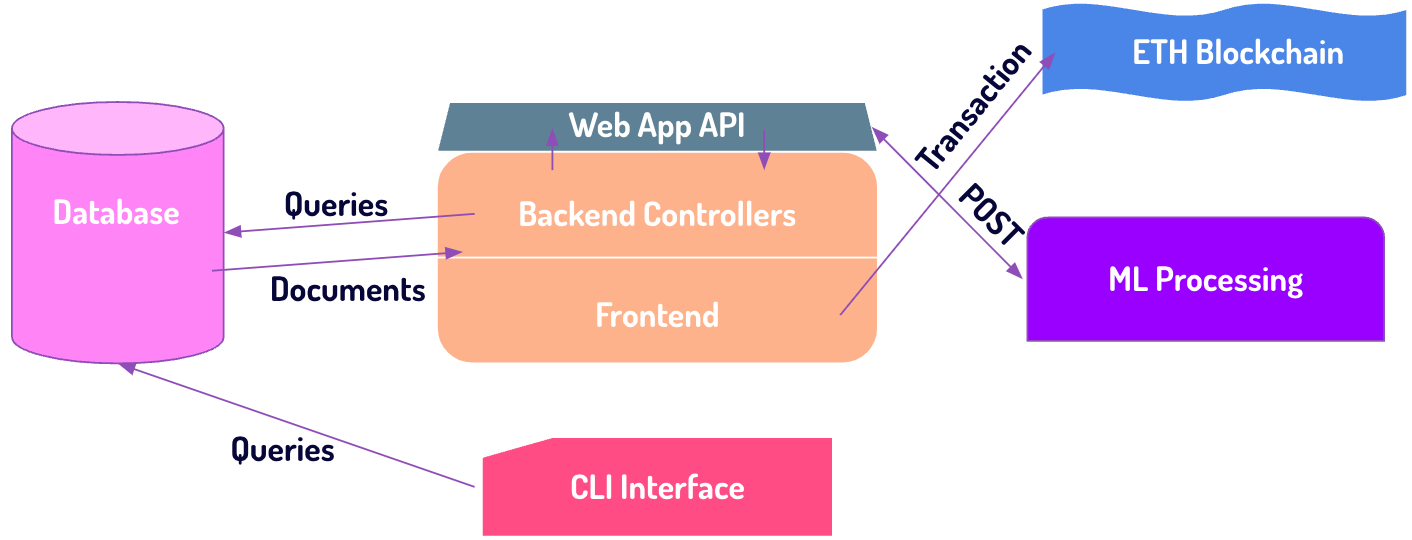
\includegraphics[scale=0.6]{architecture.png}
    \caption{System architecture for HumanMade. \cite{gpt4}}
\end{figure}
These components (apart from communication with the blockchain) all communicate via RESTful APIs, a simple and standardized format of communication between different services. REST APIs are stateless, facilitating scalability, flexibility and modularity of components. The client (web app) and any services it interacts with are decoupled and can be developed individually without dependencies. The Firebase SDK communicates via REST under the hood (in addition to web sockets for real-time data listening), keeping the architecture consistent and maintaining all the aforementioned benefits.
\subsection{Web App}
\subsubsection{Tech Stack}
After researching the many available web frameworks, middlewares and backend frameworks, I settled on a modern and scalable tech stack for the web app which would help me develop a reactive and robust app whilst writing clean code.
\begin{itemize}
    \item \textbf{SvelteKit} is a full-stack web framework which allows for a simple and modern approach to building fast, reactive web apps. SvelteKit features:
    \\\\
    Server-side rendering (SSR), allowing us to optimize the application for performance and search engine optimization (SEO). The server executes any JavaScript to generate the full HTML for the page, which is then sent to client. The benefit here is that the user sees a fully rendered page quickly, and search engines can crawl, index and in turn promote the content effectively. Then, hydration takes place; the server sends the JavaScript and application state, and event handlers are attached to the pre-rendered HTML, enabling interactivity with the website.
    \\\\
    Prefetching, where data for a page (and the page itself) is fetched when a user hovers the link for a page, pre-empting navigation and ensuring extremely fast load times. Prefetching is supported by the SvelteKit router out of the box.
    \\\\
    Filesystem-based routing, meaning the layout of files in the project dictates the route structure of the web app, simplifying setup and boilerplate code.
    \\\\
    Vite tooling under the hood, which provides fast build times with Hot Module Reloading (no need to refresh the page to see changes) and an optimized bundling process using Rollup. Tree shaking removes any unused code from the final build, and module bundling reduces the number of HTTP requests required to load the application.
    \\\\
    The ability to define API endpoints as server routes alongside other pages. This co-location makes it easier to manage frontend and backend code within a single project.
    \\\\
    In general, SvelteKit avoids common pitfalls found with traditional frameworks like React and Angular. These include large bundle sizes, the runtime overhead associated with a maintaining a shadow DOM, complex state management and SEO issues due to lack of SSR.
    \item \textbf{Tailwind} is an open source CSS framework. The UI is built by directly applying pre-defined styling classes to HTML elements. This allows for quick, consistent, and extensible styling, and works well with the component based methodology of SvelteKit. Tailwind has enamored developers for its customisability, configurability, and responsiveness, and has a strong community and ecosystem with plugins and UI kits. Tailwind also uses PurgeCSS, which removes unused CSS when building the web app for production, maintaining the light and fast load times already given to us by minified SvelteKit bundles.
    \item \textbf{Firebase} is a platform owned by Google offering a variety of tools and services to help developers build, improve and grow their apps. We will make use of the \textbf{Cloud Firestore} offering from Firebase as the primary database for the web app. 
    
    Firestore is a NoSQL database that allows for fast querying, dynamic data storage and automatic scalability. Security and analytics are built into the product, and there is a generous free tier to facilitate testing and initial deployment of the project. Firestore also has an excellent modular web SDK that will play well with a JavaScript frontend. 
    
    Additionally, Firebase offers \textbf{Cloud Storage}, a service for general blob storage of images, audio and video. This will be used for storing files associated with a commit. Again, security and scalability are integral. 
    
    Finally, Firebase offers an authentication service which allows for the easy creation and maintenance of user accounts with industry-leading security standards. JSON Web Tokens (JWTs) are used to manage sessions - these are secure, self-contained, and provide all the necessary information about a user. Firebase Authentication works seamlessly with Firestore to ensure users can only access information they are allowed to.
\end{itemize}

\subsubsection{General Structure}
Roughly, a SvelteKit project consists of:
\begin{itemize}
    \item a \verb|src/| directory. This contains all the application source code.
    \item \verb|src/routes| contains all the application's pages and endpoints. SvelteKit uses a filesystem-based routing system, so the folder \verb|src/routes/marketplace| will contain the code for the page route \verb|/marketplace|
    \item In each route folder, eg. \verb|src/routes/marketplace|, there is a \verb|+page.svelte|, \verb|+layout.svelte|, and potentially a \verb|+page.ts| or \verb|+page.server.ts|.\\\\ \verb|+page.svelte| contains the HTML and any frontend JavaScript for the webpage. \verb|+layout.svelte| contains HTML that can be used to apply a general layout to any pages in the same or nested folders. \\\\\verb|+page.ts| and \verb|+page.server.ts| are like the `backend' for a page, and contain load functions (eg. to load data from a database) which return data to the page upon initial loading, and form actions (functions which handle POST requests from a form element). There can also be a \verb|+layout.server.ts| which can contain a general load function which applies to any pages in the same or nested folders.
    \item \verb|src/lib| contains model code reused across the app. Components, utility functions, Svelte stores and type declarations all go here.
    \item \verb|src/routes/api| is where SvelteKit has you write any POST/GET API endpoints for your application. For example, adding a new folder named \verb|xyz|, containing a file named \verb|+server.ts| with a POST function, creates a new \verb|/xyz| endpoint on the web app that handles POST requests.
\end{itemize}
\subsubsection{UI/UX}
\textbf{Components:} SvelteKit is a component based web framework. Components are custom UI elements you create out of standard HTML elements. This allows for consistent styling, functionality and reusability across the app. Each component consists of:
\begin{itemize}
    \item a \verb|script| section containing exported component prompts and any interactive functionality
    \item the HTML for the component
\end{itemize}
For example, this excerpt from a \verb|Button.svelte| component consists of click, size, submit and icon props. 
\begin{lstlisting}
<script lang="ts">
    export let click = () => {};
    export let size = 'md';
    export let submit = true;
    export let icon = ''
</script>
\end{lstlisting}
and these props are passed to an HTML \verb|<button>| element
\begin{lstlisting}
<button 
    on:click={click}
    type={submit ? 'submit' : 'button'}
    ...
\end{lstlisting}
These props can be given values when the component is actually used in a parent webpage.
\begin{lstlisting}
<Button size="md" icon="fa-brush">Create</Button>
\end{lstlisting}
\textbf{Styling:} As aforementioned, instead of styling directly with CSS, I used the more modern approach of going with a CSS framework, specifically Tailwind. Tailwind consists of many modular, pre-defined utility classes which let you style elements rapidly and inside the HTML. This div is styled to be a flexbox, with a specified width and rounded corners.
\begin{lstlisting}
<div class="flex flex-col gap-2 w-6/12 rounded-2xl bg-opacity-80 bg-primary p-5">
\end{lstlisting}
For example, the \verb|flex| class is defined by Tailwind as:
\begin{lstlisting}
.flex {
    display: flex;
}
\end{lstlisting}
Notice the background is set to be \verb|bg-primary|. Thanks to Tailwind's configurability, we can specify a color palette, font family and font sizes in a \verb|tailwind.config.js|, and Tailwind will automatically incorporate our choices into the generated CSS class options.
\begin{lstlisting}
colors:{
    'primary': '#2E4052',
    'secondary': '#FFC857',
    'tertiary': '#BDD9BF',
    'quaternary': '#412234'
},
\end{lstlisting}
\textbf{Icons:} Iconography is important for aesthetics and accessibility. Font Awesome is a library that provides high-quality minimalist SVG icons for websites. It exposes these assets via CSS classes, meaning just as with Tailwind we can reference icons directly in the markup of our website, providing consistency and cleanliness across the codebase. 
\subsubsection{Authentication}
Firebase has simple API methods for creating and authenticating users with an email and password combination. The authentication flow is as follows:
\begin{enumerate}
    \item In the event that either method is successful, a result object is returned with a user property containing the user ID, display name and email.
    \item We extract and save these into a custom User type object, (and write a user document to the Firestore database if this is a new user), and then set a `user' cookie value to this object (serialised).
    \item We then have a \verb|+layout.server.ts| at the root of \verb|src/routes| containing a load function which returns the user object from the cookie.
    \item  This load function applies to all webpages, safely and efficiently exposing the user object to all pages which require it.
\end{enumerate}
Using Firebase authentication with Firestore makes the app seamlessly secure. We can write custom security rules in Firestore to restrict user access to certain documents in the database. For example, here we ensure that a creation can only be edited by the original owner of the creation:
\begin{lstlisting}
match /creations/{document=**} {
  allow write: if request.auth.uid == resource.data.uid;
}
\end{lstlisting}
Firebase authentication handles attaching the JWT to any database requests the user makes, giving Firestore access to the \verb|request.auth| object to use in security rules.
\subsubsection{Reactivity \& Updates}
To ensure a reactive and responsive experience for users, we develop a way to keep the client and server in sync with a clean and elegant approach.
We take advantage of Svelte reactive stores and Firestore realtime listeners.\\\\
\textbf{Svelte Stores:} These are helpful for managing global state across components. The type of store we use is \verb|writable|, where we store arrays either of type \verb|Creation| or \verb|Product|, for the creation and marketplace tabs respectively. We can read and write values to these arrays, via the \verb|update| and \verb|set| methods of the store, and more importantly we can now subscribe to the store. Then, any components relying on the store values are automatically re-rendered by SvelteKit upon updates to the store. For example, this \verb|each| loop will re-render any of the necessary \verb|CreationDiv| components upon any updates to the \verb|creations| store.
\begin{lstlisting}
{#each $creations as creation (creation.id)}
    <CreationDiv {creation}></CreationDiv>
{/each}
\end{lstlisting}
\textbf{Realtime Listeners:} These simply subscribe to a collection of documents in the Firestore database, triggering upon any changes to the collection. Firebase returns a collection of \verb|DocumentChange|s, which supplies the document which was updated and the type of update (added, modified or removed).
\\\\
Using these two concepts, we can map changes we see from the listener to changes in the store, allowing us to efficiently update UI every time the database state changes. To do this mapping cleanly, we implement a \verb|Listener| wrapper class for each store, which gives us methods to easily update the store from listener document updates. 
\begin{lstlisting}
abstract class Listener<T>{
    abstract update(struct: T): void;
    abstract remove(struct: T): void;
    abstract add(struct: T): void;
    abstract docToType(doc: DocumentSnapshot): T;
}
\end{lstlisting}
\noindent
The diagram below illustrates the approach at a high level.
\begin{figure}[H]
    \centering
    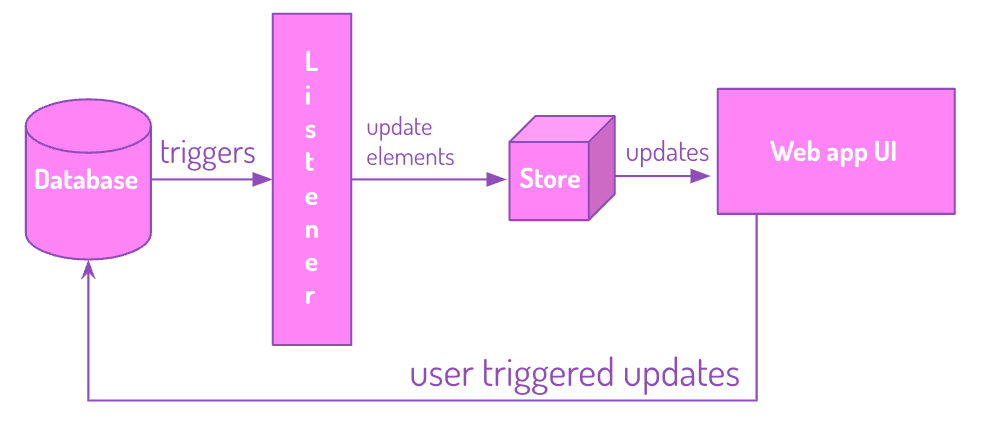
\includegraphics[scale=0.8]{reactivity.png}
    \caption{Reactivity system for HumanMade\cite{gpt4}}
\end{figure}
\noindent For `user triggered updates', we use the `addDoc', `updateDoc' and `deleteDoc' Firestore SDK methods, which are fairly trivial to use. These take the collection we want to edit, the document title, and document details if relevant. 
\noindent By doing this, the entire web app is fully responsive and reactive, meaning a user never needs to refresh the page to see changes or the latest database state. Everything from editing a commit description to viewing a new creation on the marketplace is done in real-time and synced up automatically. No jittery or slow loading animations.
\subsubsection{Accessibility}
To ensure accessibility, we followed WCAG requirements closely. These are organised into four main principles to follow:
\begin{enumerate}
    \item Perceivable: Information and user interface components must be presented in ways that users can perceive. We make sure to include text, icons and color changes upon hovering for all interactive buttons and components, clearly and intuitively signifying to a user of any background their purpose and functionality.
    \item Operable: User interface components and navigation must be operable. The interface cannot require interaction that a user cannot perform. Using Playwright tests, detailed later on, we ensure this is the case for all pages of the application.
    \item Understandable: Information and the operation of the user interface must be understandable. Users must be able to understand both the information and the operation of the user interface.
\end{enumerate}



Robust: Content must be robust enough that it can be interpreted reliably by a wide variety of user agents, including assistive technologies. This means that users must be able to access the content as technologies advance.
\subsection{Machine Learning Microservice}
\subsubsection{Tech Stack}
\begin{enumerate}
    \item \textbf{TensorFlow} is a free and open-source machine learning library from Google, providing state of the art models and APIs in Python. Consequently this was a straightforward choice to make.
    \item \textbf{Flask} is a micro web framework written in Python, perfect for setting up a simple API for the microservice with which the main web app can interoperate. 
\end{enumerate}
This microservice handles computation of the similarity score between images of the same tag across commits, as described in the functionality section.
\subsubsection{Firebase Storage} Any images uploaded in a commit are stored in cloud storage, with a \verb|+| separated filename consisting of the image \verb|tag|, \verb|file.type| and the current date to avoid the chance of duplicate filenames.
\subsubsection{Data Flow} The data flow when interacting with the ML processing microservice is as follows, and is also detailed in the below diagram.
\begin{figure}[H]
    \centering
    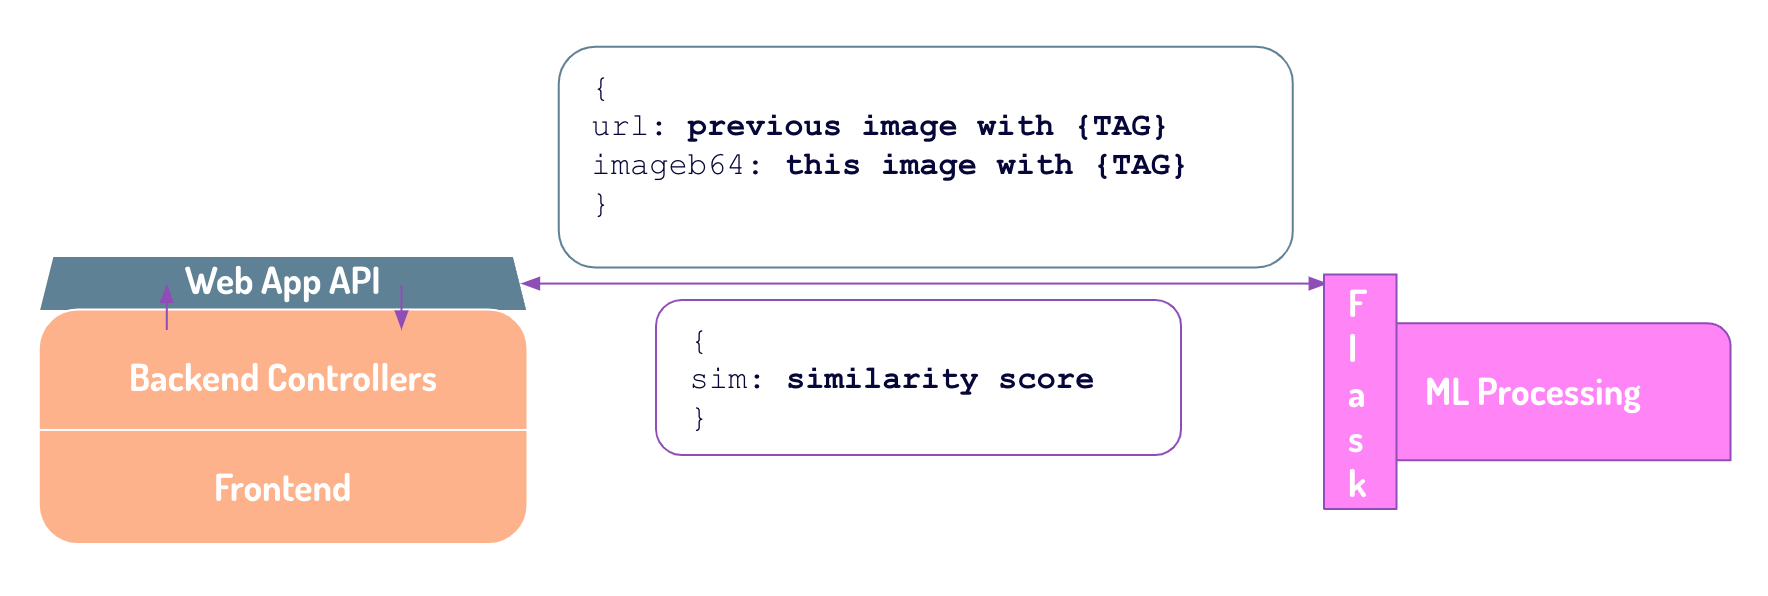
\includegraphics[scale=0.6]{ml.png}
    \caption{Data flow diagram for the ML microservice}
\end{figure}
Upon a new commit to the progress timeline containing an image tagged \verb|{tag}|, and given there is an image with tag \verb|{tag}| in the previous commit:
\begin{enumerate}
    \item The base 64 encoding of the image in the current commit, and the URL (provided by Firebase Storage) of the image in the previous commit are posted in JSON to the \verb|/imageSimilarity| API endpoint. 
    \item The microservice processes the images (detailed in the next section), and returns back a similarity score to the web app API's request.
    \item The web app endpoint returns the similarity score to the frontend, and this is displayed on the progress timeline if below a certain threshold.
\end{enumerate}
\subsubsection{Similarity Computation} ResNet50, a 50 layer Convolutional Neural Network provided by the Tensorflow library, is used to extract a high level feature vector from each of the images. These two vectors are then compared using cosine similarity.\\

Firstly, we preprocess the images:
\begin{itemize}
    \item Images are received by Flask in a POST method. The images are downloaded and written to \verb|.jpg| files. 
    \item Images are size adjusted (ResNet required images to be in \verb|224x224| resolution) and converted to a 3D array (width by height by color channels, (224,224,3)). ResNet actually takes input in 4D, where the first dimension represents batch size, so we need to expand our array to dimensions (1,224,224,3).
    \item Finally, the TensorFlow-provided \verb|preprocess_input()| function scales and normalises pixel values of the image.
\end{itemize}
Then, we can extract a feature vector for each image: ResNet50 is a classification model, with its final layer consisting of 1,000 different classes. We do not want to classify our images - so, we stop the model at an intermediate layer, giving us a high level feature vector describing the images. We can do this with the provided \verb|Model| python class, which lets us specify a base model and a specific layer to be our output. ResNet50 consists of pooling, convolutional and ReLU activation layers. 

We choose a late convolutional layer to stop at. We specify a convolutional layer, as these are where kernels/filters are applied to the image to better detect high level abstract features \cite{convNN}, and we specify a late layer, since as we move further into the network more information on patterns and high-level features of the image are encoded into the feature vector. Both of these properties are what we desire when comparing similarity in our case. The general shape, color and vibe of an image should not change drastically commit to commit as a user is working on a project, whereas specific pixel values and details could and should be allowed to vary.
\begin{figure}[H]
    \centering
    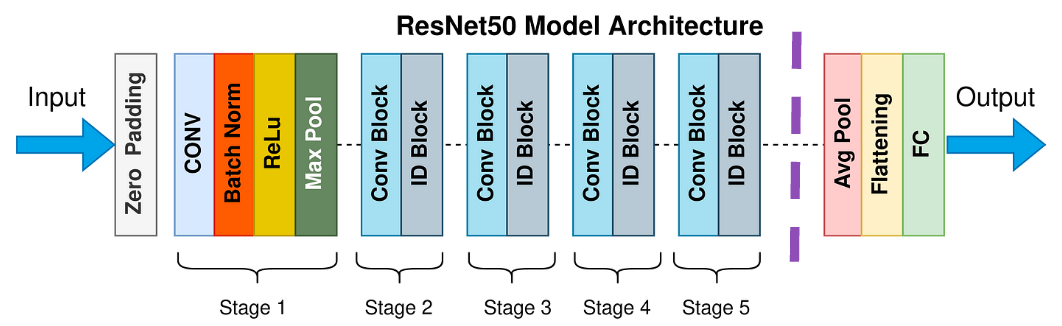
\includegraphics[scale=0.8]{resnet.png}
    \caption{We look to cut off ResNet's output early, represented by the purple dashed line.}
\end{figure}
Finally, we use cosine similarity (\verb|1-cosine(vec1, vec2)|) to compare the feature vectors. At a high level we can think of this as measuring the `direction' of the vectors in \verb|n|-dimensional space and seeing how closely they align.
\begin{figure}[H]
    \centering
    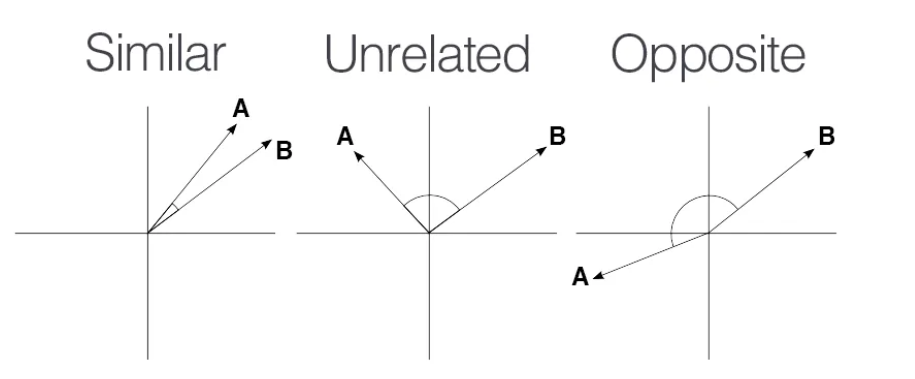
\includegraphics[scale=0.5]{cosine.png}
    \caption{A diagram representing cosine similarity.}
\end{figure}

\subsection{Blockchain Interface}
\subsubsection{Tech Stack}
\begin{itemize}
    \item \textbf{MetaMask} is the leading self-custodial cryptocurrency wallet, also used to interact with the Ethereum blockchain (known as a provider). Users can access their wallet and perform transactions with ease, without having to send their private key across a network thanks to the MetaMask Browser extensions that integrates tightly with web apps.
    \item \textbf{Solidity} was an obvious choice, being the defacto programming language for implementing smart contracts on the Ethereum blockchain. It has a strong ecosystem, robust development tools (like Web3.js and Remix) and enhanced security features.
    \item \textbf{Remix} is an open-source IDE widely used for Ethereum smart contract development. We use Remix to compile, deploy and test our smart contract. 
    
    Remix is optimized for Solidity, providing syntax highlighting, code completion, and other features to streamline the developer experience. Remix also provides various alternative options for deployment of the contract, including test-nets and virtual blockchains, which are important during development.
    \item \textbf{Web3.js} is a collection of open-source libraries that primarily provides an abstracted interface for communication with an Ethereum provider, as well as other helpful utility functions. This is the immediate layer we use to interface with the Blockchain from our frontend JavaScript, and also helps us create our transaction object. 
    
    Web3.js is widely adopted, with robust support and extensive documentation. Crucially, it works seamlessly with MetaMask acting as a provider, giving tight and clean integration for a cutting-edge end-to-end user experience.
\end{itemize}
\subsubsection{Smart Contract Development}
A smart contract can be thought of as a self-executing contract whose methods a user can interact with by sending crypto to.

For the purposes of HumanMade, we want to use the automated execution aspect of smart contracts, along with the immutable and secure aspects of the blockchain itself. We will use a smart contract function to record information about a commit on the chain, requiring the user to send no crypto to complete the transaction.
\\\\
The code for the smart contract we are using is fairly short, consisting of a 
\\\verb|makeCommit(string[] fileHashes)| function, which emits an event\\ \verb|CommitMade(msg.sender, hash)| that could be used to trigger actions in other decentralized applications in the future. For the purpose of this application, the \verb|makeCommit| function is of importance, as the value passed into this is what gets recorded in a transaction on the blockchain when invoked.\\\\
We then use Remix to compile and deploy the contract. The Solidity contract is compiled down to bytecode, and can then be deployed to either:
\begin{enumerate}
    \item the Ethereum main-net
    \item an Ethereum test-net
    \item a virtual JavaScript network in the browser
\end{enumerate}
We opt for option 2, deploying the contract to the Sepolia test-net, a proof-of-stake network designed to mimic the operating environment of the main-net but existing on a separate blockchain ledger. This allows us to test our smart contract without risking real value. We can receive free Sepolia ETH tokens to use on this test-net via many of the available Sepolia `faucets'.

This is in fact the only viable option. At least until it is required in production, we don't want to have to pay the (sometimes exorbitant) gas fees required to commit a contract (or conclude any transaction) to the main-net during testing, which option 1 would require. We also want to be able to test our contract in as close to a real-world scenario as possible, using an actual transaction signed with MetaMask, which would not be possible if we deployed our contract to a virtual browser network with option 3.

Deploying via Remix to the Sepolia testnet, (paying the gas fees required to do this using a wallet with Sepolia ETH in it), gives us the contract address and contract Application Binary Interface (ABI), which is all the information we need to make a transaction with the contract. The ABI simply represents the contract in a structured format, allowing calls to the contract to be encoded into bytecode which the Ethereum Virtual Machine can execute.
\begin{figure}[H]
    \centering
    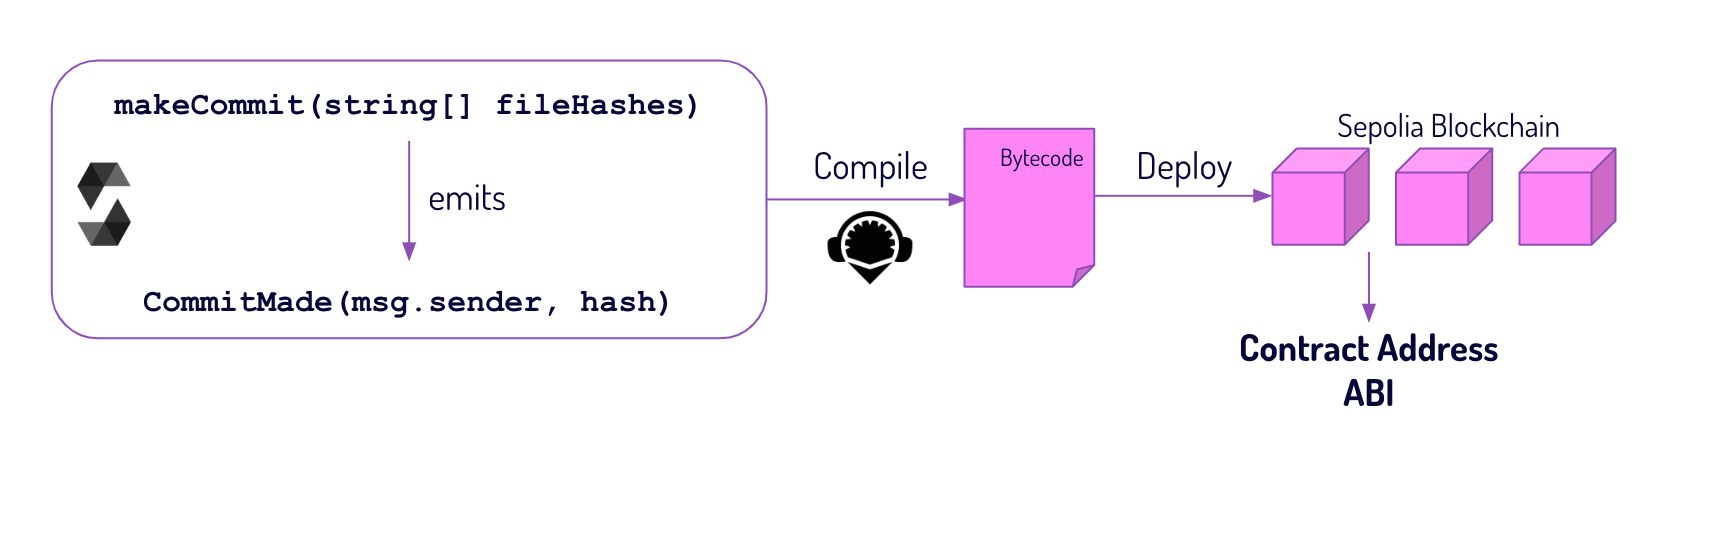
\includegraphics[scale=0.6]{deploy.png}
    \caption{The process for compiling and deploying the Solidity smart contract}
\end{figure}
\subsubsection{Communication Setup}
To communicate with the blockchain using the Web3.js interface, we need to pass the \verb|Web3| constructor a `provider'.
A provider is an object which facilitates communication with an Ethereum node, supplying essential properties and methods which adhere to the Ethereum Provider API standard. MetaMask supplies us with this object when installed, injecting a \verb|window.ethereum| object into the browser for web apps to make use of.
\begin{lstlisting}
const web3 = new Web3(window.ethereum);
\end{lstlisting}
Now that \verb|Web3| is invoked with a valid provider, we can create a Contract object which will let us execute our contract methods on the chain. This is where we need the contract address and ABI:
\begin{lstlisting}
const contract = 
    new web3.eth.Contract(JSON.parse(abi), address);
\end{lstlisting}
Now, we have access to all the methods we need to perform a transaction on the chain.
\subsubsection{Performing Transactions}
We want the transaction we perform to contain content related to the files in the progress timeline commit, and to the user themselves. So, we hash each file in the commit with the user ID, and pass an array of hashes into our contract method. This way, each commit is tamper-proof and traceable, with the original content and creator recorded permanently on the blockchain ledger.
Upon a user clicking the `link' icon on a progress timeline commit:
\begin{enumerate}
    \item We get the contract address and ABI. These are stored on the server for safety, so the backend controller makes a call to a \verb|/blockchainCommit| API endpoint to get these details first. 
    \item We request access to the MetaMask account, obtaining the user's wallet address.
    \item We create the transaction object - a simple JavaScript object where we pass:
    \begin{itemize}
        \item the receiver, in this case the contract address
        \item the sender, in this case the user's wallet
        \item a data string the Ethereum Virtual Machine can interpret as a command, in this case a string of bytecode representing a call to the contract method \verb|makeCommit|. We can obtain this using the Contract object we created earlier in the setup phase.
        \begin{lstlisting}
data: contract.methods.makeCommit(commit.hashes).encodeABI()
        \end{lstlisting}
        \item the user's transaction count (the nonce, which provides a unique ID for each transaction and ensures transactions are ordered and executed correctly)
        \item gas fees and the gas limit. We calculate the fee based on the gas fee of the latest block which has been added to the chain, and the limit based on the size of the transaction object.
    \end{itemize}
    \item We make a transaction call using the Web3.js object we invoked:
    \begin{lstlisting}
const txHash = await web3.eth.sendTransaction(txObject);
        \end{lstlisting}
        and this in turn sends the transaction object in the form of a JSON-RPC message to MetaMask. 
    \item MetaMask can then sign the transaction object with the user's private key, and forward the message to an Ethereum node for us. Ethereum nodes act as a point of access to the blockchain, enabling interactions like sending transactions. Developers can interact with some nodes remotely via JSON-RPC APIs, such as those run by software company Infura.
    \item Upon receiving the JSON-RPC, the node will parse the request, ensure the transaction is valid (sender's key signature, ensuring the sender has enough ETH for gas fees, confirming nonce etc.), and then execute the bytecode command found in the \verb|data| property on the Ethereum Virtual Machine.
    \item The smart contract function is run, and the transaction will be included in the next block on the chain.
\end{enumerate}
\begin{figure}[H]
    \centering
    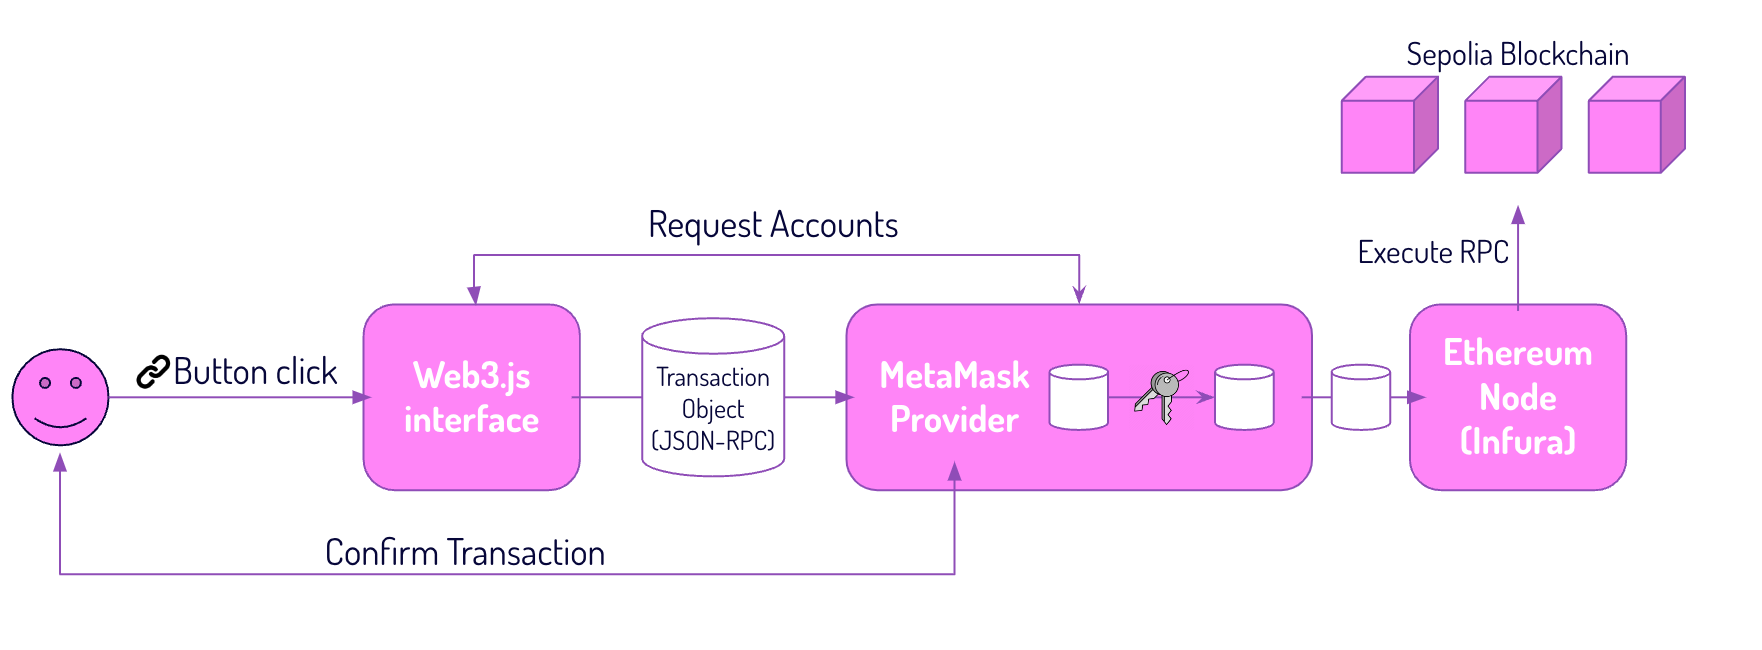
\includegraphics[scale=0.6]{bchain.png}
    \caption{The full process of performing a transaction end-to-end}
\end{figure}
Finally, we save the transaction hash we receive back to the database, letting the main application identify that the commit has been recorded on the blockchain.
\subsection{Command Line Interface}
\subsubsection{Tools Used}
\begin{itemize}
    \item \textbf{Node.js} is the defacto language and runtime for out-of-browser JavaScript. It allows us to write our command line tool in Typescript, make network requests and take advantage of the flourishing library ecosystem.
    \item \textbf{Yargs} is a popular library for building command line tools in Node.js, providing an easy and abstracted way to specify commands and their functionality.
    \item \textbf{Inquirer} is a popular library for building command line interface prompts.
\end{itemize}
\subsubsection{Authentication}
The user needs to be able to authenticate directly with Firebase through the command line interface, in order to securely commit to a creation.
\begin{itemize}
    \item The user will specify their email when using the login command.
    \item Once executed, the command will prompt the user for their password, using Inquirer to ensure the input is hidden.
    \item We can then use the same Firebase authentication methods provided for node as we did in the web app, giving us a \verb|result| object in return.
    \item The difference now is we need to manually handle storing the authentication token for the user. We can extract the JSON Web Token (JWT) used to identify the user to a Firebase service from the \verb|result| object, and cache this in a text file. 
    \begin{lstlisting}
let token = await res.user.getIdToken();
await fs.promises.writeFile("./HumanMade/token.txt", token);
    \end{lstlisting}
    The user can then use the command line tool freely until the token expires, in which case they would use the \verb|login| command again. 
\end{itemize}
The Firebase SDK which would normally sign the requests for a user automatically, as in the web app, only works within a browser environment. We must instead use the Firebase REST API in conjunction with the JWT.
\subsubsection{Firebase REST API}
We use the fetch API to interact with Firebase via the REST API. The base URL for all requests we will make is of the following form:
\begin{lstlisting}
const baseUrl = https://firestore.googleapis.com/v1/projects/${projectId}/databases/(default)/documents
\end{lstlisting}
In every (POST) request to the API, we send the JWT along in the \verb|Authorization| property of the header. This lets Firebase Firestore identify the user querying the database, ensuring database requests adhere to security rules.
\\\\
If we want to query data, as in the case of querying creation IDs with the \textbf{creations} command, we can post a \verb|StructuredQuery| JSON object to the \verb|`${baseUrl}:runQuery`| endpoint. A \verb|StructuredQuery| object can specify all the attributes we would normally use when querying using the Firebase SDK, including \verb|where| clauses and a \verb|from| property to specify which collection we would like to query from. 
\\\\
Creating data, as in the case of creating a new commit with the \textbf{commit} command, we similarly POST a JSON object specifying the fields of the document we want to create, along with the JWT in the header. In the process of creating a commit we also handle image similarity across any images with the same tag, querying the \verb|/imageSimilarity| microservice endpoint.
\section{Testing, Performance \& Deployment}
TODO DEPLOYMENT
\subsection{Playwright}
Playwright is an open source automation library for end-to-end browser testing, providing the ability to automate browser tasks in Chromium, Firefox and WebKit with a single API. We use playwright to test the robustness and correctness of the application.

A Playwright test is wrapped in the \verb|test| API function, and the general structure is as follows:
\begin{enumerate}
    \item We start by navigating to the page we want to test:
    \begin{lstlisting}
    await page.goto('https://localhost:5173/creations');
    \end{lstlisting}
    \item We then simulate user interactions such as clicking buttons or entering text. We can select elements by ID by using a hash:
    \begin{lstlisting}
        await page.click('button#addNew');
        await page.fill('input#name', 'Test Creation');
        await page.click('button#submit');
    \end{lstlisting}
    \item Finally, we assert that the web app responded correctly to the simulated user input:
    \begin{lstlisting}
        await expect(page).toHaveText('Test Creation');
        await expect(page.locator('input#name')).toBeEmpty();
        await expect(page).toHaveURL('/creations');
    \end{lstlisting}
\end{enumerate}
Upon running the tests with the Playwright NPM package, we are alerted of any assertions which are violated and can ensure our application runs as intended throughout the development process. Playwright also assists in taking advantage of Test Driven Development (TDD), which is where we write the test for a web page yet to be developed, giving us a clear outline and goal of the functionality and purpose of the page. This helped greatly with speeding up the development process and ensuring the correct and relevant functionality was being implemented at all times.
\subsection{Postman}
Postman lets us test the numerous interactions we have involving REST APIs across our application, providing a comprehensive UI which lets us specify an endpoint URL, parameters, the body of the request and the HTTP action type. We can then view the response (along with status and time) in pretty-ified JSON, making testing and development of the services we interact with through APIs much easier. 
\begin{figure}[H]
    \centering
    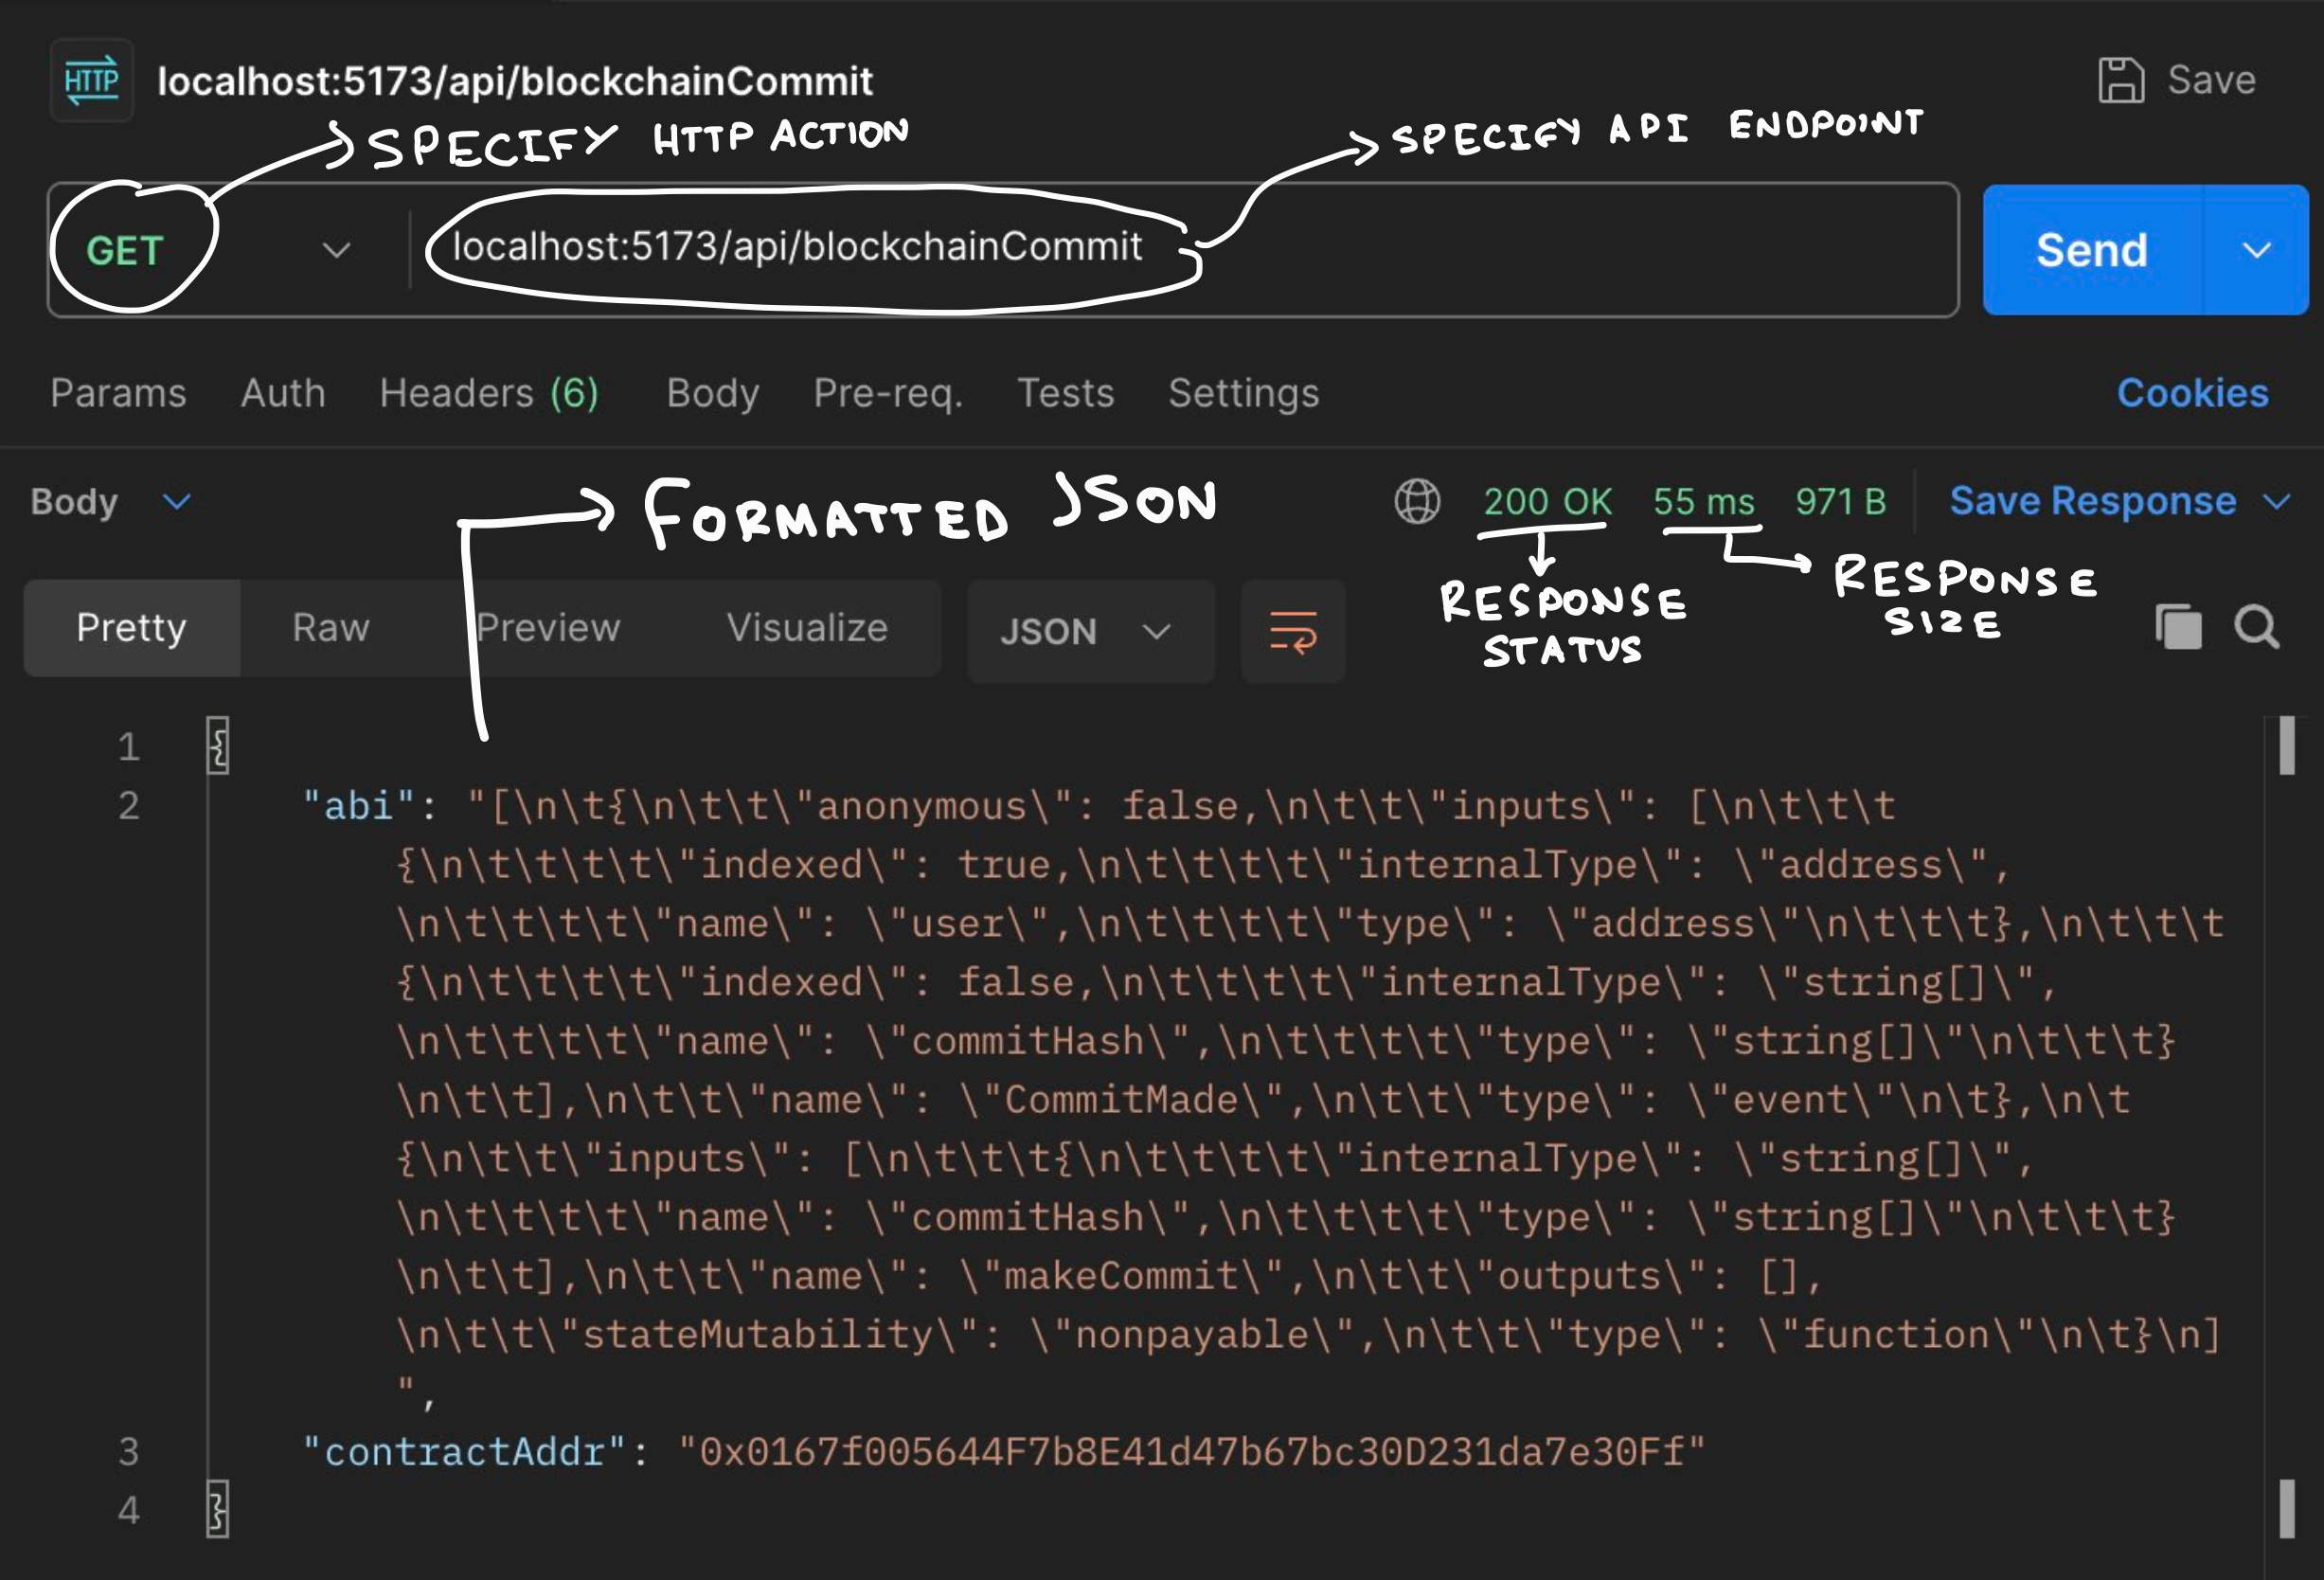
\includegraphics[scale=0.4]{postman1.png}
    \caption{The full process of performing a transaction end-to-end}
\end{figure}
\noindent For example, here we test the \verb|/blockchainCommit| API endpoint belonging to our web app. This is a fairly simple GET request, whose response we check contains the correct contract details we expect back for performing the blockchain transaction.

\begin{figure}[H]
    \centering
    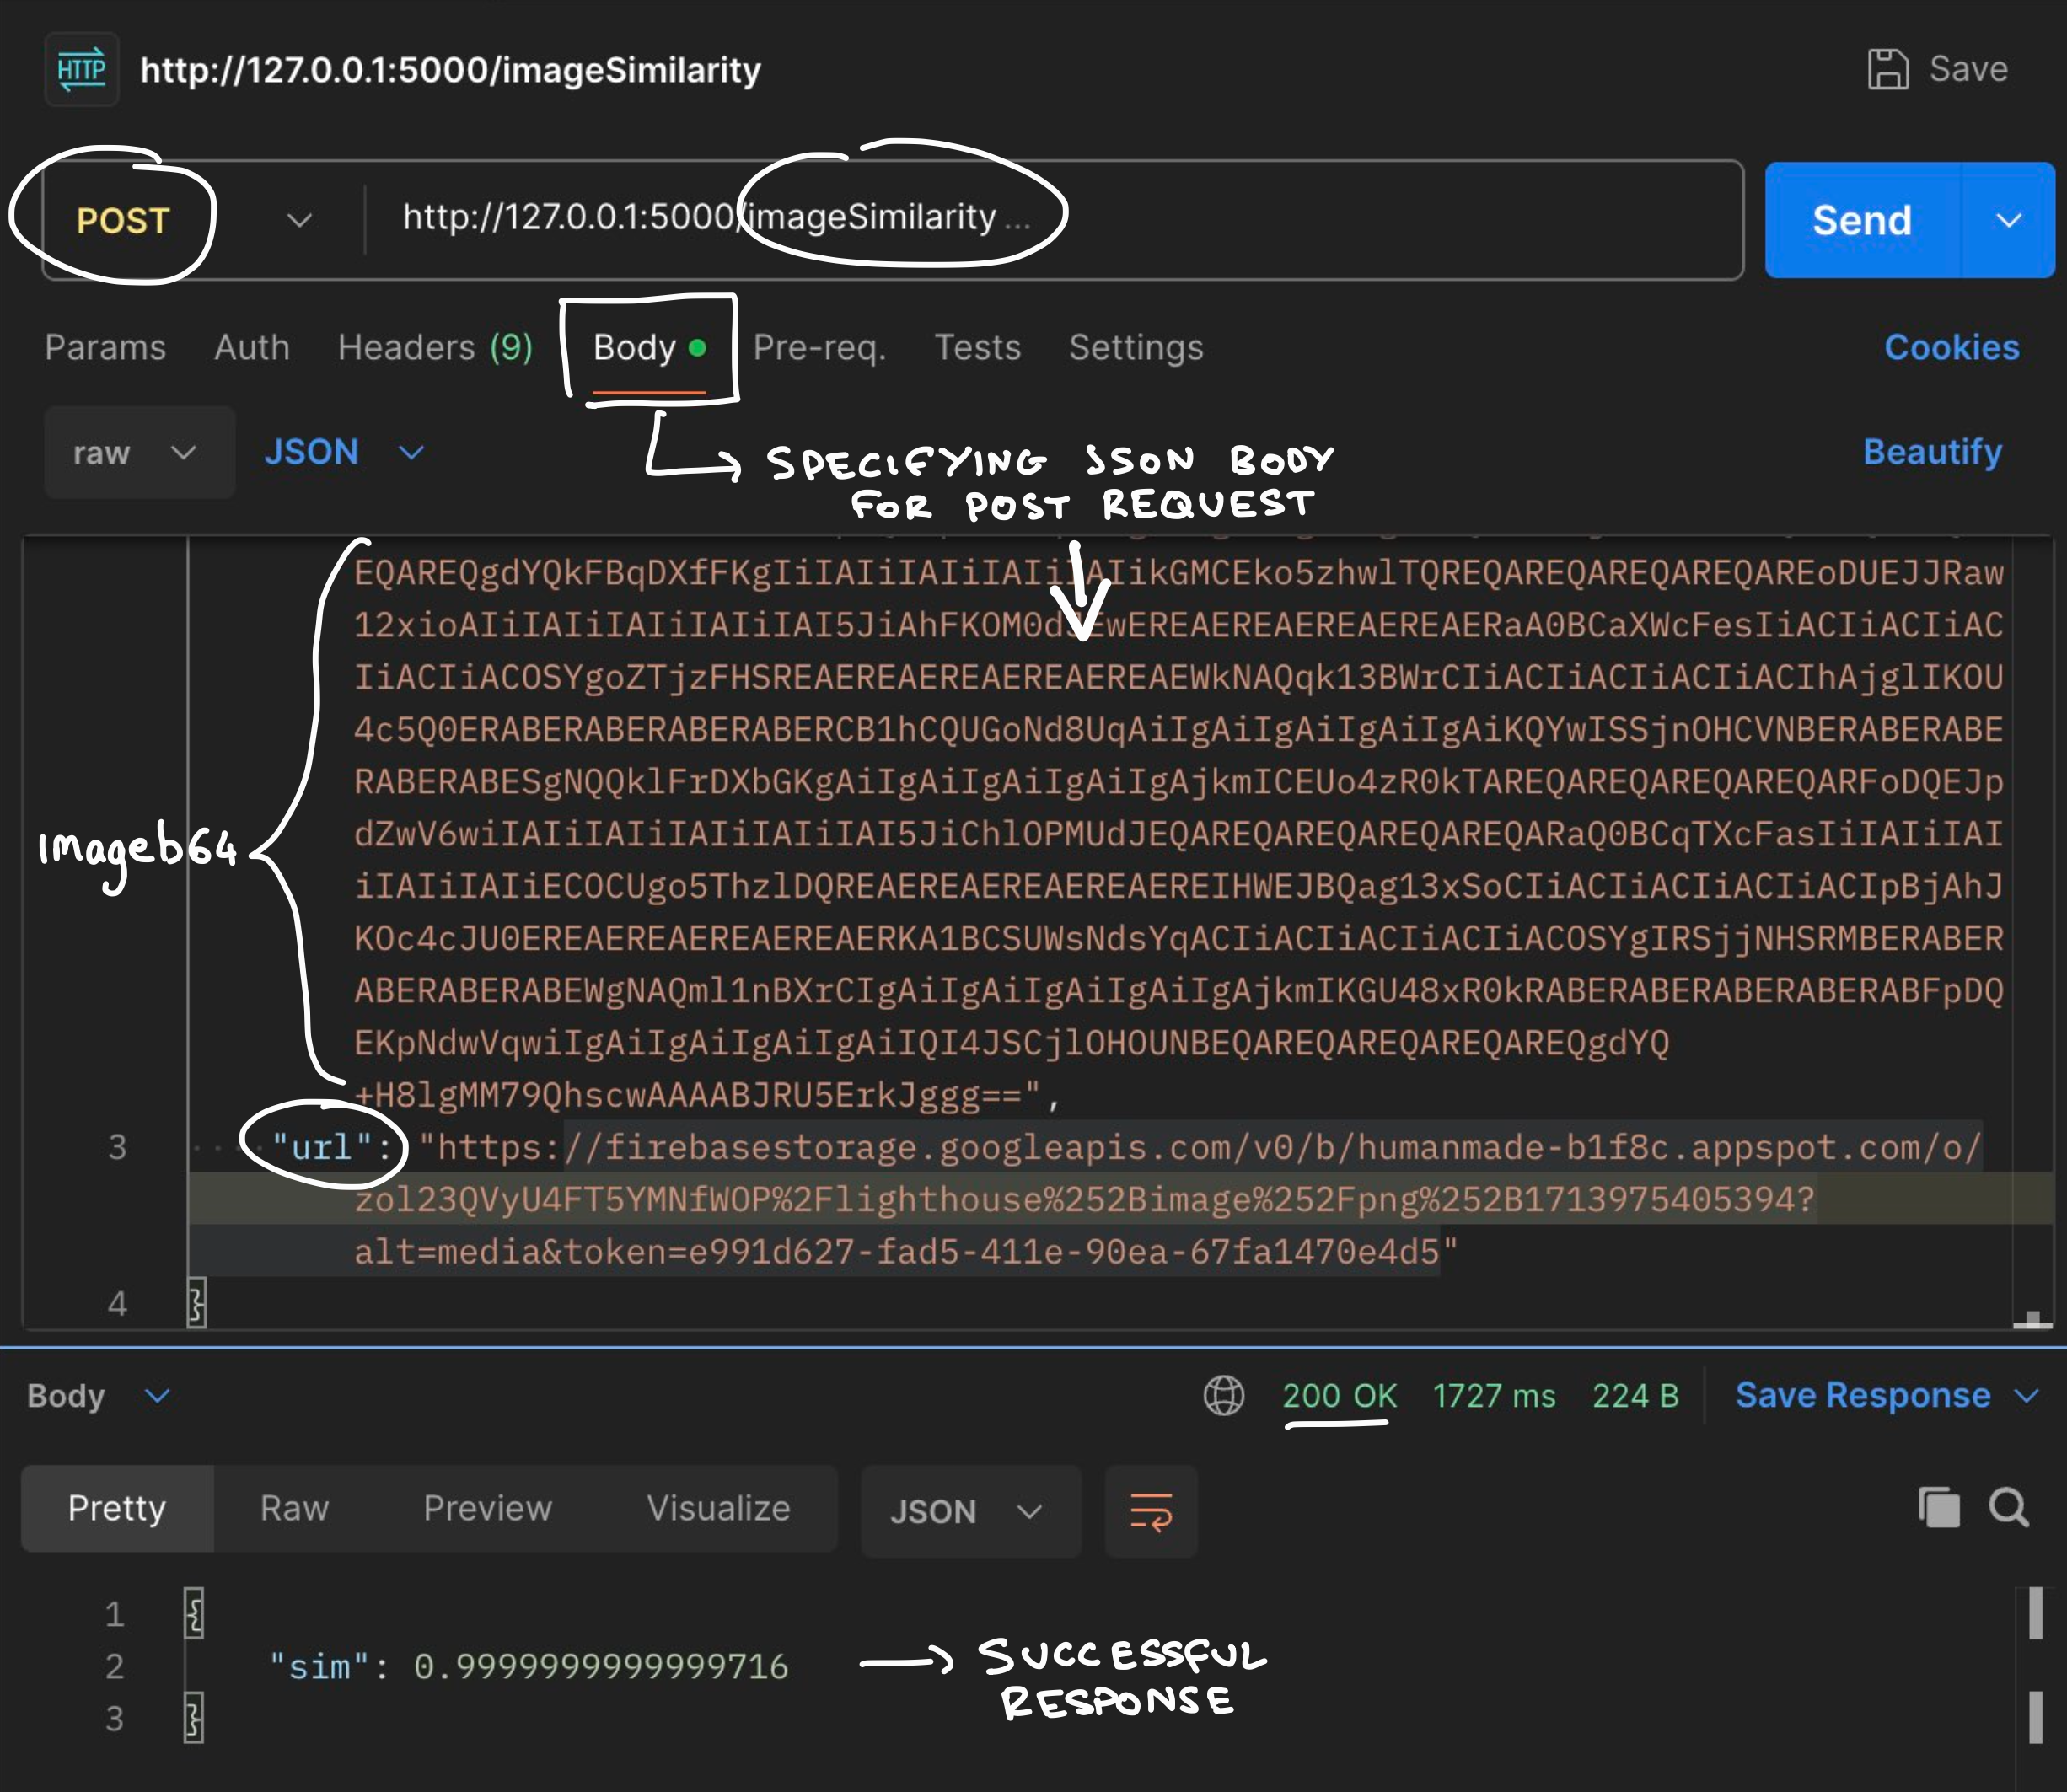
\includegraphics[scale=0.4]{postman2.png}
    \caption{The full process of performing a transaction end-to-end}
\end{figure}
\noindent Here, we test the \verb|/imageSimilarity| API endpoint belonging to our ML Flask microservice. This involves sending a POST request containing a JSON body of the two images to compare (one in base 64, one as a url). We can see how Postman lets us view and edit everything going into the request, and allows us to alter the body or headers easily. The response returns with status 200 and correctly contains the similarity score `sim' sent back in JSON. (The two images tested here were very similar hence the high score).
\subsection{Lighthouse}
Lighthouse is an open-source automated tool on Chrome for improving the performance, quality and correctness of web apps. Lighthouse provides 4 metrics, and details ways that each can be improved if possible:
\begin{enumerate}
    \item Performance (page load times, time to interactive, etc.)
    \item Accessibility (color schemes, meta tags, etc.)
    \item Best Practices (title tags, etc.)
    \item Search Engine Optimization
\end{enumerate}
Issues were highlighted in the performance and accessibility areas of lighthouse initially, however these were minor and fixed quickly. Accessibility wise, issues involved forgetting meta tags, title tags, and color scheme warnings. Performance wise, there was an issue with the size of the CSS being shipped by Font Awesome, which we use for icons, to the client. This was easily fixed by ensuring we used the minified CSS file containing the icons. Tailwind also uses PurgeCSS to ensure only utility classes being used in the web app are shipped to the client - we can specify a \verb|content| field in the tailwing configuration file, which is the path Tailwind will scan for classes being used.
\begin{lstlisting}
content: ['./src/**/*.{html,js,svelte,ts}'],
\end{lstlisting}
We ended up with near perfect scores for each page:
\begin{figure}[H]
    \centering
    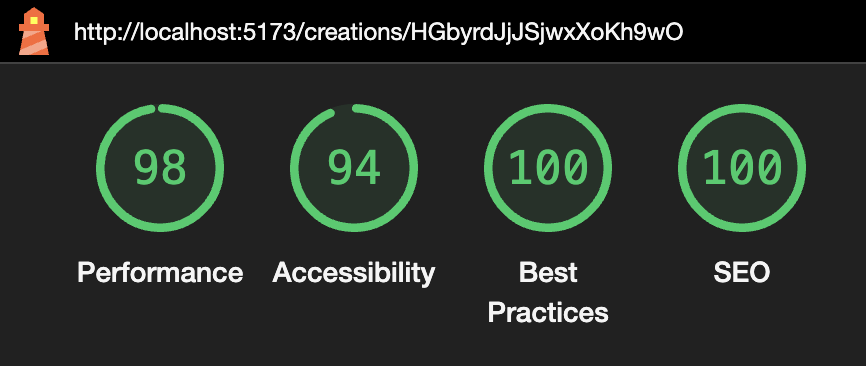
\includegraphics[scale=0.4]{l1.png}
\end{figure}
\begin{figure}[H]
    \centering
    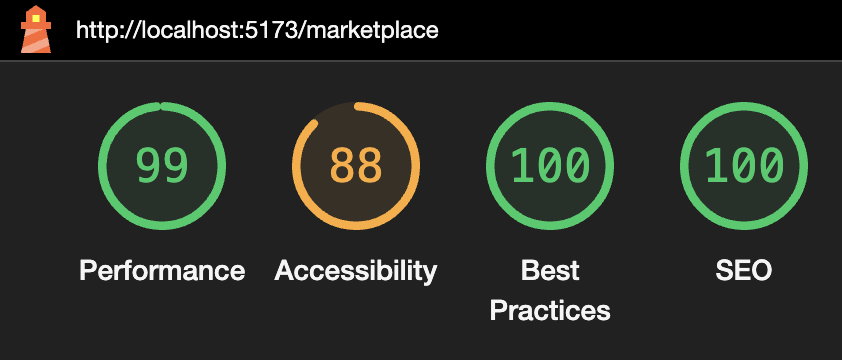
\includegraphics[scale=0.4]{l2.png}
\end{figure}\begin{figure}[H]
    \centering
    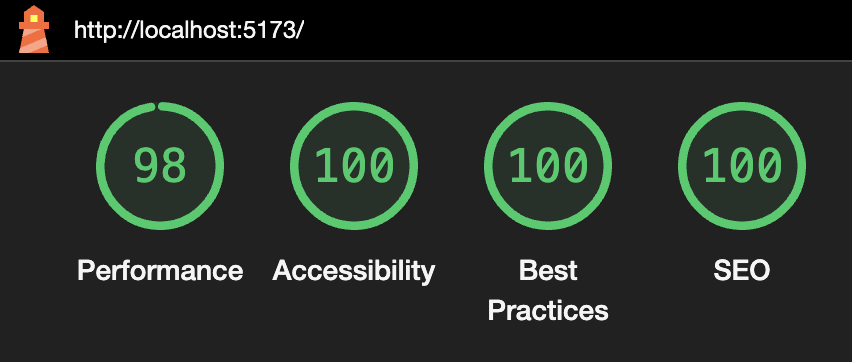
\includegraphics[scale=0.4]{l3.png}
\end{figure}\begin{figure}[H]
    \centering
    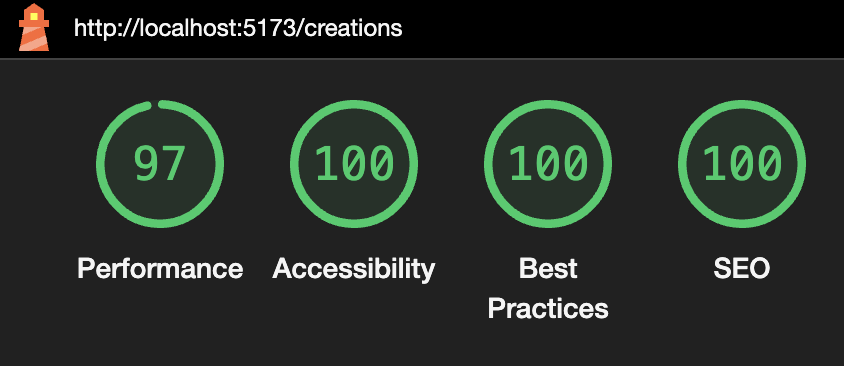
\includegraphics[scale=0.4]{l4.png}
\end{figure}

\noindent Here we see the immediate benefits that using SvelteKit has on SEO and best practices. The performance indicator showed that we have load times below 1 second for each page, as we specified in our nonfunctional objectives.
\subsection{Etherscan}
To test that our blockchain transactions actually worked, we can use Etherscan, which allows us to explore the Ethernet blockchain, as well as related testnets like Sepolia. We can search the chain by address, block, or transaction hash. Pasting the transaction hash 
\begin{lstlisting}
const txHash = await web3.eth.sendTransaction(txObject);
\end{lstlisting}
returned by the \verb|sendTransaction| method into the Sepolia testnet explorer, we can view the date, time and gas prices of the transaction, ensuring they line up with what we know to be true. Crucially, we can also view the input data, which should contain a list of hashes of each file together with the user ID. Indeed, as we hoped, our transactions can be seen on the Sepolia testnet! Below is an example of one:
\begin{figure}[H]
    \centering
    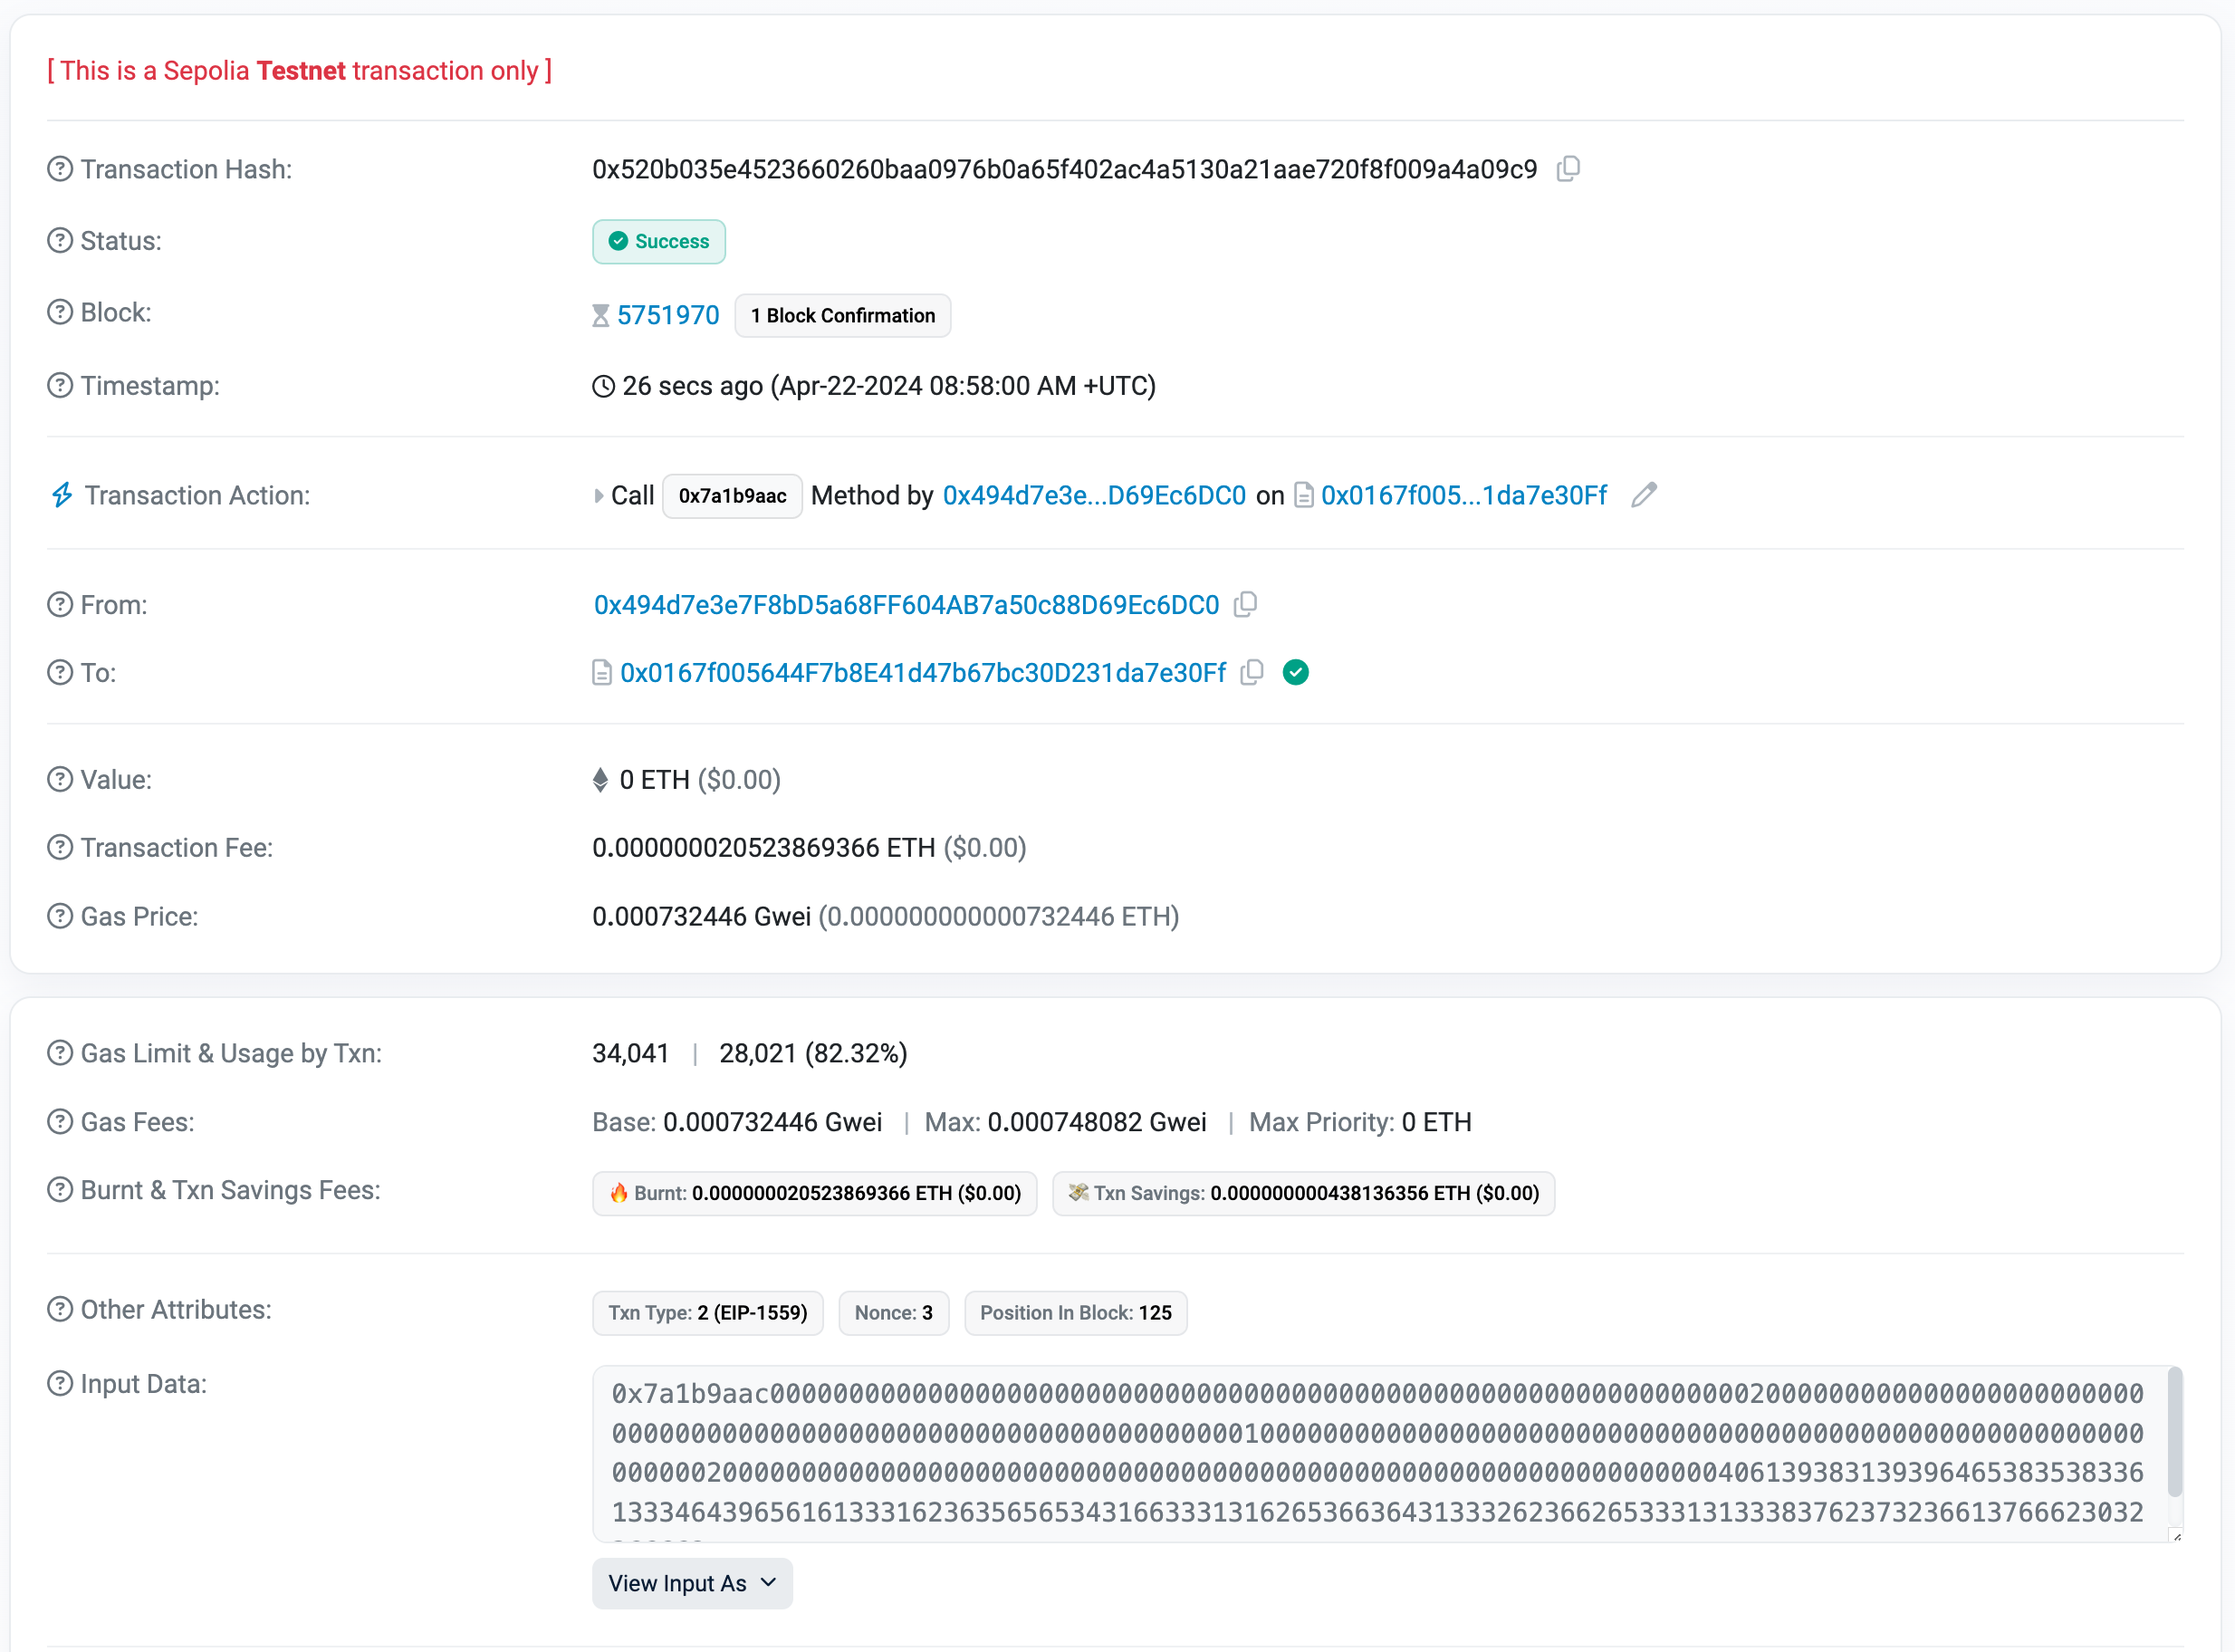
\includegraphics[scale=0.4]{sepolia.png}
\end{figure}

\section{Conclusions}
\subsection{Limitations}
Limitations of the project are mainly due to restrictions on time. Much of the choice of what to work on was dictated by how obvious and easy the work would be. Functionality which was non-trivial and added to the proof-of-concept for HumanMade was prioritised, and areas which could obviously be fleshed out with little need for creativity were understated.
\begin{enumerate}
    \item The marketplace has limited functionality. It is hard to find creations a user may be personally interested in, there is no fuzzy search, a lack of creator profiles and a following system, and no in-built buy or sell functionality. This would take time but be fairly simple to implement with modern technologies and libraries, and would flesh the project out to a fully usable one-stop platform for human creativity.
    \item Currently, we only transact on a blockchain test-net instead of an actual production chain. Test-nets still implement the same cryptographic techniques that make blockchain a secure technology, providing a tamper-proof ledger with which we can record commits on. However, network security may not be as robust; the security of a chain is dependent on the number of nodes participating in the network, and there are fewer of these on test-nets due to their being less financial incentive (the tokens on these test-nets have no real world value). Further, support for a test-net like Sepolia could very well be discontinued.
    
    We did successfully implement a version of the blockchain interface which commits directly to the Ethereum Blockchain with minimal effort, since the transaction process for Sepolia is much the same, however this brings about separate limitations in the form of the high gas fees required for a transaction that (especially at busy times) can be non-negligible.
    \item Creative endeavours are rarely so linear in their progression. Perhaps adding support to branch/merge as in git would help creators express their progression more seamlessly to consumers.
    \item There was a lack of market research undertaken to gauge what features real-life creatives would value. This was due to a lack of interaction and tight deadlines.
    \item Although each commit can be made traceable to a specific user ID, we technically do not know whether that user ID corresponds to a real human. A trivial, extremely useful, yet cumbersome addition would be to add a vetting process ensuring that every user which signs up is a unique human. 
\end{enumerate}
\subsection{Future Development}
As aforementioned, a lot of future development consists of fleshing out obvious areas of the application which were neglected due to tight deadlines.
\begin{enumerate}
    \item To ensure each user ID corresponds to a unique human, we could integrate the platform with a plethora of third party APIs which provide this service, or simply add a Captcha to the Homepage.
    \item There could be an automatic process to check whether a commit which has been transacted on the blockchain has been tampered with. We could create a method which queries Etherscan (they provide their own API service), and checks that the current hashes of the commit line up with the ones stored on the chain.
    \item Additional ML techniques for the automatic verification of auditory and written media (the two other types of creation supported other than visual) could be added. Also, further research could uncover better techniques to gauge the credibility of a human progression across the timeline.
    \item The homepage could be extended to include account customization and creator profiles.
    \item We could transact on a blockchain main-net with no gas prices - blockchains such as Nano \cite{nano} exist but were only discovered after completion of the project, and have much poorer developer ecosystems and so could take more time to integrate with.
    \item The command line utility can be fleshed out further into a full git-like tool, providing branching, merging, deletion and restructuring capabilities of the timeline.
    \item The command line utility could be more accessible to download. Currently a user has to download the files from a GitHub repository, and run \verb|npm install| to install the necessary dependencies. Preferably it would not require technical skill to acquire the utility, and we could instead integrate it with a package manager like Homebrew or Choco.
    \item Adding recommendations (could involve using collaborative filtering ML methods), further filtering options, fuzzy search and creator profiles to the marketplace would help artists find their audience more easily, and help consumers find the art they want to support.  
    \item The concept of a upvote/downvote system was floated early in the project - where creations with more upvotes (potentially a sign of legitimacy) are promoted and shown to more users. Community driven recommendations have been shown to work well across a multitude of social media platforms already.
\end{enumerate}
\subsection{Contributions}
\begin{enumerate}
    \item This is the first platform of its kind promoting specifically human creativity. Whether the platform itself gains popularity or not, it is undeniably a useful blueprint and inspiring proof-of-concept for what will inevitably become a highly in-demand service in some form.
    \item We address some large issues with popular AI detection tools, bringing a holistic viewpoint to the conversation of generative AI detection. It is important to avoid the speciesist trap that generative AI will always be detectable against human creations, as pointed out in the Motivators chapter.
    \item We use an innovative combination of approaches and choices driven by research of the current state of the art and future projections of the technology. This includes tamper-proofing and tracing with blockchain, and progression detection with Convolutional Neural Networks.
    \item The platform also serves as a way for creatives to track their progress on projects, which can be helpful in and of itself, and additionally this can serve as creative inspiration to consumers which can now see the full progression of a creation from beginning to end.
\end{enumerate}
\section{Project Management}
\subsection{Development Methodology}
HumanMade involves a lot of integration and experimenting with cutting-edge technologies that I didn't necessarily have previous experience with, so it was important to keep the development process flexible as well as consistent.

Agile lent much needed adaptability and flexibility to the process. Changes in scope were inevitable due to a foray into a completely new type of platform, incorporating modern technologies - it was much harder than usual to estimate the time it would take to implement say, MetaMask integration or deployment of a smart contract. We worked on the basis of weekly sprints, defined with help from a GANTT chart (specified in the specification document and below) which provided us with a high level timeline and milestones to hit for the project.

\begin{figure}[H]
    \centering
    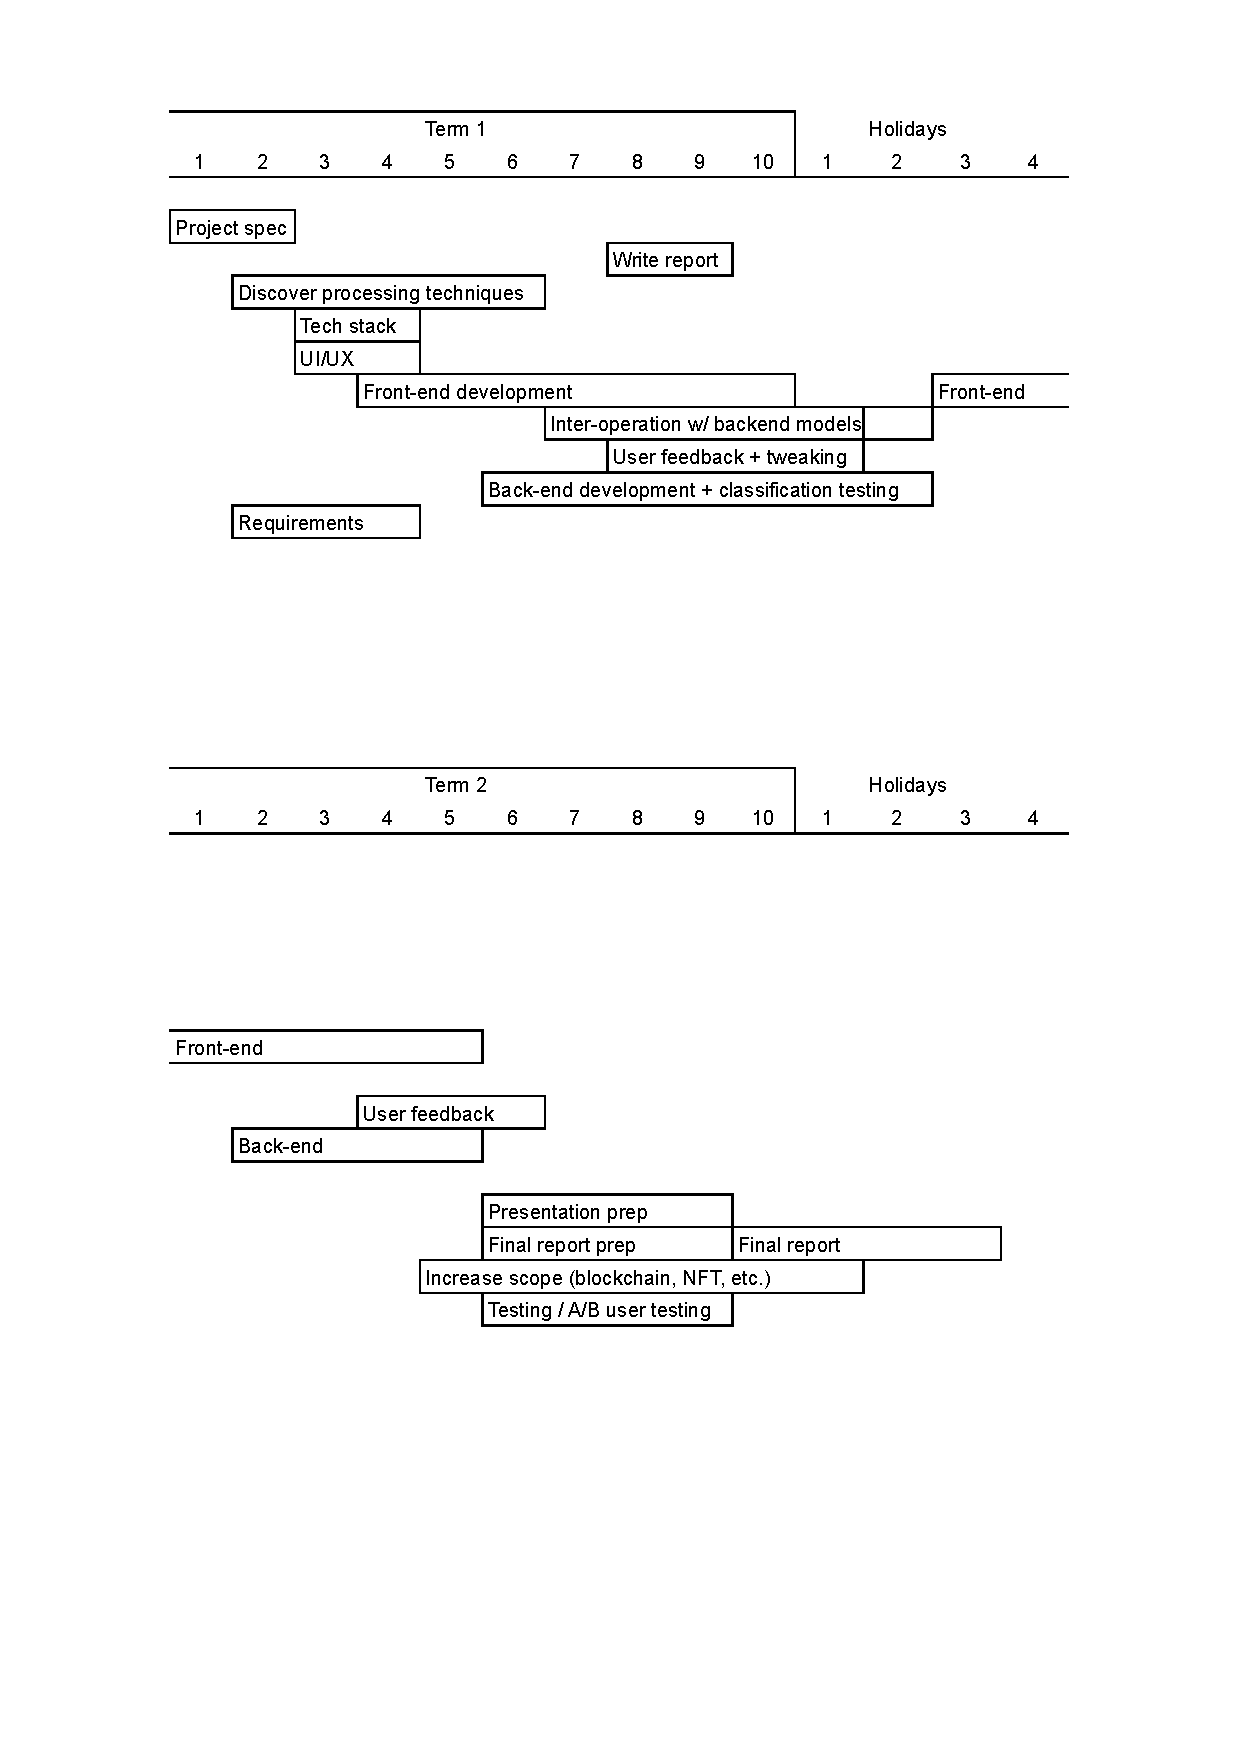
\includegraphics[scale=0.5]{gantt.pdf}
    \caption{The GANTT chart used throughout the project}
\end{figure}
For a sprint, we would set a specific objective to complete a certain component or piece of functionality by the end of the week. Then, we could reassess the GANTT chart and formulate the next sprint, ensuring we stayed on track to deliver a finished product by the end. Agile further helped in this regard by ensuring we broke up work into manageable packages, which could be continuously delivered and integrated into the project. This avoided scenarios where a certain component could be worked on for a substantial period of the project only to not work or integrate correctly. For example, when developing the ML microservice, sprint one was:
\\\\
\textbf{1:} Set up a basic \verb|/imageSimilarity| POST endpoint with Flask:
\begin{enumerate}
    \item Create a new Python environment, installing the relevant libraries required with \verb|pip| (Flask, base64, jsonify).
    \item Write Flask boilerplate code.
    \item Write an \verb|@app.route| endpoint of type POST, which takes the JSON body of the post request and expects a \verb|url| and \verb|imageb64| property.
    \item Implement a primitive image similarity function with the ssim.js library.
    \item Return the similarity score and status code 200.
    \item Test the endpoint works using Postman.
\end{enumerate}
While sprint two then delved deeper, expanding on the image similarity computation.
\\\\
\textbf{2:} Create an improved image similarity method:
\begin{enumerate}
    \item Look into available TensorFlow Deep learning networks for images.
    \item Write and research the needed utility functions and pipeline for image pre-processing.
    \item Figure out how we can extract a high-level feature vector of each image using such a network (classification or otherwise).
    \item Compare the two feature vectors with some measure, most likely cosine similarity.
    \item Replace the current image similarity function in the Flask endpoint, and test the correctness of the code using Postman and images of differing similarity.
\end{enumerate}
\subsection{Tools}
To aid with the above methodology:
\begin{itemize}
    \item Trello was used for bug tracking and defining sprints and tasks to complete
    \item GitHub was used for version control, allowing development of experimental features on separate branches, and providing an up-to-date backup for work by making it easy to consistently commit progress.
    \item Visual Studio Code was used for development. This integrated environment has syntax and completion support for many of the technologies that were being used including Svelte, Python, and TypeScript. Further, all reports were written with the Latex extension in VSCode, which provides an accurate word count and instant recompilation of the PDF upon saving any changes, improving efficiency and focus on the writing.
    \item Goodnotes is an application on the iPad which allows a user to take handwritten notes or notate diagrams. This was used for some figures throughout the final report, and to sketch and note ideas early on in the project.
\end{itemize}
\subsection{Ethics, Social Issues \& Law}
\subsubsection{Data Collection \& Transfer}
Beyond an email address to sign up to the platform, no personal data is collected. Users have the choice on what to upload to their progress timelines, and can share as much or as little of the creative process as they would like, although there is an incentive to be as transparent and thorough as possible with the documentation of the creation. Either way, we must ensure that we adhere to GDPR data protection guidelines for the EU market. We make sure to adhere to each of the four GDPR guidelines closely:
\begin{enumerate}
    \item Transparency. We ensure that we are transparent in the way in which we transfer data across microservices and where data is stored by adding a disclaimer at the bottom of the Homepage:
    \begin{lstlisting}
        <p>Files uploaded to progress timelines will be processed by a microservice running on Google Cloud. All data is stored using Firebase.</p>
    \end{lstlisting}
    \item Purpose Limitation. We do not use data for purposes other than what is required for the functionality of the web app.
    \item Data Transfer Encryption. We host our microservice and web app on Google Cloud, which provides encryption in the form of HTTPS. No private keys are transferred across networks, as mentioned in the Blockchain Interface implementation section.
    \item Data Rights. We ensure the user has the ability to delete any commit they have added to any progress timeline. Data is fully deleted from the database and is not stored anywhere else.
\end{enumerate}

\subsubsection{Artistic Value}
It is probable that AI will likely get so good that any techniques used to suss generation at all will eventually be futile (AI could probably generate a realistic-looking progress timeline at some point with ease if required), hence why we stressed on building a holistic platform which can at least deter purely AI generated creation. But eventually deeper questions must be posed in relation to the existence of such a platform - what actually makes our creativity more valuable than an AIs? And to answer that, we might ask, what does it mean to be creative or to possess the ability to experience reality in the first place? Is conciousness a physical property of all matter (panpsychism), or is there something special about the specific mechanisms in our brains (quantum conciousness), and so should they be treated differently from any technological artefact? At what point (assuming even just a steady rate of progress), if ever, should we accept and celebrate fully AI generated creations? All of these questions are exceedingly difficult to answer, if they have answers at all, but they spawn social considerations which should be made in the event such a platform gains mass popularity. Such platforms could perpetuate an arguable negative (depending on the answers to those questions) shift in artistic value, toward prioritising authenticity rather than intrinsic artistic qualities.
\subsection{Project Evolution}
The initial ideas for the project were about fleshing out a fully functional web platform for human creation, perhaps with features like creator profiles, followers, a full marketplace and other areas of web app development that could have been expanded on, some mentioned in Future Development. However, soon after market research and analysis, and considering future projections of the technology, the focus of the project shifted to building multiple smaller components. The aim was that these components formed more of a proof-of-concept, an ecosystem of tools and features that all contributed towards making it as seamless as possible for human creativity to take place on the platform, and as inconvenient as possible for purely AI generated creations to be promoted. In the end we think this change in direction paid off.
\\\\
The project also evolved once more, with a larger chunk of time being spent on implementing a seamless blockchain interface for commits. Given the enjoyable, fascinating and cutting-edge nature of the implementation, this change in priorities was not disappointing, and in fact was legitimized upon further thought. As aforementioned in the Final Design chapter, we may soon live in a world where human art is more rare and highly coveted, and it may therefore be vital that a creation and important milestone commits associated with it are traceable back to the original human creator, and cannot be tampered with by any third party, including the owner of HumanMade. This is of course speculation, but is heavily implied by the initial research that took place for the project.
\subsection{Progress against Original Objectives}
\begin{figure}[H]
    \centering
    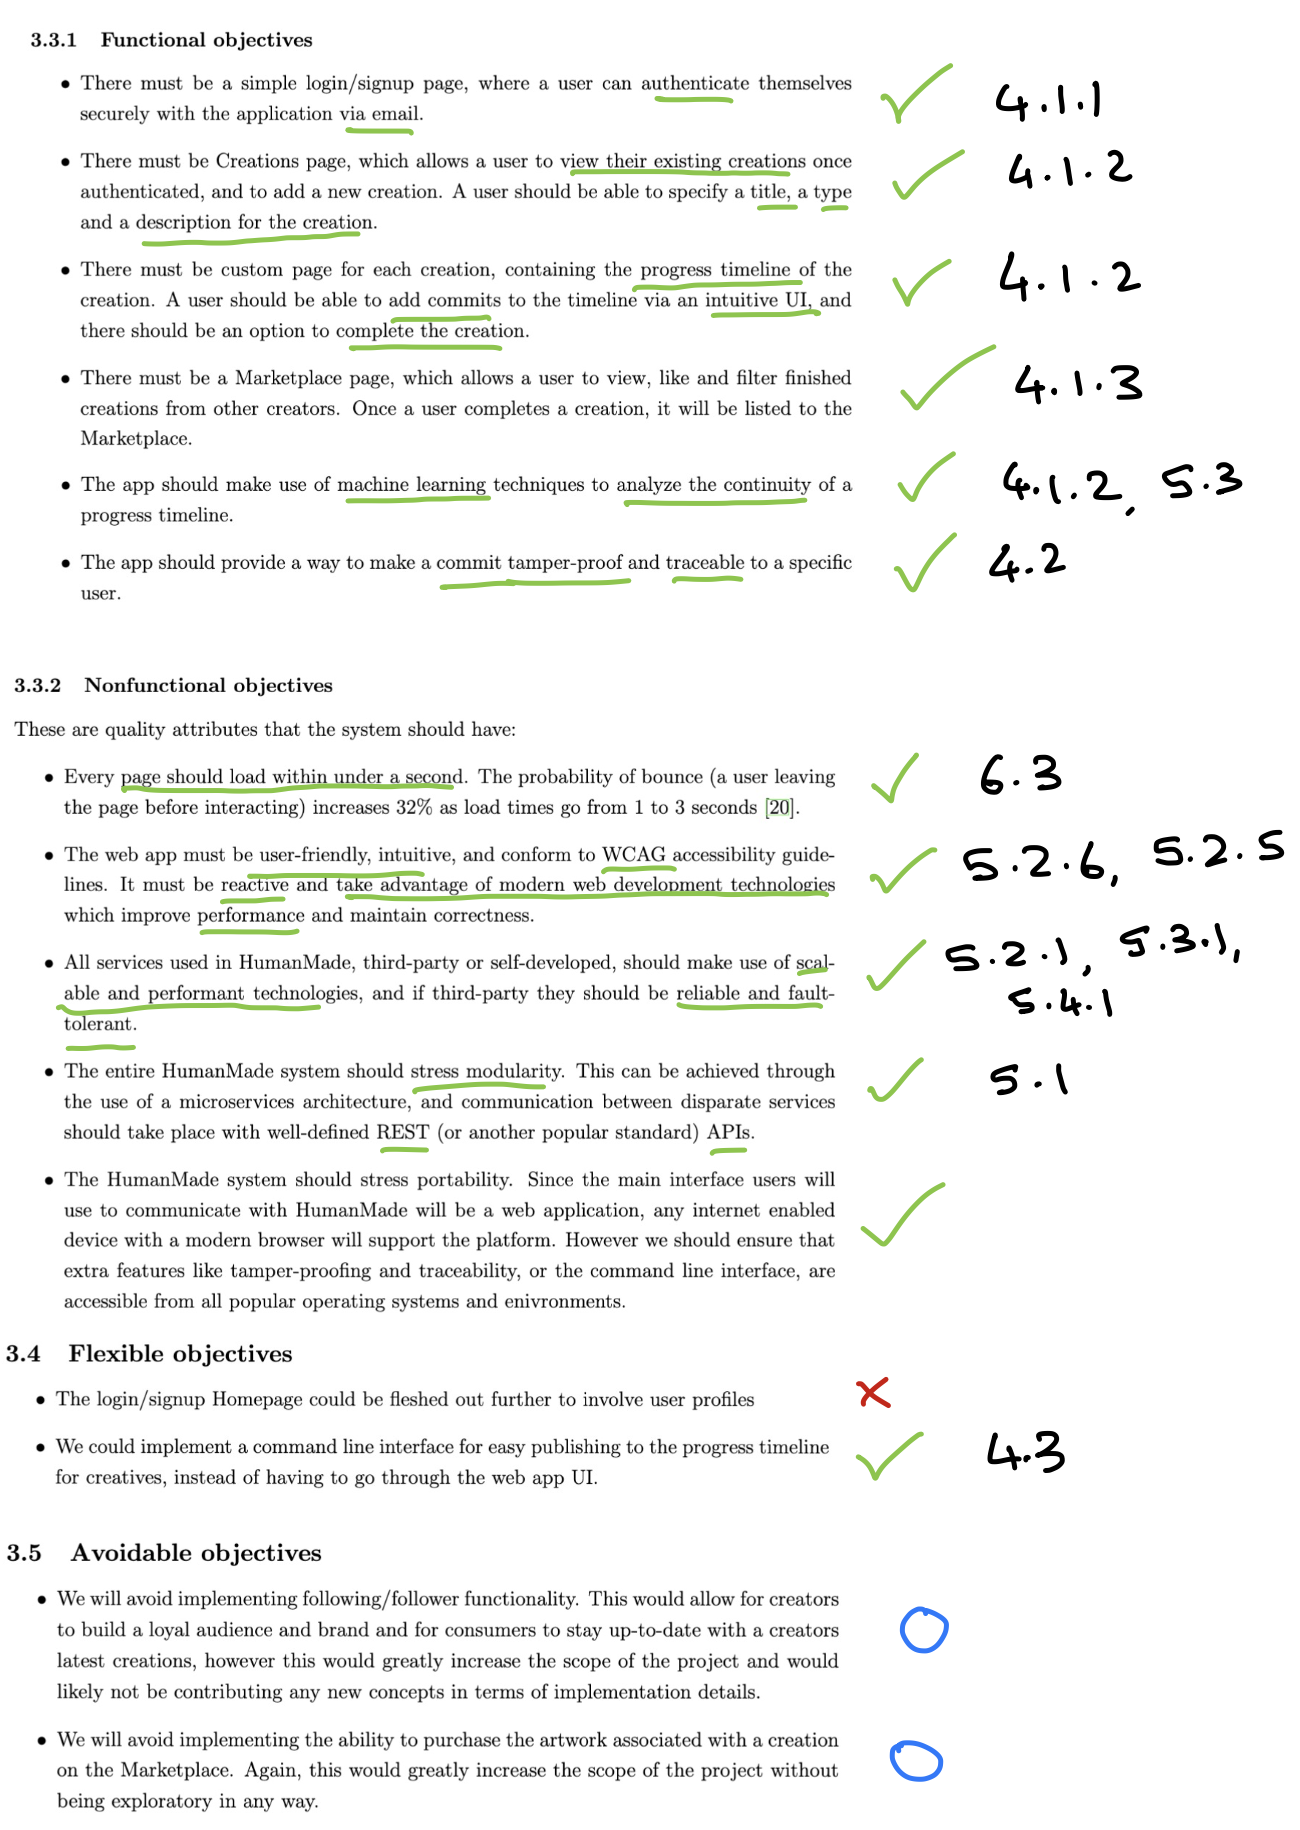
\includegraphics[scale=0.7]{objectives.png}
\end{figure}
As shown on the above figure, progress against original objectives was almost flawless. Noted next to each objective are the sections in which we achieved them. We only failed to achieve one flexible objective, which involved fleshing out a user profile system.

\newpage
\bibliography{finalReport}

\end{document}